\documentclass[a4paper,11pt,twoside]{report}

\hyphenation{PrologPF}

\newcommand{\todo}[1]{\vbox{
                            \hrule 
                            \hbox{\strut \vrule{} {\textbf{todo:} #1} \vrule}
                            \hrule 
                           }}


%\renewcommand{\topfraction}{.8}
%\renewcommand{\bottomfraction}{.8}
%\renewcommand{\textfraction}{.2}
%\renewcommand{\floatpagefraction}{.8}
%\renewcommand{\baselinestretch}{1.1}
\setlength{\parindent}{0pt}
%\setlength{\parskip}{3pt}

% This is to change the width of a page
%\textwidth 15.3cm


\def\postscript{{\sc postscript}}
\input{psfig}

\psfull

\usepackage{rotating}
\usepackage{subfigure}
\usepackage{latexsym}
\usepackage{alltt}

%%%%%%%%%%%%%%%%%%%%%%%%%%%%%%%%%%%%

\includeonly{title/title,
              intro/intro,
              background/background,
              bfp_depth/bfp_depth,
              cut/cut,
              functions/functions,
              case/case,
              kappa/kappa,
              sok/sok,
              conclusions/conclusions,
              system/system,
              benchmarks/benchmarks,
              kappa_macro/kappa_macro,
              references/references
	}

%%%%%%%%%%%%%%%%%%%%%%%%%%%%%%%%%%%%

\begin{document}

\bibliographystyle{ijl20}

\setlength{\parskip}{8pt}

\pagestyle{empty}

% The cover page 

{  \begin{center}
\vspace*{\fill}
\LARGE\bf 
PrologPF: Parallel Functional Logic\\ on the Delphi Machine \\
\vfill
\vfill
\vfill
\Large
 \bf Ian Lewis\\[6mm]
Girton College\\
University of Cambridge\\
\vfill
\centerline{\psfig{figure=title/ps/culogo.ps}}
\vfill
\large \bf
A dissertation submitted for the degree of\\
Doctor of Philosophy\\[4mm]
April 1998\footnote{This version created \today.}\\
\vspace*{\fill}
\end{center}
}

\newpage
%\vspace*{\fill}
{\bf \Huge Abstract}

\vspace{12pt}
PrologPF is a parallelising compiler targetting a distributed system of general purpose
workstations connected by a relatively low performance network.  The source language
extends standard Prolog with the integration of higher-order functions.

The execution of a compiled PrologPF program proceeds in a similar manner to
standard Prolog, but uses \textit{oracles} in one of two modes.  An oracle
represents the sequence of clauses used to reach a given point in the problem
search tree, and the same PrologPF binary can be used to \textit{build} oracles,
or \textit{follow} oracles previously generated.

The parallelisation strategy used by PrologPF proceeds in two phases.  An
initial phase searches the problem tree to a limited depth, recording the oracles
representing the discovered incomplete paths.  
In the second phase these oracles are allocated, with
the complete program, to the available processors in the network.  Each processor
follows its assigned oracles and fully searches the subtree referenced by each
oracle, sending solutions back to a control processor.  Processor failure can
be accomodated by the reassignment of the affected oracles.

For a problem requiring \textit{all} solutions to be found, execution completes
when all the distributed processors have completed the search of their assigned
subtrees.  If \textit{one} solution is required, the execution of all the path
processors is terminated when the control processor receives the first
solution.

The presence of the metalogical Prolog predicate \textit{cut} in the user
program conflicts with the use of oracles to represent valid open subtrees.
PrologPF promotes the use of higher-order functional programming as an
alternative to the use of \textit{cut}.  The combined language shows that
functional support can be added as a consistent extension to standard Prolog.




% Ack. page 

\parskip 10pt
\newpage
\pagestyle{plain}
\pagenumbering{roman}
%\vspace*{\fill}
\vfill 
\vfill
{\bf \Huge Acknowledgements}

\vspace{15pt}
I would like to thank my wife, daughter, cat dog etc.





% Declaration, Publication and trademark.

\newpage
{\bf \Huge Declaration}

\vspace{10pt}
Except where otherwise stated in the text, this dissertation is the result of my own work and is not the outcome of work done in collaboration. This dissertation is not substantially the same as any I have submitted for a degree or diploma or any other qualification at any other University. No part of this dissertation has already been, or is being currently submitted for any such degree, diploma or other qualification.


\vspace{40pt}


{\bf \Huge Trademarks}

\vspace{10pt}
Ethernet is a registered trademark of Xerox Corporation. \\
UNIX is a registered trademark of Novell. \\


\newpage
\setcounter{tocdepth}{2}
\tableofcontents




% List of figures
\newpage
\addcontentsline{toc}{chapter}{List of Figures}
\listoffigures


\vfill
\vfill
\vfill
\vfill

% List of tables
\newpage
\addcontentsline{toc}{chapter}{List of Tables}
\listoftables


\newpage
\pagenumbering{arabic}



\setlength{\parskip}{8pt}

\pagestyle{headings}

\chapter{Introduction}
\label{intro}

PrologPF is named after \textbf{Prolog} in \textbf{P}arallel with
\textbf{F}unctions.

PrologPF is an implementation of a parallel logic language with the
following key features:
\begin{itemize}
\item{The target environment for the compiled binaries is a distributed
  network of heterogeneous processors with comparatively slow communication
  links, such as an ethernet or wide-area internet.}
\item{The failure of individual processors during the parallel computation
  can be accommodated without undue performance penalty}
\item{The language is an extension of sequential Prolog \cite{DEDC96}.}
\item{OR-parallelism is provided through the use \textit{oracles}
  to name branches
  in the search tree to be allocated for distributed search
  (\cite{CA87} and section \ref{delphi_background}).}
\item{PrologPF extends the Prolog base language with
  support for the definition and deterministic
  application of higher-order functions
  in a manner consistent with the parallelisation method.}
\end{itemize}

In comparison with other functional logic languages\footnote{Chapter
\ref{background} provides a detailed comparison with related work.},
PrologPF uses the efficient but incomplete
depth-first search of standard Prolog, and the deterministic eager
evaluation of function terms as in functional languages such as
Standard ML \cite{MTH90}.  Using the comparison drawn by Paulson and
Smith in \cite{PS91},  PrologPF is a programming language for
\textit{realists} rather than 
a theorem proving system for \textit{purists}.

The development of the PrologPF system has provided a vehicle for the
analysis of scheduling algorithms suitable for the discovery and 
distributed allocation of
oracles.
The integration of functions into the
logic language provides a means of avoiding the undesirable
characteristics of some extra-logical Prolog predicates that would conflict with
the parallelisation technique used.

Considerable effort has been made to maintain the
portability of PrologPF.  The compiler
should provide a sound basis for further research such as:
\begin{itemize}
\item{Improvement of the strategies to
  be used for oracle distribution.}
\item{Extension of the oracles into
  the function evaluation trees.}
\end{itemize}

A processor designed to execute the compiled PrologPF programs is
called a \textit{path processor}, with the general architecture suitable
for creating and following oracles being called the \textit{Delphi
Machine}.  The previous implementation of the Delphi Machine by Klein
\cite{Kle91},
further investigated by Saraswat \cite{Sar95}, is called in this dissertation
\textit{DelphiKS}.

\subsection{Prolog}
%%%%%%%%%%%%

The definition of Standard Prolog is contained in \cite{DEDC96}, and many
examples of practical use of the language in \cite{CM87}.

Prolog is a logic language based upon the first-order predicate calculus.  A good
introduction to the predicate calculus is provided by Lloyd in \cite{Llo84}.
A Prolog program
is a list of \textit{definite Horn clauses}, i.e. clauses containing exactly one
positive literal, these programs called \textit{definite programs} by Lloyd in
\cite{Llo84}.  A clause with no positive literals defines the \textit{query}.
Each clause is a conjunction of literals.  A \textit{literal} is a predicate with
a list of terms as arguments.  A \textit{term} can be a \textit{constant} (i.e.
a string or number), a \textit{variable}, or a compound term. 
Variables are string constants beginning with a capital letter or \texttt{\_{}}.
A \textit{compound term}
is a string constant with a list of terms as arguments.

A clause containing one literal (which is positive) is called a \textit{fact}.  Clauses
with more than one literal (of which one is positive) are called \textit{rules}.

Prolog syntax requires that the positive literal appears at the head of the clause,
while the negative literals (called the \textit{body})
follow after the symbol ``\texttt{:-}''.  The conjunction of
the negative literals is represented by ``\texttt{,}''.
Clauses end with a full-stop ``.''.

Comments are surrounded by \texttt{/*\ldots*/} or by \texttt{\%\ldots<newline>}.

Examples of Prolog facts are:
\begin{verbatim}
a.              % the proposition a
a(b).           % relation a holds for term b
b(c).           % relation b holds for term c
a(b,c).         % relation a holds with arguments (b,c)
a(X).           % relation a holds for any argument term X
\end{verbatim}

Examples of Prolog rules are:
\begin{verbatim}
a :- b.         % asserts a & not(b), i.e. a <= b
a :- b,c.       % a & not(b) & not(c), i.e. a <= b & c
a(X) :- b(X).   % relation a holds for term X if
                     relation b holds for the same term
\end{verbatim}

\textit{Unification} is the process of matching each argument of a subgoal with
those in the head of a candidate clause.  Genesereth and Nilsson describe the
process and provide a pseudo-code algorithm for unification in \cite{GN86} pages 66-69.
The process arrives at a \textit{most general unifier} when the unification is successful
and leads to \textit{failure} and subsequent backtracking if unsuccessful.  The
unifier represents a set of variable bindings which would make the subgoal and the
head of the candidate clause identical.  These bindings form a context within which the
proof process continues.

In solving a query such as \texttt{:- a(X,Y),b(Y)} a sequential Prolog interpreter
will proceed from left-to-right, finding a solution for each subgoal in turn.  To
find a solution for a given subgoal (i.e. \texttt{a(X,Y)} first), the interpreter will
try the program clauses in a top-down order.  After a successful unification with the
head of a rule, the interpreter will attempt to solve left-to-right
the new goal defined by the
instantiated body of that rule.  On failure of this new subgoal, the top-down
search through the program clauses will continue.

\subsection{Parallelism}
%%%%%%%%%%%%

Logic languages have potential for faster execution through the
exploitation of the available parallelism \cite{Tic91}.  The 
declarative code can be parallelised in several ways, illustrated by the
following program fragment:

\begin{tabular}{l l l}
$a(X)$   &$\Leftarrow$ &$b(X,Y)\  \&\  b(Y,Y)$\\
$b(1,2)$ &             &\\
$b(2,2)$ &             &\\
\end{tabular}

A query can be expressed such as $a(Z)$
with the intended meaning that the system should
step through the program facts and rules to arrive at values for $Z$
for which $a(Z)$ is provable.

The opportunities for parallel execution
within the proof search process include:
\begin{description}
\item[AND-parallelism]{The subgoals $b(X,Y)$ and $b(Y,Y)$
  in the body of the rule for $a$ may be searched in
  parallel to arrive at common solutions for $Y.$}
\item[OR-parallelism]{The multiple rules for $b$ can be searched in
  parallel to find solutions for $b(X,Y)$ or $b(Y,Y)$.}
\item[Unification parallelism]{The subgoal $b(X,Y)$ can be solved if
  suitable values are found for both $X$ and $Y.$  In the selection of
  a candidate rule, these arguments can be unified in parallel with the
  formal arguments in the selected rule (e.g. ($1,2$)).}
\end{description}

PrologPF implements OR-parallelism through the use of \textit{oracles}
on an extended abstract machine called the \textit{Delphi machine}.
Further introduction is given in section \ref{delphi_background}, a
review of previous work on the Delphi machine in Chapter \ref{background},
and a detailed analysis of the technique in Chapter \ref{bfp_depth}.

\subsection{Functions}
%%%%%%%%%%%%

This section provides some background and an introduction to the use
of functions in PrologPF.
A detailed analysis of the functional support provided in PrologPF is
given in Chapter \ref{functions}.

Functional \textit{reduction} refers to the transformation of a reducible
term to a normal form which is
considered to be irreducible.  When this process is
embedded in the code produced by compilation of a functional program, the
reduction is called \textit{evaluation}.

The execution of Prolog programs is limited to top-down, left-to-right
search with candidate clause matching through unification.  The
terms given as actual arguments to relations as subgoals are unified 
directly with the corresponding terms given as formal arguments in the
head of the candidate program clause.  Thus the Prolog system provides no
direct
support for the \textit{evaluation} of parameters (with the exception
of the \texttt{is} relation and related arithmetic terms, see Chapter \ref{functions}).

However, equivalent relations can be defined representing the required
functions in a \textit{flat} form, with the result given as an
auxiliary argument.  For example the \texttt{length} function to
produce the length of a list can
be defined in Prolog as:\\

\begin{minipage}[h]{\textwidth}
\begin{verbatim}
length([],0).
length([X|Y],N) :- length(Y,N1), N is N1 + 1.
\end{verbatim}
\end{minipage}

The \texttt{length} example illustrates the use of an auxiliary argument to
hold the result, and the flat form imposed by the exclusive use of 
relations, with the exception of the special \texttt{is} which evaluates the
arithmetic expression given as the second argument.  With the definition
given above, the relation \texttt{length} can be used in a subgoal to
produce a variable binding for the length of a given list.  The Prolog
definition should be viewed in the context of these comments from
\textit{Compiling with Continuations}, by Appel \cite{App92}:

\textit{The beauty of FORTRAN -- and the reason it was an improvement over
assembly language -- is that it relieves the programmer of the
obligation to make up names for intermediate results.  For example we write
$x = (a + b) * (c + d)$ instead of the assembly language:\\
\centerline{$r_1 \leftarrow a + b$}\\
\centerline{$r_2 \leftarrow c + d$}\\
\centerline{$x \leftarrow r_1 \times r_2$}\\
}

For comparison with standard Prolog, a definition of \texttt{length}
as a function in PrologPF would be:

\begin{verbatim}
fun length([])    = 0;
    length([X|Y]) = 1 + length(Y).
\end{verbatim}

With the functional definition in PrologPF, the term \texttt{length(X)} can appear
anywhere in an argument term to represent the length of the list argument
\texttt{X}.

The reduction of functional expressions can be defined in terms of the
\textit{lambda calculus}\footnote{An introduction to the lambda calculus can be
found in \cite{HS86}, while Barendregt provides encyclopedic coverage in \cite{Bar84}.}
In lambda notation, terms are limited to:
\begin{description}
\item[Variables.]{Usually denoted by a constant string such as $x$.}
\item[Constants.]{Also denoted by constant strings, leaving context to
  differentiate constants and variables.}
\item[Applications.]{I.e. the application of a function $s$ to an
  argument $t$; both $s$ and $t$ may be arbitrary lambda terms.  An application
  can be represented by the simple juxtaposition of the function and argument,
  e.g. $s\ t$.  Application is generally defined to be left-associative, i.e.
  $s\ t\ u \equiv (s\ t)\ u$.}
\item[Abstractions.]{I.e. function definitions in the lambda notation, the function
  mapping an argument $x$ to a term $t$ being $\lambda x.\ t$.}
\end{description}

The application of an abstraction to an argument term relies upon the
principle of \textit{substitution}.  For example in the term
$(\lambda x.\ t)\ a$ the reduction of the application term proceeds with
the substitution of the argument $a$ for the variable $x$ in the term $t$, the
result denoted $t[a/x]$.  For example, $(\lambda x.\ x\ x)\ a$ reduces to
$(x\ x)[a/x]$, i.e. $(a\ a)$.

The $x$ in the above example is referred to as a \textit{bound} variable, representing
the formal argument of the lambda abstraction with the extent of its scope limited to
the abstraction body.  Terms within nested lambda abstractions may contain variables
other than those of the immediately enveloping lambda-term, and these variables are
said to be \textit{free} within that abstraction.  For example, in
$\lambda x.( \lambda y.\ x\ y)$ the variable $x$ is said to be free in the term
$\lambda y.\ x\ y$.  The set of free variables in a term $s$ can be denoted $FV(s)$, and 
the bound variables $BV(s)$.

Reduction in the lambda calculus is based upon three transformations of lambda terms:
\begin{description}
\item[1. $\alpha$-conversion.]{The constant representing the name of the bound variable
  in a lambda abstraction can be consistently changed throughout that expression, to any
  value that is not a free variable in the expression.  I.e. $\lambda x. s \rightarrow_\alpha
  \lambda y.s[y/x]$ provided $y \not \in FV(s)$}
\item[2. $\beta$-conversion.]{The application of a lambda abstraction to an argument
  term is equivalent to the body of the abstraction with the argument term 
  substituted for the bound variable.  I.e. $(\lambda x.\ s)\ t \rightarrow_\beta
  s[t/x]$.}
\item[3. $\eta$-conversion.]{A lambda abstraction which applies a term to the bound
  variable is equivalent to that term,
  provided the bound variable is free in the term.  I.e. $\lambda x.\ s\ x \rightarrow s$
  provided $x \not \in FV(s)$.}
\end{description}

The evaluation of lambda terms is equivalent to the repeated application of 
$\alpha$-, $\beta$- and $\eta$-conversions until there is nothing more to be 
evaluated.  When no more reductions are possible except for $\alpha$-conversions
the term is said to be in \textit{normal form}, and is \textit{irreducible}.

Within this framework there is still considerable flexibility in the selection of
the conversion to be applied at each step, and the selection of the subexpression
(the \textit{redex}) within the lambda term to be reduced.  For example, given:\\
\centerline{$(\lambda x.\ x\ x)\ ((\lambda y.\ a)\ a)$}\\
then an $\alpha$-conversion could be applied to either of the lambda-abstractions,
resulting in:\\
\centerline{$(\lambda y.\ y\ y)\ ((\lambda z.\ a)\ a)$}\\
or a $\beta$-conversion applied to the second application:\\
\centerline{$(\lambda x.\ x\ x)\ a$}\\
or a $\beta$-conversion applied to the first application:\\
\centerline{$((\lambda y.\ a)\ a)\ ((\lambda y.\ a)\ a))$}

Any implementation of a functional programming language based upon the lambda
calculus defines a \textit{reduction strategy}.  For the purposes of the
functional support in PrologPF the $\alpha$- and $\beta$-conversions are the
most significant, with the redex selection
for $\beta$-conversion being \textit{innermost first} for
nested lambda applications.

PrologPF provides a way of naming function abstractions (the \texttt{fun}
relation) and including lambda abstractions as argument terms (the 
\texttt{lambda} compound term).  A full
description is given in Chapter \ref{functions}.

%%%%%%%%%%%%%%%%%%%%%%%%%%%%%%%%%%%%%%%%%%
\section{The Delphi Machine: Background} %
%%%%%%%%%%%%%%%%%%%%%%%%%%%%%%%%%%%%%%%%%%
\label{delphi_background}
\enlargethispage{2\baselineskip} % manual final formatting

This section provides an overview of OR-parallel Prolog execution
using oracles.  A more detailed review of the prior work on the
Delphi machine is given in Chapter \ref{background}.

\subsection{The Delphi principle}
%%%%%%%%%%%%

The Delphi technique for OR-parallel execution of logic programs
exploits the following:
\begin{enumerate}
\item{The search involved in the solution to a given query can
  be expressed as an \textit{OR-only tree}.}
\item{Any point in the resultant search tree can be represented by
  a sequence of integers giving the path to be taken at each internal
  node leading from the root of the tree to the selected point.
  The sequence of integers is called an \textit{oracle}}
\item{The environment at a given point in the search can be
  recreated by following the associated oracle, and the search continued
  from there.}
\end{enumerate}

The technique can be illustrated by the following example.
Figure \ref{and_or_tree} from \cite{CA87} shows the \textit{AND-OR tree} for
the Prolog program given on the left.


\begin{figure}[h]
\vspace{5mm} \hbox to \hsize{\hfill \psfig{file={intro/ps/and_or_tree.ps}} \hfill}
\caption{Search tree for goal clause g(U,V).}
\vspace{5mm}
\label{and_or_tree}
\end{figure}

The AND-OR tree consists of nodes representing the conjunctive subgoals from
the body of the rule, i.e.\ the AND-node from:\\
\centerline{\texttt{g(U,V) :- p(U),q(V),r(U,V)},}
and OR-nodes from the alternate clauses available for the solution of each
subgoal.  The \texttt{p(U)} subgoal transforms to an OR-node with the two
children \texttt{p(1)} and \texttt{p(2)}.

The strict depth-first left-to-right execution strategy of Prolog ensures that
a solution to the subgoal \texttt{p(U)} is found before execution proceeds with
a search for a solution to \texttt{q(V)}, and then for \texttt{r(U,V)}.
This means that the subtree for \texttt{q(V)} can be moved and replicated under
each leaf-node of the subtree for \texttt{p(U)}
(Figure \ref{or_only_tree} First Stage).
 The subtree for \texttt{r(U,V)}
can then be moved and replicated below each of the resultant leaf nodes, arriving
at the OR-only tree in Figure \ref{or_only_tree} (Second Stage).

\begin{figure}[htb]
\vspace{5mm} \hbox to \hsize{\hfill \psfig{file={intro/ps/or_only_tree.ps}} \hfill}
\caption{Transformation to an OR-only tree.}
\vspace{5mm}
\label{or_only_tree}
\end{figure}

The OR-parallelism exploited in PrologPF is equivalent to parallel search
of subtrees of the OR-only tree in Figure \ref{or_only_tree}.  If integers are
used to label each branch at each OR-node (Figure \ref{oracle_tree}) then the
sequence of integers leading to a subtree is an \textit{oracle}.

\begin{figure}[htb]
\vspace{5mm} \hbox to \hsize{\hfill \psfig{file={intro/ps/oracle_tree.ps}} \hfill}
\caption{OR-only tree with integer branch labels.}
\vspace{5mm}
\label{oracle_tree}
\end{figure}

In Figure \ref{oracle_tree} each leaf node is labelled with the associated oracle,
and the two major subtrees in this example can be labelled with the oracles
\textit{[1]} and \textit{[2]} respectively.

An oracle forms a compact representation of any point within the Prolog
search tree for a program with a given query, and parallel computation of the
query can be implemented by passing oracles to distributed Delphi machines
(also called \textit{path processors}, Section \ref{path_processors})
with an associated \textit{strategy} (Section \ref{delphi_strategies}).

If each \textit{n}-branch node in the OR-only tree is replaced by a
number of binary nodes through the insertion of dummy nodes, then the
tree becomes a \textit{binary OR-only tree} with the characteristic
that the oracles become binary strings, rather than sequences of natural numbers.
This may benefit the generation of oracles using strategies not involving
partial search of the proof tree.  The strategies evaluated for
PrologPF\footnote{Chapter \ref{bfp_depth} provides a detailed
discussion of the PrologPF scheduling strategy.}
all use partial search to generate oracles, such that
the \textit{n}-ary tree representation is sufficient to describe the
operational behaviour.  While traversal of the OR-only tree provides an
accurate representation of the behaviour of the path processors and
defines the interpretation of oracles, it is not
necessary to construct the OR-only tree.  The current path in the OR-only
tree is represented by the path processor's accumulated state, which
in turn is defined by the associated current oracle.
 
\subsection{Path processors}
%%%%%%%%%%%%
\label{path_processors}

The distributed \textit{path processors} provide the support for the execution of
the logic program, with the abstract machine extended to generate and
follow oracles.  To accommodate a wide range of distributed execution
strategies (Section \ref{delphi_strategies}), the oracle support should
include the following:

\begin{enumerate}
\item{Given an oracle, the path processor can follow that oracle from the
  root of the search tree and report the status of that oracle:
  \begin{description}
  \item[Fail:]{The oracle resulted in  \textit{failure}, either at the end or along 
    its path}
  \item[Success:]{During execution of the oracle, a solution was found.
    This may occur with a prefix of the oracle, or may have
    used every integer in the oracle string.  The path processor can
    report the solution with the oracle defining its position in the
    proof tree.}
  \item[Open:]{The last OR-choice indicated by the last integer of the
    oracle lead to a successful unification with the head of a rule, such
    that the execution of the oracle has led to neither \textit{success}
    or \textit{fail}.}
  \end{description}}
\enlargethispage{2\baselineskip} % manual final formatting
\item{The path processor can be asked to search the proof tree within some
  bound (for example a fixed depth), and to report the open oracles found
  within that bound.}
\item{The path processor may be interrupted, when it should pause and report
  the oracle representing its current search position.}
\end{enumerate}

The implementation of the Delphi machine embedded within PrologPF combines the
capabilities described in 1 and 2 above, such that the path processor represented
by the executing compiled program can:
\begin{enumerate}
\item{accept a depth bound $L$ as a control parameter which can be zero, any
  positive integer, or a special value representing infinity}
\item{follow a given oracle to its end, reporting \textit{success} or
  \textit{failure} if that occurs}
\item{continue searching from the end of the given oracle to an incremental
  depth $L$, reporting any solutions found within that depth and generating
  and reporting the open oracles at that depth bound.}
\end{enumerate}

These capabilities support a simple scheduling strategy based upon the
one-time partitioning of the search tree.  The third capability, returning
the current oracle on interruption, permits the strategy to be extended
to a recursive application of the partitioning algorithm, such that
the work of busy processors can be redistributed amongst
those that have become idle.

When one PrologPF binary partially searches the proof tree to generate
an oracle (or many) for distribution to other processors to follow,
the distributed system uses \textit{recomputation}.
The Delphi approach trades off the overhead of recomputation with the minimal
communications requirement of most successful distributed execution
strategies.

\subsection{Delphi strategies}
%%%%%%%%%%%%
\label{delphi_strategies}

The object program produced by the PrologPF compiler will execute sequentially on
any suitable workstation.  Speedup though distributed processing is
achieved though the coordinated execution of the same binary on a network
of similar workstations used as path processors, with a separate
workstation (the \textit{control processor}) controlling the work flow.

The control processor defines the \textit{scheduling strategy} to be used for
the allocation of work.
As a simple (and very inefficient) example, the control processor could
generate oracles at random.  These could be sent to randomly selected
path processors (with an incremental depth bound $L$ of 0, see Section
\ref{path_processors}) until a solution were found.

The support for oracles embedded within PrologPF binaries is sufficient to
implement a wide range of strategies.  The strategies evaluated in this and
previous research\footnote{For a detailed analysis of related work
see Chapter \ref{background}.} include:

\begin{itemize}
\item{\textbf{Non-backtracking strategies:}
  In these strategies each path processor is used to investigate forwards into
  the search tree from each assigned oracle, reporting the status to the control
  processor.
  \begin{description}
    \item[\textit{Brute Force}:\\]{
       \cite{CA87}.
       This strategy uses the random allocation of oracles described above}
    \item[\textit{Branch-by-branch}:\\]{
      \cite{Kle91}. 
      The depth bound $L$ is fixed at 1, and
      starting at the root of the proof tree, the oracle is extended one digit at
      a time.  I.e. a path processor reports the open single-digit oracles from
      the root, which are redistributed to the path processors, which report back the
      open two-digit oracles and so on.}
    \item[\textit{Expanding a Job}:\\]{
      \cite{CA87}.
      As with \textit{branch-by-branch}, except
      the proof tree is treated as a binary tree, and the oracle is extended a
      \textit{bit} at a time.}
  \end{description}}
\item{\textbf{Backtracking strategies:}
  These strategies allow limited backtracking within a path processors after
  the assignment of an oracle.  The objective is to increase the amount of
  work performed on the path processor before further communication with the
  control processor is required.
  \begin{description}
    \item[\textit{Automatic Partitioning}:\\]{
      \cite{Kle91}.
      Each path processor is given $G$, the number of path processors in the pool,
      and $N$ the individual processor number.  Each path processor uses these numbers to
      arrive at a unique subtree within the proof tree.  At each choice point a
      given path processor can select a path modulo $G$ with offset $N$ (see 
      Chapter \ref{background} for further detail) and can identify the point at which
      the path becomes unique to that path processor.  The path processor then
      searches the subtree below this point without constraint.}
    \item[\textit{Reassign-Job}:]{ \cite{Kle91}.
      This is a modification to \textit{Automatic Partitioning} to allow path
      processors encountering \textit{failure} to register with the control
      processor for further work.  Busy path processors are required to poll
      the control processor (in the Klein implementation) to communicate their
      current oracle for re-partitioning.}
    \item[\textit{Breadth-first Partitioning}:\\]{
      \cite{Sar95} and Chapter \ref{bfp_depth}.
      An initial run takes place with a depth bound $L$ set to generate a
      suitable number of oracles.  These oracles are then all allocated among
      the available path processors.  The path processors follow each assigned
      oracle, and fully search the subtree below each.}
    \item[\textit{Partitioning by Selective Sampling}:\\]{
      \cite{Sar95}.
      This strategy attempts to improve the effectiveness of the
      one-time allocation of oracles
      to path processors by estimating the work beneath each oracle generated in
      the depth-constrained first phase of breadth-first partitioning.  These
      estimates are used to achieve a more balanced allocation of the oracles
      to the path processors for subsequent unconstrained search.  The work beneath
      each oracle is estimated by partially searching the subtree (with a limit
      set on the number of choice-points traversed) and accumulating the
      number of OR-branches passed during the search.}
    \item[\textit{Breadth-first Partitioning with Selective Sampling}:\\]{
      \cite{Sar95}.
      The final strategy from Saraswat's research has the same goal of improving
      the allocation of the oracles from an initial breadth-first phase.  The
      method used in this strategy is to fully search the subtree below every other
      oracle, and use the arithmetic mean of the nodes encountered as a measure of
      the work associated with the intermediate oracles.}
  \end{description}}
\end{itemize}


%%%%%%%%%%%%%%%%%%%%%%%%%%%%%%%%%%%%%%%%%%%%%%%
\section{The Delphi Machine and \textit{cut}} %
%%%%%%%%%%%%%%%%%%%%%%%%%%%%%%%%%%%%%%%%%%%%%%%

This section gives an overview of the issues surrounding the extra-logical \textit{cut}
relation (written '\texttt{!}' in Prolog).  The topic is covered in detail in
Chapter \ref{cut}.  Gupta and Santos Costa analyse the issues with the Prolog extra-logical
predicates in AND-OR parallel Prolog in \cite{GSC92}.

Figure \ref{cut_tree} shows the clauses and associated OR-only tree for a 
program containing \textit{cut}.  The procedure for \texttt{r} is intended to
define a function that maps a first argument
 \texttt{1} to \texttt{10}, and any other first argument
to \texttt{2}:
\begin{verbatim}
r(1,10) :- !.
r(X,2).
\end{verbatim}

A sequential implementation of Prolog will prune away
the solution from the second clause
for \texttt{r(1,X)}.  Without the \textit{cut}, there
would be two solutions, i.e.\ \{\texttt{X = 10, X = 2}\}.
In an OR-parallel system such as PrologPF, the cut must be
communicated at run-time
across processor boundaries (represented by the dashed-arrows in
Figure \ref{cut_tree}).

In systems implementing the Delphi principle, communication down
a path in the tree can be considered to be inexpensive, while between branches
(i.e. possibly between path processors) communication may be expensive.

\begin{figure}[h]
\vspace{5mm} \hbox to \hsize{\hfill \psfig{file={intro/ps/cut_tree.tgif.eps}} \hfill}
\caption{Prolog implementation of r(U,V) with cut and transformed tree.}
\vspace{5mm}
\label{cut_tree}
\end{figure}

In PrologPF, alternative OR-paths in the proof tree may be executed asynchronously, such
that the recognition of the cut is likely to occur after the tree has split further, and
communication will be needed between multiple path processors.

A general support for \textit{cut} within the OR-parallel framework of distributed
Delphi machines would require a communications system to propagate the \textit{cut} to
those path processors searching subtrees that should be pruned.
The pruning operation may in effect be a truncation
of an allocated oracle,
or it may affect the subtree beneath an oracle.  Oracle management is thus more complicated.
However, the two most critical issues affecting the implementation of general \textit{cut}
support within PrologPF are:
\begin{enumerate}
\item{The \textit{cut} within the program can be expected to be executed many times,
  generating a great deal of communications traffic if a general distributed support were
  implemented.  PrologPF succeeds in a network of general purpose workstations because
  the communications traffic is kept to a minimum.}
\item{The delivery of solutions to a client would have to be delayed until all the
  path processors have completed, to ensure that all solutions below any \textit{cut}
  are correctly pruned.  A major strength of PrologPF is the efficient delivery
  of a first solution.}
\end{enumerate}


%%%%%%%%%%%%%%%%%%%%%%%%%%%%%%%%%%%%%%%%%%%%
\section{The Delphi Machine and functions} %
%%%%%%%%%%%%%%%%%%%%%%%%%%%%%%%%%%%%%%%%%%%%

For a detailed discussion of the functional support in PrologPF see
Chapter \ref{functions}.
The developers of the logic language Mercury \cite{SHC95,HCSR95}
 found that a major requirement for the
extra-logical predicate ``cut'' is to enforce determinism in user code.
Deterministic code does not contain any choice points, and the presence of the 
\textit{cut} thus does not conflict with the OR-parallelism implemented in
PrologPF.  An example illustrating this is given later in this section.

While \textit{cut} can be used to enforce determinism, \textit{cut} can also be
used in nondeterministic relations (those returning multiple solutions).  Also
a relation containing \textit{cut} may be deterministic with one set of actual
arguments, but nondeterministic with another.

The implementation of OR-parallelism using oracles in PrologPF requires that
determinism is explicit through the use of \textit{functions} rather than
relations containing \textit{cut}.  The evaluation of functions in PrologPF
is defined to be deterministic.  As oracles add no information when the execution tree
is linear
(i.e. representing a deterministic execution), oracle support can be switched off
(see below) while functional evaluation occurs.

The example in Figure \ref{fun_tree3} shows a program similar to that using cuts given
earlier in Figure \ref{cut_tree}, but instead uses a function to define \texttt{r}.
As progression down the tree represents the execution of the program, the function
evaluation can be represented as the linear subtree embedded on the right of the
proof tree.

\begin{figure}[h]
\vspace{5mm} \hbox to \hsize{\hfill \psfig{file={intro/ps/fun_tree3.tgif.eps}} \hfill}
\caption{Program and search tree for program with function r(X).}
\vspace{5mm}
\label{fun_tree3}
\end{figure}

Figure \ref{fun_tree4} shows the transformation of the search tree into an
OR-only tree suitable for labelling with oracles for allocation to
distributed Delphi machines.  The linear portions due to the functional evaluation
can be seen, and it is clear that the integer labels of the OR-branches can
be limited to the alternatives for \texttt{p(U)} and \texttt{q(\_{}V)}. The path
defined by the oracle can be imagined to jump from the last OR-choice to the
end of the functional evaluation, and to continue from there.

\begin{figure}[h]
\vspace{5mm} \hbox to \hsize{\hfill \psfig{file={intro/ps/fun_tree4.tgif.eps}} \hfill}
\caption{Transformation of tree containing r(X) to OR-only tree.}
\vspace{5mm}
\label{fun_tree4}
\end{figure}

The deterministic evaluation of functions is crucial to the 
technique of partial suspension of
oracle processing used in PrologPF.  This ensures that the oracle leading to the 
start of the functional evaluation branch can equally be said to lead to the 
branching point of the next OR-choice.

Other functional logic languages, discussed in  Chapter \ref{background},
aim for completeness in the combined paradigms, providing non-deterministic
reduction of functions.  The deterministic evaluation of functions in PrologPF
was chosen for compatibility with the efficient implementation on the
Delphi machine, compensating for the removal of \textit{cut}.

%%%%%%%%%%%%%%%%%%%%%%%%%%%%%%%
\section{Research Motivation} %
%%%%%%%%%%%%%%%%%%%%%%%%%%%%%%%

Prior work on the DelphiKS implementation of Prolog with the Delphi principle
\cite{Kle91, Sar95} has shown the suitability of the method for
OR-parallel execution of pure Prolog programs in distributed systems
with relatively high communications costs.

The computing trends exploited by the technique can be expected to
continue:
\begin{enumerate}
\item{The processor performance of generally available computers
  is increasing faster than the performance of generally available
  network connections.}
\item{The number of general-purpose processors available within
  a general network environment (i.e. Ethernet or the Internet)
  is increasing.}
\end{enumerate}

Given the success of the technique with pure Prolog programs
\cite{Sar95}, a compatible extension to Prolog to allow the use
of functions should bring the benefits of parallel execution
with the Delphi principle to
a broader range of problems.

The efficient generation and allocation of oracles within a distributed system
is affected by the scheduling strategy used, the overhead of the oracle management
techniques, and the communications performance of the network.  Further research is
needed to provide greater insight into the system behaviour.

%%%%%%%%%%%%%%%%%%%%%%%%%%
\section{Research Goals} %
%%%%%%%%%%%%%%%%%%%%%%%%%%

PrologPF has provided an insight into the practical
issues of designing a usable environment for the development and
parallel execution of un-annotated user programs.  In particular, the
research goals were:
\begin{itemize}
\item{to gain further insight into the behaviour patterns of
  execution algorithms exploiting the Delphi principle}
\item{to extend the Prolog on the Delphi machine with functional features
  mitigating the removal of \textit{cut}}
\item{to implement a general purpose control system suitable for
  managing the distributed execution of the path processors}
\item{to test the combined system with a much broader range of
  Prolog and other code than has been attempted previously}
\end{itemize}

%%%%%%%%%%%%%%%%%%%%%%%%%
\section{Contributions} %
%%%%%%%%%%%%%%%%%%%%%%%%%

The research documented in this dissertation shows that the Prolog
language can be extended with higher-order functions in a manner
consistent with the OR-parallel execution of a program with oracles.
The combined language can be effectively
applied to a broader range of problems than was possible with pure
Prolog on previous implementations of the Delphi machine.

The PrologPF 
implementation is used to study the factors affecting the efficiency of the
scheduling strategies, and the influence of the depth parameter $L$ on the
breadth-first partitioning strategy is studied in detail.  A recursive
partitioning strategy supporting the effective redistribution of work amongst
the path processors is described.


\chapter{Background}
\label{background}

This chapter summarises research related to PrologPF, in the areas of
parallel Prolog, functional logic, and the prior work on the
Delphi machine.

PrologPF is an or-parallel implementation of Prolog
on the Delphi machine without \textit{cut},
\textit{assert} or \textit{retract}.
The language has been extended with the definition and deterministic evaluation
of higher-order functions, and the review of related research in this 
chapter reflects these design choices.

%%%%%%%%%%%%%%%%%%%%%%%%%%%%%%%%%
\section{Parallelism in Prolog} %
%%%%%%%%%%%%%%%%%%%%%%%%%%%%%%%%%

\todo{more references in this section}

As discussed in Chapter \ref{intro}, a pure Prolog program can be
parallelised by:
\begin{itemize}
\item{parallel selection of clauses to prove subgoals}
\item{parallel execution of subgoals in the body of a clause}
\item{parallelisation of the unification of multiple or compound arguments}
\end{itemize}

These forms of parallelism are \textit{or-parallelism}, \textit{and-parallelism}
and \textit{unification parallelism} respectively.

Or-parallelism is illustrated in the proof tree of figure \ref{or_parallelism}, where
the dashed lines surround the subtrees of the proof tree which can be searched in
parallel.  The conjunctive subgoals \texttt{p(U), q(V), r(U,V)} may still be
executed sequentially, but the clauses forming the procedures for \texttt{p} and
\texttt{q} may be searched in parallel.

\begin{figure}[h]
\vspace{5mm} \hbox to \hsize{\hfill \psfig{file={background/ps/or_parallelism.ps}} \hfill}
\caption{Or-parallel execution of goal clause g(U,V).}
\vspace{5mm}
\label{or_parallelism}
\end{figure}

Similarly, and-parallelism is illustrated in figure \ref{and_parallelism}, where
the subgoals \texttt{p(U)}, \texttt{q(V)} and \texttt{r(U,V)} can be solved in
parallel.  Support is required to communicate bindings of shared variables
between subgoals.

\begin{figure}[h]
\vspace{5mm} \hbox to \hsize{\hfill \psfig{file={background/ps/and_parallelism.ps}} \hfill}
\caption{And-parallel execution of goal clause g(U,V).}
\vspace{5mm}
\label{and_parallelism}
\end{figure}

Systems supporting \textit{and-or} parallelism would combine the approaches of
figures \ref{or_parallelism} and \ref{and_parallelism} such that all five
dashed areas in figure \ref{or_parallelism} could be searched concurrently.

The attempted proof of each subgoal involves the unification of the arguments
in the subgoal with the arguments given in each clause of the defining
procedure. For example, the arguments \texttt{U,V} of the subgoal \texttt{r(U,V)}
will be unified with the arguments \texttt{X,X} in the fact defining \texttt{r}.
In general, the multiple arguments may be unified concurrently, and the
unification algorithm itself contains opportunities for parallel execution when
compund terms (such as \texttt{a(b,X,c(Y))} and \texttt{a(Z,b,c(d))}) are
unified.  Few systems have exploited the potential concurrency in unification,
and the technique is not used in PrologPF.  Unification concurrency will not be
discussed further in this dissertation.

\subsection{Or-parallelism}
%%%%%%%%%%%%

The or-parallel search of alternate clauses takes place in the context of
the variable bindings arising from the search leading to the current choice point.
The issue is shown best with the transformed or-only tree. 
The shaded areas in figure \ref{or_context}
show the subtrees for \texttt{q(V)} for or-parallel search, in an environment
where \texttt{p(U)} has already provided the binding \texttt{\{U/1\}}.

\begin{figure}[h]
\vspace{5mm} \hbox to \hsize{\hfill \psfig{file={background/ps/or_context.ps}} \hfill}
\caption{Variable bindings in or-parallel subtrees.}
\vspace{5mm}
\label{or_context}
\end{figure}

A subgoal \texttt{r(U,V)} appears in each shaded area, the first of which 
contains the binding \texttt{\{U/1\}} from the earlier search and \texttt{\{V/1\}}
from the chosen solution for \texttt{q(V)}.  \texttt{r(U,V)} in
the second shaded area will be searched in the context
\texttt{\{U/1,V/2\}}.

Thus with or-parallel execution the system must ensure that the search continues
in the context of the current variable bindings, and that new bindings arising in
the or-parallel subtree must be limited in scope to that search.

Three techniques are commonly used to propagate and limit the scope of variable
bindings in or-parallel systems:
\begin{enumerate}
\item{The shared-binding environment model: a data structure is maintained in
  memory representing the tree structured binding hierarchy as the search is
  executed, with each processor building their new bindings and referencing
  existing bindings higher up the structure.  This model is better suited to
  shared memory computers \cite{DR92}.}
\item{The closed environment family: at each choice point for or-parallel
  execution the environment is copied to each selected processor, which
  continues by locally extending that context.  This technique is suitable for
  distributed implementation if communications can be minimised, for example
  by using broadcast to propagate the environment to many processors}
\item{The recomputation family: the search path to a given choice point for
  or-parallel execution is recomputed by the selected processors, such that
  the environment at that choice point is rebuilt locally in each processor.
  This technique is suitable for systems with high communications overhead.}
\end{enumerate}

The techniques listed above show fundamental design choices in the implementation
of the work splitting method.  With any of these methods the scheduling
\textit{strategy}
used to decide at which point the problem should be divided is as
important as the technique used to communicate the task.
The most simplistic strategy might be to divide the work at every choice point, to
as many processors as there are alternate clauses.  However, more efficient
execution with better load balancing will generally be achieved with more sophisticated
strategies \cite{Sar95, AKM91, Bea91}.

PrologPF provides or-parallelism through recomputation, and the underlying
priciples and related research are covered in a separate section,
\ref{delphi_machine_pwork}.

\subsubsection{Muse}

Muse \cite{AKM91}
is named after \textbf{Mu}lti-\textbf{Se}quential Prolog Engines and is
a development of the Multi-Sequential Machine \cite{Ali87}.
The system supports or-parallel execution of full Prolog, with each processor having
access to local and shared memory. 
During execution, the or-nodes representing the choice points in the
search can be either \textit{private} or \textit{shared}.
Private nodes are accessible only by the worker which created them.
Shared nodes are accessible to all workers searching a subtree beneath that
node. Work is divided between worker processors by
moving the previous or-nodes from the private area to the shared area, and
incremental copying of the WAM stack (the trail) to the new worker.

The target architecture for the Multi-Sequential machine supported limited
broadcast to local memory of each worker \cite{Ali88},
so the overhead of copying the WAM
stacks to multiple workers was minimised.  Muse has been implemented on
parallel computers with both broadcast and switched communications support.

The scheduling strategy used in Muse attempts to reduce the overhead of
work allocation, with the incremental copying of WAM stacks to new workers
and the assignment of multiple choice points to a new worker.

Muse is implemented upon sequential SICStus Prolog \cite{BBP+94}, and has been shown to
have a higher speedup than Aurora (see below) for the same benchmarks
\cite{AKM91}.

\subsubsection{Aurora}

%\ todo{Kacksuk and Wise p. 22, Proc 5th Intl Conf LP p.1531..1545}

Aurora \cite{LWH+90} is a prototype or-parallel implementation of Prolog for
shared memory multi-processors based on the SRI model \cite{War87}.
It supports the full Prolog language,
thus being able to execute existing Prolog programs without any change.
The system was a joint project between Argonne National Laboratories,
Universty of Bristol, and the Swedish Institute of Computer Science.

Aurora uses a storage model in which the path of the search is represented
by a group of intertwining WAM stacks \cite{Tic91}, with a stack group allocated
to each processor.  Each choice points creates a branchpoint on the stack, and
an idle processor can form a branch of the or-tree emanating from that branchpoint.
Holes may form in the stack groups when a branch ``dies back'', i.e. when
backtracking fails through the branchpoints of the branch.  However, that 
stack group may have been extended with another independent branch, and garbage
collection will be delayed until the covering branch is completed.

In searching the branches from that choice point, multiple processors can
produce independent solutions, i.e. different but valid variable bindings.  Thus
bindings cannot be stored as values in the logical variables,  and a \textit{binding
array} is used per processor.  The binding array is essentially a software cache
of variables and their values, for exclusive use by the associated worker processor.

The Aurora systems is implemented using SICStus Prolog \cite{BBP+94} and has
provided a platform for the evaluation of multiple scheduling strategies
\cite{Bea91}.  The scheduler determines how tasks should be allocated to idle
worker processors and synchronises the access to the shared nodes nearer the
root of the search tree.

\subsubsection{Kabu-Wake}

%\ todo{ref sanjay, Kacsuk and Wise p.24}

The Kabu-Wake model \cite{MKI+86}
is based upon environment copying with selective backtracking
to allow processors to compute alternate paths.

A processor computes sequentially until it is interrupted with a request for
work from an idle processor.  The busy processor (called the \textit{parent}) suspends
its computing when the request is received, sends a copy of its environment to the
idle processor, and then resumes.  Part of the splitting procedure requires the
parent to temporarily backtrack to the splitting choice point, so that the more
recent variable bindings from the choice point are undone.  In order to recognise
the validity of the bindings, the system uses an incremental timestamp in each
variable cell.

The model leaves open the
specification of the algorithm for the selection of a suitable parent
by an idle processor.
The response of a parent to an interruption is immediate, without
optimisations to improve the task granularity.
Load balancing is performed by the selection of the parent
processors by those which are idle.  Efficient performance would require the copying
be minimised by targeting problems with well balanced search spaces \cite{DR92}.

%\ todo{comment in Kacsuk and Wise p.24, sanjay p.12}

\subsubsection{OPERA}

The OPERA project \cite{B+92} was inspired by the Kabu-Wake model (see above) with the
principle that the complete state of a busy processor is transferred to an idle one
to effect work sharing.  The target architecture is similarly distributed processors with
a high-performance communications network providing node-to-node connectivity.  The
implementation of OPERA on a dynamically reconfigurable array of Transputers is optimised
for a system with relatively long connection setup times ($\geq\ 250\ \mu s$) but an
efficient matrix block tranfer performance. Each point-to-point connection can tranfer
data at between 500Kbps and 1Mbps (b=byte).  DMA is used (Direct Memory Access) to move
the data into and out of the processor memory so that processing can continue concurrently.
Most importantly, a crossbar switch system is used to implement the network so that many
transfers can take place in the network concurrently.  The relatively long communications
setup time means that short data transfers are relatively inefficient, precluding the
use of stack sharing models as in Aurora (see above).

A multi-sequential approach is used: each processor executes a complete Prolog engine based
upon an extended WAM.  The stack data structures are modified to improve the
efficiency of the copying operation.
Choice points are managed in a separate double-linked list,  rather than
being intertwined with the clause activation records as in a standard WAM.  This separation is
similar to the technique used in Muse (see above), and improves the efficiency of work splitting.
Variable bindings on the trail stack are timestamped.  Work splitting at a given choice point
would require all variable bindings that had occurred after that choice point be unbound.  The
timestamps (as in the Kabu-Wake model) mean that the copy process need not thread though the
trail stack to unbind these variables, but can simply compare the timestamp with that of
the choicepoint.  To minimise further the amount of stack copying, the prototype always splits
with work of an active worker at the topmost choice point (i.e. nearest the root), such that the
stacks to this point are as short as possible.

As the cost of task creation on an idle processor is relatively high, involving the copying
of the state of the active processor,  scheduling in OPERA is important \cite{B+92}.
The scheduler has to consider the export and import time of the active and idle processors compared
to the expected time for the search of the current subtree to complete.  The scheduler should
ensure that the active worker, in passing choice points to an idle worker, keeps enough work
to remain active after the initialisation of the new task.  After consideration of alternatives,
a scheduling model with a hierarchy of scheduling processes was used, with \textit{spy} processes
on each worker processor to estimate the workload of the active workers.  The workload 
estimate is performed dynamically, with the simple heuristic being used of the number of
choice points being held by the worker.

Good speedups have been achieved with the prototype up to a maximum of 16 processors.
Further developments are aimed at reducing the task creation overhead through the use of
incremental copying.

%\ todo{ref Kacsuk and Wise Ch. 3 - good paper}

\subsubsection{ANL-WAM}

%\ todo{ref DLO87 in Proc 4th Int Conf on LP V2- original paper}

The ANL-WAM was an early experimental implementation of or-parallel Prolog 
at Argonne National Laboratory on a
shared-memory multiprocessor (a 20-cpu Encore Multimax).
The principles evaluated using this system \cite{DLO87} were used in the subsequent development
of Aurora (see above).

As with Aurora, a hash-table structure was used to cache the multiple variable bindings
arising from or-parallel execution of alternate choice points.  With ANL-WAM,
starting a new worker process involves giving the worker access to the variable bindings
created so far, and the creation of a new hash table to store the new variable bindings
resulting from the allocated branch.  As shared memory was used, the copying process could
be limited to the headers of the hash table with pointers to the existing shared nodes.
The allocation of work to new workers was thus efficient, with the design decision taken to
trade this against contention for subsequent access to shared variables.

The scheduling algorithm used in ANL-WAM created a fixed number of worker processes to
be assigned to branch points as they were created.  On finishing a branch, the process will
seek more work to do from a dispatching pool.  A graphical display tool was created to play
back a trace log showing the growth of the search tree and the allocation of branches to
worker processes.  The tool was used to improve the dispatching algorithm.

Results were produced from ANL-WAM \cite{DLO87}, showing effective speedups for some problems
up to a maximum of 16 worker processes.

\subsubsection{Boplog}

%\ todo{ref TL87 p.601 in Proc 4th Int Conf Logic Prog - orig paper.  Kacsuk Wise p.13}

Boplog \cite{TL87}  is a multi-sequential or-parallel Prolog design
implemented on the BBN Butterfly Parallel Processor, which is a multi-cpu
shared memory design.  The memory consists of segments local to each processor, which can
be accessed remotely by all other processors.  Each processor's address space is
defined locally, such that an address of a word on a remote cpu may be different to
different processors.  The Boplog
implementation attempts to optimise the use of the segmented memory.

To support parallel execution, the design 
makes extensive use of shared data structures rather that structure copying, as the
non-local memory access time ($6.3 \mu$s) was considered reasonably fast compared to the
local memory access time of $1.35\mu$s.  The resulting slower access time to shared data
and less efficient reclamation of heap and stack space, which cannot be released until no other
processors need access to it, are traded for less time for copying and less memory for
redundant or unused data \cite{TL87}.

In Boplog, variable bindings are timestamped and stored in a doubly-linked list to
improve the efficiency of the work reassignment.  Scheduling is achieved by idle processes
obtaining more work from busy processes, selecting the untried branch nearest the
root of the search tree.  The early analysis of Boplog's runtime behaviour suggested that
work was reassigned on average every millisecond, with the allocation typically involving the
transfer of 100 bytes of data.

\subsection{And-parallelism}
%%%%%%%%%%%%

%\ todo{ref intro in Takeuchi Parallel Logic Programming}

With the AND-parallel execution of a Prolog Program, the conjuctive subgoals in the
body of a clause are solved concurrently, while the alternative clauses in a
procedure are tried sequentially. According to the handling of shared variables,
the model can be further divided as follows \cite{CK81}:
\begin{description}
\item[Independent AND-parallelism:]{ Even when the subgoals share variables
  they are solved independently.  After all solutions are found, the shared
  variables are tested for consistency.}
\item[Dependent AND-parallelism:]{ Also called stream-and parallelism, subgoals
  with shared variables are executed dependently, that is they interfere with
  one another.  The word \textit{stream} is used to represent the flow of bindings
  from one and-parallel process to another.}
\item[Restricted AND-parallelism:]{ Subgoals sharing no variables are executed in
  parallel, while subgoals sharing variables are executed sequentially.}
\end{description}

The communication of solutions (i.e. variable bindings) between and-parallel
subgoals is illustrated in figure \ref{stream} where the three subgoals for
\texttt{p}, \texttt{q} and \texttt{r} are
represented by the processes A, B, and C respectively.

\begin{figure}[h]
\vspace{5mm} \hbox to \hsize{\hfill \psfig{file={background/ps/stream.ps}} \hfill}
\caption{Communication of bindings in dependent and-parallelism.}
\vspace{5mm}
\label{stream}
\end{figure}

The following sections summarise implementations of the and-parallel logic computation
model.  PrologPF is based upon the purely or-parallel Delphi machine, but an effort
to extend the machine to support both and- and or-parallel execution \cite{Wre90}
is summarised in section \ref{delphi_machine_pwork}.

\subsubsection{Parlog}

%\ todo{comments in Wise p. 94, paper in Shapiro V1 p.84}

Parlog is a stream and-parallel logic programming system in which the logic
variables can be thought of as channels, down which partial results are sent between
literals that are executed in parallel \cite{CG84}.  The model is suited to
implementation on a dataflow archicture computer, or a conventional multiprocessor
with shared memory.

The language implemented in Parlog is that of guarded Horn clauses, built upon the
syntax and semantics developed in \cite{CG81}.  Procedures are annoted with \textit{mode}
information, specifying which logical variables should be inputs and outputs to each
procedure. The \textit{guards} are goals added to each clause so that the form of
clause selection is \textit{committed choice}, i.e. only one clause will be selected for
which the guard literals evaluate to \textit{true}.  Parlog will only ever find one
solution to a query.
At the time of the parallel guard evaluation, all guard literals must be
\textit{ground}, i.e. contain no variables.  Both serial and parallel forms
of connectives can be used in the definition of the goal sequence in the body of 
a clause. \texttt{\&} implies sequential left-to-right execution of the goals, while
\texttt{,} implies the goals can be executed in parallel.  A later extension to
Parlog allowed similar annotation of the clauses in a procedure, where \texttt{.} 
permits or-parallel search, while \texttt{;} implies top-down sequential search.

The treatment of variables in Parlog in optimised for stream and-parallelism, with
the \textit{don't care} parallelism (i.e. the commitment to the first goal with a
successful guard) limited to committed choice non-determinism.  The or-parallel
execution is provided though all-solution operational model using set expressions.

\subsubsection{Concurrent Prolog}

%\ todo{ref Shapiro, Wise p. 108}

Like Parlog, Concurrent Prolog in based upon the stream and-parallel model and
associated committed choice language proposed in \cite{CG81}.  The system has
been simulated in Prolog, with the proposal that it is best suited to multiprocesor
dataflow architecture machines \cite{Sha87a}.

Concurrent Prolog does not require the guard literals to be ground at the time of
evaluation, such that clause selection (and commitment) does not just rely upon
successful evaluation of the guard sequence as in Parlog.  The evaluation of the
guards must also return a set of variable bindings.

The committed choice nature of the clause selection, with the resultant single solution to
each goal, means that for many general logic programs the system may fail to
find a solutions.  For example \cite{Wis86},
\begin{verbatim}
simple(X) :- p(X),q(X).
p(1).
p(2).
q(1).
q(2).
\end{verbatim}
The Concurrent Prolog query \texttt{solve(simple(X))} may commit to the solution
\texttt{X=1} for \texttt{p(X)} and subsequently fail the goal \texttt{q(X)}.

In a nutshell, both Parlog and Concurrent Prolog have adopted a semantics markedly
different than that of sequential Prolog.

\subsubsection{Delta Prolog}

%\ todo{comments in Wise p. 115, [CMCP92] paper in Kacsuk and Wise}

Delta Prolog is a logic programming language extending Prolog with constructs for
sequential an parallel composition of goals, interprocess communication and
synchronisation, and external non-determinism \cite{CMCP92}.  The language is
optimised for execution on distributed machines, and makes extensive use of the
concepts of Communicating Sequential Processes (CSP) \cite{Hoa85}.

As with CSP, parallelism is made explicit in Delta Prolog through the use of a 
\textit{split} operator \texttt{//} where goals \texttt{S$_1$//S$_2$} are to be
evaluated in parallel.  Channels for communication between goals are established 
though the use of \textit{event goals}, with \texttt{X!chan} being considered to
send the value of \texttt{X} along channel \texttt{chan}, to be received by a
complimentary subgoal \texttt{Y?chan} in a concurrently executed goal.  To be an
acceptable candidate to receive the value, the 
arbitrary terms \texttt{X} and \texttt{Y} must
be unifiable, and the atom naming the channel the same in both the transmitting and
receiving event goals.
The event goals can be \textit{guarded} though the use of associated goal sequences
with the syntax \texttt{X?chan:G} where \texttt{G} is the goal sequence which must
evaluate to \texttt{true} for the communication event to be accepted.  Non-deterministic
acceptance of a communication event is provided though the definition of \textit{choice
goals}.  These goals have the form \texttt{A$_1$::A$_2$::\ldots::A$_n$} where each
\texttt{A$_i$} is of the form \texttt{H,B} with \texttt{H} an event goal and \texttt{B}
the (possibly empty) body of the alternative clause.

The system provides efficient support for the communication of values though the
use of event goals.  Non-deterministic evaluation of goals requires the implementation
of distributed backtracking.  The prototype implementation  supports backtracking in
some simple programs, but this is an area of ongoing research.

\subsubsection{EPILOG}

%\ todo{ref Wise [Wis86]}

EPILOG is wholly based upon the dataflow model of computation \cite{Wis86}.  In
place of Prolog's depth-first, left-to-right evaluation strategy, the EPILOG model,
by default, evaluates all clause-body literals in parallel, that is performs
breadth-first execution.  All solutions to a query are found in parallel, and
\textit{back-unification} (the propagation of unifiers from subgoals back up to higher
level goals) is used to be \textit{equijoined} with other partial solutions to be
propagated to still higher level goals.

The process is illustrated for the query \texttt{ans(X,Y,Z)} in figure \ref{epilog}.

\begin{figure}[h]
\vspace{5mm} \hbox to \hsize{\hfill \psfig{file={background/ps/epilog.ps}} \hfill}
\caption{Dataflow communication of bindings in EPILOG.}
\vspace{5mm}
\label{epilog}
\end{figure}

EPILOG would be
overwhelmed with data
Without mechanisms to reduce the combinatorial explosion of data transfers arising from
the breadth-first nature of the parallel execution.  Fixed sequencing constructs are
provided to reintroduce left-to-right evaluation of clause-body literals and to
order the clauses in a procedure.  In addition, \textit{mode} information on variables
can be specified, and \textit{thresholds} can be specified giving the number of
arguments to be ground before a clause will be executed.

\subsection{Other forms of parallelism in Prolog}
%%%%%%%%%%%%

As was mentioned in Chapter \ref{intro}, the unification algorithm used in Prolog 
to match a subgoal with a suitable clause head contains opportunities for
parallel execution.

\begin{description}
\item[Parallel unification of multiple arguments:]{ With a subgoal \texttt{p(a,b,c)} and
  a clause \texttt{p(X,Y,Z) :- \ldots} each argument can be unified in parallel, arriving at
  the unifier \texttt{X/a,Y/b,Z/c}.  Where variables are repeated in the clause head,
  a communication mechansim must be provided to synchronise the shared binding.}
\item[Parallel unification of compound subterms:]{ Each argument to a relation may be 
  a compound term with a tree internal representation.  Different branches of the
  tree may be unified in parallel with corresponding elements of the argument in the
  clause head.  This technique is a generalisation of the one given above.}
\end{description}

Effort into the concurrent execution of the unification algorithm has been limited, and
in PrologPF and other or-parallel Prolog systems the unification algorithm is 
sequential.

%%%%%%%%%%%%%%%%%%%%%%%%%%%%
\section{Functional Logic} %
%%%%%%%%%%%%%%%%%%%%%%%%%%%%

The integration of functional and logic programming languages can be approached from either
a functional or logical starting point although both techniques lead to similar
operational principles (\cite{Han94}).  As the primary fondation for PrologPF is
logic programming, the existing research listed here been selected with that approach.

A survey of the field giving an introduction to the alternative approaches can be found
in \cite{BL86}, and a more recent summary with an emphasis on narrowing \cite{Red85} with
application specific abstract machines can be found in \cite{Han94}.

\subsection{Functions as deterministic Prolog procedures}
%%%%%%%%%%%%
\label{det_procs}

The eager evaluation of a function of $N$ arguments can be replaced with the
execution of a Prolog goal of $N+1$ arguments,
where the additional argument is a logical variable to hold the
result.  For example the function \texttt{factorial(N)} can be
replaced with the relation \texttt{factorial(N,F)}:
\begin{verbatim}
factorial(1,1).
factorial(N,F) :- N > 1, N1 is N - 1, factorial(N1,F1), F is N * F1.
\end{verbatim}
The advantage of this approach is that the simple syntax and semantics of standard
Prolog can be retained for functional programming as well as non-deterministic logical
programming for which Prolog was designed.  The disadvantages include:
\begin{enumerate}
\item{\textbf{Higher-order functional programming:}  functions are not treated as
  first-class data items in Prolog.  For higher-order application of functions the
  programmer must adhere to arbitrary programming conventions and use meta-logical
  relations such as \texttt{call} to use functions as arguments and results.  Effort
  has been applied to retaining the relational definitions of functions but adding
  higher-order support to Prolog, particularly through the use of \texttt{call/N}
  \cite{SHC95,Nai96} and \texttt{apply/3} \cite{Nai96}.  These techniques are
  compared with PrologPF in Chapter \ref{functions}.}
\item{\textbf{Flat programming style:} the flat syntax of standard Prolog means that
  all intermediate functional results must be given a name.  This requirement has
  been likened to assembler \cite{App92}.  To reduce the problem, Prolog supports
  nested arithmetic expressions as the second argument to the special \texttt{is}
  relation, but this support is arbitrarily limited to this special use.}
\item{\textbf{Use of \textit{cut}:} The deterministic evaluation of functions typically
  requires the use of guard conditions in the definition of the alternate clauses in the
  Prolog procedure (see \texttt{N > 1} in \texttt{factorial} example above).  For a
  procedure with many clauses, the guard conditions can become unwieldy, such that the
  use of \textit{cut} simplifies the definition of the sequential algorithm, excluding
  subsequent clauses from providing alternative solutions.  The use of \textit{cut}
  introduces considerable complexity in the or-parallel execution of Prolog programs.
  The issue is covered in detail in Chapter \ref{cut}.}
\item{\textbf{Execution efficiency:} the execution model for
  the deterministic eager evaluation of functions lends itself to efficient implementation
  compared to the unification and backtracking requirements of a Prolog program.  The
  compile-time analysis of logic programs to recognise deterministic modes of execution
  is a topic of current research in systems such as Mercury \cite{HCSR95}.  The use of
  \textit{cut} does not imply determinacy (see Chapter \ref{cut}).  Use of a syntax 
  for functions other than that of standard Prolog can render explicit the requirement for
  deterministic evaluation.}
\end{enumerate}

\subsection{Term evaluation}
%%%%%%%%%%%%

The most straightforward approach to adding functions to Prolog is to require the arguments
to be fully instantiated before reduction is attempted.  The operational semantics of Prolog
can be maintained and the responsibility for this requirement placed on the programmer, e.g. in
the standard \textit{is} predicate.  Alternatively,
function evaluation can be deferred until this condition is met.
This technique is called \textit{residuation}, see \cite{AKLN87}.

A simple example may illustrate the principle, from \cite{MBB+93}:

\noindent
%_ \hrulefill
\begin{verbatim}
		length([], 0).
		length([X|Xs], N + 1) :- length(Xs, N).

		:- length([a,b,c], 5).
		no

		:- length([a,b,c,d,e], 5).
		yes

		:- length([a,b,c], L).
		L = 3

		:- length(List, 5).
		List = [_,_,_,_,_]

		:- length(List, L).
		List = [], L = 0;
		List = [_], L = 1;
		List = [_,_], L = 2;...
\end{verbatim}
%_ \hrulefill

In the above example, \texttt{N + 1} is a functional term providing a natural expression
of the problem with more generality than that provided by \textit{is}.
This is illustrated by the last two examples, where with the Prolog operational semantics
non-ground functional terms (i.e. $N + 1$) will be encountered during execution.  In implementations
providing residuation (e.g. Le Fun \cite{AKLN87}, GAPLog \cite{MBB+93}),
the function call (+) will be delayed.  In the case of arithmetic, unification of 
two terms $t_1, t_2$ reduces to solving the equation $t_1 = t_2$. If further constraints are
imposed upon the arguments, namely (\cite{MBB+93}):
\begin{itemize}
\item{\textit{Equivalent arguments}. $t_1$ and $t_2$ are equivalent if and only if evaluation of
  all their ground subterms makes them identical, and unification succeeds with a null unifier.}
\item{\textit{$t_1$ or $t_2$ is a variable $X$.}  If the other term $t$ does not include $X$ (occurs
  check) then unification succeeds with the mgu $\theta = \{X/t\}$.}
\end{itemize}
then we approach the limitations of the predefined Prolog predicate \textit{is},
supporting calls such as
\texttt{X is 3 + 4} and \texttt{7 is 2 + 5}
\footnote{In fact with Prolog's \textit{is} 
  only the right-hand argument is evaluated, so \texttt{2 + 3 is 4 + 1} fails.
  The built-in arithmetic predicate '=:=' will evaluate the arithmetic 
  expressions on both the left-hand and right-hand sides, each side
  must be ground and \texttt{Z =:= 2 + 3} fails}.

Instantiated term evaluation allows external functional procedures to be used in Horn clauses,
and does not require the definition of the functions in a common language.  As the determinism of
the functions is explicit, the programs can be executed more efficiently than within the
general execution mechanism of the logic programming environment.

While residuation
ensures the function calls are only made when sufficiently instantiated, the procedure is
essentially incomplete and does not allow for function inversion.

\subsection{Mode and determinism declarations for relations}
%%%%%%%%%%%%
\label{modes}

Many Prologs include support for mode declarations for system and user defined relations,
for example the SISCtus list library relation to return the maximum member of
a list (\cite{BBP+94}):\\
\begin{center}\texttt{maxlist(+,?)}\end{center}
indicates that the first argument to \texttt{maxlist} must be fully
instantiated (i.e. ground) before the call,
and the second argument can contain zero or more variables
(i.e. be ground or non-ground).  Thus permitted calls include:\\
\begin{center}\texttt{maxlist([1,2,3],X)}\end{center}
which will succeed with the substitution \{\texttt{X/3}\} and\\
\begin{center}\texttt{maxlist([1,2,3],2)}\end{center}
which will fail.

The mode declaration provides an opportunity for the Prolog compiler to produce more efficient
code, as choice points can be eliminated and the unification of parameters need not be as
general.  Most implementations of Prolog (e.g. SICStus) perform \textit{no}
optimizations based on the mode statements provided by the programmer, and the information is
treated as a comment.

Other logic languges, in particular Mercury (\cite{SHC95}), make extensive use of the mode
information to generate efficient code.
In the Mercury syntax, the \texttt{maxlist} relation would have two modes:\\
\begin{center}\texttt{mode maxlist(in,out)} and \texttt{mode maxlist(in,in)}\end{center}
Note that for every mode of a predicate in which an argument is \textit{produced} (mapped
from free to bound) there is another mode for that predicate in which the argument is
\textit{consumed} (mapped from bound to bound), and similarly arguments ignored (mapped from
free to free) have another mode with the argument mapped from bound to bound.  These additional
modes are referred to in \cite{SHC95} as \textit{implied modes}.
In addition, Mercury can annotate mode declarations with their intended determinism, with tags of
\texttt{det, semidet, or nondet} to indicate that calls of the given mode have exactly one
solution, zero or one solutions, or zero to many solutions respectively.

The Mercury compilation process transforms a logic
program to C, and the current implementation \textit{generates separate code for each
declared and implied mode of each
predicate.}

This metalogical information enables the compiler to perform significant additional error
checking and to generate efficient code for each mode.  Inline code can be generated for some
relations and for certain instances of unification, for example instances of 
\texttt{X = Y} where one of X and Y is input (i.e. ground $\rightarrow$ ground) and the other is
output (free $\rightarrow$ ground).  Deterministic relations are transformed directly into C code for
an efficiency comparable with that of imperative languages, while relations with
the mode \textit{semidet}
are transformed into deterministic C code returning a success/fail indication.
Non-deterministic modes are supported with the simulation of a virtual machine similar to
the WAM \cite{AK90}.  Execution of some simple deterministic and nondeterministic benchmarks
(translated from Prolog) suggests an improvement in efficiency from two to five times with
Mercury's execution algorithm.

The definition of functions in logic programming languages has considerable overlap with the
definition of deterministic (or semi-deterministic) relations, and the performance gains from
more efficient execution of deterministic code should be similar in each case (i.e.
substantial).  It remains to be seen whether the use of mode declarations or
function definitions are the clearest way of expressing this determinism.

\subsection{Predicates as set-valued functions}
%%%%%%%%%%%%

This approach proposed in \cite{Red84} has been investigated further in \cite{CSA87} to
address the incompleteness of Prolog's depth-first exectution strategy.  The clauses of the
logic program together with an input/output mode for the goals are transformed into a
system of mutually recursive definitions of set-valued functions (SVF's). The transformation technique
has the restriction that only ground bindings are permitted for the output variables of the
goals.  The evaluation of the set-valued functions is performed essentially in a top-down,
depth-first fashion, and critical to the implementation in \cite{CSA87} is the provision
of a \textit{functional environment} to implement a \textit{memo-structure} such that loops in
the functional code can be recognised and those calls suspended.  The use of moding,
translation, and the operational principles can be illustrated with a simple example:

\begin{tabbing}
\texttt{source program:}\quad\=$\mathit{path}(X, Y) \leftarrow \mathit{arc}(X,Y)$\\
\>                             $\mathit{path}(X, Y) \leftarrow \mathit{path}(X, Z),
				\mathit{arc}(Z, Y)$\\
\\
\texttt{mode:}\>               $\mathit{path}^{+-}$\\
\>                             $\mathit{arc}^{+-}$\\
\\
\texttt{target SVF:}\>         $\mathit{path}^{+-} x = \mathit{arc}^{+-} x;
				(\mathit{path}^{+-} x)\{\mathit{arc}^{+-}\}$
\end{tabbing}

It is assumed that \textit{arc} is defined by ground unit clauses.  Set union is written
as ``;'' and the construct $E\{F\}$, where $E$ is a set-valued expression and $F$ is a
set-valued function, denotes the set formed by applying $F$ to all the elements of $E$
and taking the union of the resulting sets.  The definition of the target function includes
a loop (with $path^{+-} x$ on both the left- and right-hand sides) and a standard functional
evaluator would loop even though the definition of $arc$ might represent a tree so the
set associated with $path^{+-}$ is finite.  Hence the memo-structure.

This approach addresses the issue of completeness in depth-first SLD-resolution by providing
an alternative operational semantics and constraining the use of logical variables.
However, the
limitations of the current approach are incompatible with the goals of the proposed research.

\subsection{Predicates as Boolean functions}
%%%%%%%%%%%%

An example of this approach can be found in the language Escher \cite{Llo94},  which is
essentially a functional language
founded upon higher order logic based on Church's simple theory of types.  Predicates are
regarded as functions which map into the domain of type Boolean, and must be \textit{moded}.

In common with many functional languages, the following constraints apply to function
definitions:

\begin{itemize}

\item{\textit{Constructor-based}. 
  User declared functions are either \textit{free} or \textit{defined}.  A function is defined if
  it appears as the outermost functional symbol on the left-hand side of a rewrite rule.
  These rules define an equality on terms
  with a direction of the rewrite (in Escher always left to right).
  \textit{Free} functions are irreducible and can
  equally be viewed as \textit{constructors}.  With $\mathcal{F}$ the set of defined functions
  and $\mathcal{C}$
  the set of constructors, $\mathcal{F} \cup \mathcal{C}$ is the program and
  $\mathcal{F} \cap \mathcal{C} = \emptyset$.
  If $l \Rightarrow r$ is a rule, then all
  functions in $l$ except the outermost must be in $\mathcal{C}$.
  This precludes expression of equalities such as
  $\mathit{append}(\mathit{append}(a,b),c) = \mathit{append}(a,\mathit{append}(b,c))$.
  }
\item{\textit{Left linearity}.
  No variable appears more than once in the left-hand side of a rule.
  }
\item{\textit{Free variables}.  If $l \Rightarrow r$ is a rule and $Vars(t)$ is the set of
  variables appearing in term $t$, then $\mathit{Vars}(l) \supseteq \mathit{Vars}(r)$.
  Thus all variables in the
  body ($r$) of the rule must be bound.
  }
\item{\textit{Nonambiguity}.  
  If the outermost function symbol of a term $t$ is $\mathit{Outer}(t)$ and
  $\mathcal{R}$ is the set of rewrite statements of the form
  $l_i \Rightarrow r_i$ defining function $f$, i.e. $\forall (l_i \Rightarrow r_i \in
  \mathcal{R}): \mathit{Outer}(l_i) = f)$, and $\mathit{Mode}(f)$ is the mode definition for
  $f$ then exactly \textbf{one} statement in $\mathcal{R}$ must match any call under
  $mode(f)$.
  }

\end{itemize}

In addition in Escher,  where $\mathit{mode}(f)$ specifies a \texttt{NONVAR} argument, the
corresponding term $t$ in the call must contain no variables ($\mathit{Vars}(t) = \emptyset$),
and where $\mathit{mode}(f)$ allows an argument to be input or output (represented as \_), the
corresponding argument in the function definition must be a variable.

The principles can be illustrated with an example (modified from \cite{Llo94}):

\noindent
\hrulefill
\begin{verbatim}
FUNCTION Nil:   Unit -> List(a);
	 Cons:  a * List(a) -> List(a);
	 a,b,c: Unit -> Item.

FUNCTION Split: List(a) * List(a) * List(a) -> Boolean.
MODE     Split(NONVAR,_,_).
	 Split(Nil,X,Y)       => (X = Nil) and (Y = Nil).
	 Split(Cons(X,Y),V,W) => 
	    (V = Nil) and (W = Cons(X,Y) or
	     SOME [Z] ((V = Cons(X,Z)) and Split(Y,Z,W)).

FUNCTION Append: List(a) * List(a) -> List(a).
MODE     Append(NONVAR,_).
	 Append(Nil,X)       => X.
	 Append(Cons(U,X),Y) => Cons(U,Append(X,Y)).
\end{verbatim}
\hrulefill

The computational model is that of ``rewriting'' rather than theorem proving, and the call
\texttt{Append([a,b],[c])}(with sugaring for \texttt{Cons}) will be repeatedly rewritten:

\begin{ttfamily}
\begin{tabbing}
\hspace*{2cm}\=\hspace{2cm}\=\kill
\>\underline{Append([a,b], [c])}\\
\>\>$\Downarrow$\\
\>[a | \underline{Append([b], [c])}]\\
\>\>$\Downarrow$\\
\>[a, b | \underline{Append(Nil, [c])}]\\
\>\>$\Downarrow$\\
\>[a,b,c]\\
\end{tabbing}
\end{ttfamily}

This form of rewrite via function calls is straightforward.  However, an example with
the function \texttt{Split} illustrates the need for additional rewrite schemas:

\begin{ttfamily}
\small
\begin{tabbing}
%%%%%%%%%%%% Dummy line for tab spacing %%%%%%%%%%%%%
\hspace*{1cm}\=SOME [Z] (X=[\= a|Z] and (\=))\kill
\>\underline{Split([a,b],X,Y)}\\
\>\>$\Downarrow$\\
\>(X=Nil and Y=[a,b]) or\\
\>SOME [Z] (X=[a|Z] and \underline{Split([b],Z,Y)})\\
\>\>$\Downarrow$\\
\>(X=Nil and Y=[a,b]) or\\
\>SOME [Z] (X=[a|Z] and ((Z=Nil and Y=[b]) or\\
\>\>\>SOME [Z'] (Z=[b|Z'] and \underline{Split(Nil,Z',Y)})))\\
\>\>$\Downarrow$\\
\>(X=Nil and Y=[a,b]) or\\
\>SOME [Z] (X=[a|Z] and ((Z=Nil and Y=[b]) or\\
\>\>\>\underline{SOME [Z'] (Z=[b|Z'] and (Z'=Nil and Y=Nil))}))\\
\>\>$\Downarrow$\\
\>(X=Nil and Y=[a,b]) or\\
\>\underline{SOME [Z] (X=[a|Z] and ((Z=Nil and Y=[b]) or (Z=[b] and Y=Nil)))}\\
\>\>$\Downarrow$\\
\>(X=Nil and Y=[a,b]) or\\
\>\underline{(X=[a|Z] and Z=Nil and Y=[b])} or\\
\>(X=[a|Z] and Z=[b] and Y=Nil)\\
\>\>$\Downarrow$\\
\>(X=Nil and Y=[a,b]) or\\
\>(X=[a] and Y=[b]) or\\
\>\underline{(X=[a|Z] and Z=[b] and Y=Nil)}\\
\>\>$\Downarrow$\\
\>(X=Nil and Y=[a,b]) or\\
\>(X=[a] and Y=[b]) or\\
\>(X=[a,b] and Y=Nil)\\
\end{tabbing}
\end{ttfamily}

This example illustrates the use of rewrite rules for user-defined functions, logical and
existentially quantified expressions. The
Escher system has many rewrite schemas
with the general process referred to in \cite{Llo94} as simplification.  Examples include:

\begin{eqnarray*}
\mathit{False} \wedge A & \Longrightarrow & \mathit{False}\\
(A \vee B) \wedge (A \vee C) & \Longrightarrow & A \vee (B \wedge C)\\
\exists x_1\ldots x_n(A \wedge (x_i = T) \wedge B) & \Longrightarrow &
  \exists x_1\ldots x_{i-1}x_{i+1}\ldots x_n(A\theta \wedge B\theta)\\
 & & (\mbox{where } \theta = \{x_i/T\} \mbox{ and} \\
 & & \hspace*{5mm}x_i \mbox{does not occur in } T)\\
\end{eqnarray*}

The approach can provide great flexibility but performance is an open issue, with
the implementation needing to search large and complex terms to find suitable redexes, and
selecting from a choice of over 100 rewrite schemas to be applied.  Given the functional
foundations of the technique, the implementation in Escher has statements as equations, in the
functional style, rather than implicational formulas in the logic programming style.  Also there
is no \textit{explicit} concept of non-determinism, which instead is represented implicitly by
disjunction.  Computations return all answers, and failure is represented by returning $False$.

The implementation of Escher provides a complete search process without use of non-logical
features such as \textit{cut}, but the rewriting semantics equate to the delivery of all
solutions at each stage of the proof, with the corresponding cost in space and time.

\subsection{Resolution extended to equational systems}
%%%%%%%%%%%%

This approach provides the direct integration of functions into the logic language, permitting
program clauses defining the equality predicate.  Whereas the equality predicate ``='' is
predefined in Prolog with the rule \texttt{X = X},  functions can be defined by admitting
new clauses for ``='' and extending the operational semantics, resulting in an amalgamated
language referred to as \textit{logic programming with equality}.

The general procedure is to unify each non-variable subterm of the goal with the left-hand
side of an equality rule and replace the subterm with the instantiated right-hand side of the
rule, until the sub-term is ground.  The process is referred to as \textit{narrowing}
(\cite{RKKL85}).  A detailed analysis can be found in \cite{JD89},
annotated with examples in \cite{Han94}.  Extended unification algorithms
are surveyed in \cite{DvH87}. In summary, given:

\begin{list}{}{\setlength{\itemsep}{0cm}}
\item{a set of function symbols $F$}
\item{a countable set of variables $V$}
\item{a \textit{term} is either a variable $\in V$ or
  of the form $f(t_1,\ldots,t_n)$, where $f \in F$ and
  $t_1 \ldots t_n$ are terms}
\item{a set $\mathcal{T}(F,V)$ of all terms over
  $F$ and $V$}
\item{a set $\mathit{Vars}(t)$ of the variables in term $t$}
\item{term $t$ is \textit{ground} iff $\mathit{Vars}(t) = \emptyset$}
\item{if $u$ is a non-variable subterm of $t$ at position $p$, then
  $t|_p$ denotes $u$ and $t[u']|_p$ denotes the result of replacing
  the subterm $t|_p$ by the term $u'$}
\item{a \textit{substitution} $\theta$ is a mapping from $V$ to
  $\mathcal{T}(F,V)$.  $\theta(t)$ represents the term obtained by
  replacing the variables of $t$ with their substitutes in $\theta$}
\item{a \textit{rewrite rule} is of the form $l = r$ with
  $\mathit{Vars}(l) \supseteq \mathit{Vars}(r)$}
\item{a program is a set of rewrite rules $\mathcal{R}$}
\item{term $t$ is \textit{reducible} at position $p$ by the rewrite rule
  $l = r \in \mathcal{R}$
  iff there is a substitution $\sigma$ such that $\sigma(l)=t|_p$ and
  the reduction is denoted by $t \rightarrow t[\sigma(r)]|_p$}
\item{a term $t$ is \textit{irreducible} with respect to $\mathcal{R}$
  iff no rule of $\mathcal{R}$ can be used to reduce $t$}
\item{$t'$ is a \textit{normal form} for term $t$ if there exists a
  reduction sequence $t \rightarrow t_1 \rightarrow t_2 \ldots
  \rightarrow t'$ and $t'$ is irreducible}
\item{term $t$ is \textit{narrowable} at non-variable position $p$
  ($t|_p \notin V$) if there is a partitioned substitution $(\sigma ,\theta )$
  which is
  a \textit{most general unifier} of $t|_p$ with the left-hand side of
  some rule $l = r \in \mathcal{R}$ (with variables renamed to ensure
  $\mathit{Vars}(t) \cap \mathit{Vars}(l = r) = \emptyset$)
  such that $\sigma(l)=\theta(t|_p)$ and
  the narrowing step can be denoted as
  $t \rightharpoonup_{[p,l=r,\theta]} \sigma(t[r]|_p)$.  Narrowing
  is thus a proper extension of reduction.}
\end{list}

Narrowing provides a sound and complete method which can be used to solve
equations with respect to a confluent and terminating set of rules
$\mathcal{R}$ (\cite{Hul80}).  However, the process of narrowing
is non-deterministic, with narrowing steps proceeding
for each rule whose left-hand side is unifiable with a subterm (redex)
of the expression.  The application of each rule to each potential redex
yields a huge search space with many infinite paths even for simple
programs, and it is a fruitful research topic to analyse which 
restrictions are acceptable to limit this expansion.  Most work has been
applied to constraining the selection of the redex for the
next narrowing step.  These refinements include:

\begin{itemize}

\item{\textit{Basic narrowing} (\cite{Hul80}).\\
  Redexes are selected for narrowing only if they are part of an original
  program clause or goal, rather than new terms resulting from previous
  substitutions.  This restriction results in a smaller search space than
  simple narrowing, but is still sound and complete for a confluent and
  terminating equational system.  A significant advantage of this method is
  that narrowing positions can be identified at compile time permitting a
  more efficient implementation.
  }

% move consistently left to right
\item{\textit{Term ordering}.\\
  For a certain class of programs, solutions can be computed with the redexes
  being selected in a \textit{left-to-right} (or other) order (\cite{Han94}).
  This restriction results in an incomplete search process, and the implications
  have not been widely researched.
  }

% leftmost innermost basic narrowing equiv SLD resolution. Flattening.
\item{\textit{Innermost narrowing}.\\
  In constructor-based programs, solutions can be found by consistently
  selecting the innermost term as the redex to be narrowed,  and the
  procedure corresponds to eager evaluation in functional languages.
  Innermost narrowing is in general incomplete, but has been shown to be
  complete if all functions are \textit{everywhere defined} (also called
  totally defined) such that the only irreducible ground terms are contructor
  terms (\cite{Fri85}).  Innermost narrowing can be combined with basic narrowing,
  and \textit{innermost left-to-right basic narrowing} has been shown in 
  \cite{BGM88} to be equivalent to SLD-Resolution if the functional program is
  transformed to a pure logic program by the process of \textit{flattening}.
  }

% dynamic cut due to differing constructors
\item{\textit{Normalisation and rejection}.\\
  This technique provides the opportunity of eliminating unnecessary narrowing
  derivations.  In solving an equation $t_1 = t_2$ in the context of an
  equational system $\mathcal{R}$, the basic approach is to perform a normalisation step
  on $t_1$ and $t_2$ (rewriting them to their normal form)
  so that the outermost function symbols can be compared
  before narrowing.  If the symbols are for different \textit{constructors}, then the
  derivation can be terminated at this point.
  }

% equiv lazy narrowing (incomplete)
\item{\textit{Outermost}.\\
  This is the converse of innermost narrowing, selecting the outermost defined function
  term as a candidate for a narrowing step.  The procedure is analagous to lazy
  evaluation in functional languages, but it is incomplete.  Outermost narrowing
  requires the equational system to be terminating (and confluent),  a condition
  violated by the inclusion of infinite data structures, and to address this issue
  \textit{lazy narrowing} has been investigated (\cite{Red85}), in which inner terms
  are narrowed if their value is \textit{needed} in a later outer narrowing step.
  }

\end{itemize}

\subsection{Extended Prolog \textit{call} semantics}
%%%%%%%%%%%%

As was notes in section \ref{det_procs}, a function of $N$ arguments can be
replaced with a relational procedure of $N+1$ arguments with the additional
argument to hold the result.

For comparison, definitions of an integer \texttt{plus} function and relation in
PrologPF and standard Prolog are:
\begin{verbatim}
fun plus(X,Y) = X + Y.         % PrologPF function definition

plus(X,Y,Z) :- Z is X + Y.     % standard Prolog relational definition
\end{verbatim}
The definitions mean that:
\begin{itemize}
\item{The appearance of an argument term \texttt{plus(3,4)} anywhere in a 
  PrologPF program is equivalent to the use of the constant \texttt{7}.}
\item{A goal \texttt{plus(3,4,R)} in a standard Prolog clause body will
  succeed with the variable binding \texttt{\{R/7\}}.}
\end{itemize}
Given the sample definition for the function \texttt{plus} it is reasonable to
ask for the meaning of the term \texttt{plus(3)}.  Functional languages such
as ML \cite{MTH90, Pau91} encourage the use of functions with a reduced number of
arguments as a mechanism to introduce higher-order programming.  This technique
of \texttt{currying} \cite{Cur30,Sch24} is central to the design of the functional
aspects of PrologPF.  The partial application of a function such as \texttt{plus(3)}
evaluates to a nameless function which will add \texttt{3} to its argument.  The
technique allows powerful use of higher-order functions such as \texttt{map(F,L)}
which applies the function \texttt{F} to each element of the list \texttt{L}. For
example \texttt{map(plus(3),\[1,2,3\])} evaluates to \texttt{\[4,5,6\]}.
The technique is general, such that \texttt{map(plus(3))} represents the function
which adds \texttt{3} to each element of a list.

The relational representation of the function in standard Prolog does not include any
support for the straightforward use of currying.  Two proposed
library additions to Prolog to
support the higher-order use of the \texttt{plus(X,Y,Z)} definition given in the example
above are \texttt{call/N} and \texttt{apply/3} \cite{Nai96}.  Chapter \ref{functions}
makes a detailed comparison of these metarelations with the approach used in PrologPF.

\subsubsection{\texttt{call/N}}
%%%%%%%%%%%%%%%

In standard Prolog \cite{DEC96}, \texttt{call(A)} treats \texttt{A} as a
goal and calls it.  For example, \texttt{A = plus(3,4,R), call(A)} is equivalent
to \texttt{plus(3,4,R)}.  \texttt{call/N} \cite{Nai96}
extends the standard \texttt{call} metarelation to more than one argument.
\texttt{call(A,B$_1$,B$_2$,\ldots,B$_n$)} calls \texttt{A} with additional
arguments \texttt{B$_1$\ldots B$_n$}.

The higher-order use of the relational definition of \texttt{plus} with \texttt{call/N}
is illustrated with the following simple example:
\begin{verbatim}
A = plus(3), call(A,4,R).
\end{verbatim}
The technique relies upon the conventional use of the last argument as the result of 
a functional computation (\texttt{R} in the example).  The `flat' style of 
programming is retained both for the function definition and the higher-order
application, such that \texttt{call/N} continues the convention of last argument as
result.

\subsubsection{\texttt{apply/3}}
%%%%%%%%%%%%%%%

Naish argues in \cite{Nai96} that an application metarelation \texttt{apply/3} provides
more general support for higher-order programming than \texttt{call/N}.  \texttt{apply/3}
treats all function applications as to one argument.  For example \texttt{plus(3,4,R)} is
equivalent to:
\begin{verbatim}
apply(plus,3,Plus3), apply(Plus3,4,R)
\end{verbatim}

The semantics of \texttt{apply/3} diverge from \texttt{call/N} when
higher-order intermediate results are returned.  For example, 
\texttt{call(plus(1),2,X)} and \texttt{apply(plus(1),2,X)} both bind \texttt{X} to
the number 3.  However, whereas \texttt{call(plus,2,X)} results in an error or
fails, \texttt{apply(plus,2,X)} binds \texttt{X} to a representation of a function
which adds 2 to a number.

%%%%%%%%%%%%%%%%%%%%%%%%%%%%%%%%%%%%%%%%%%%%%%
\section{The Delphi Machine : Previous Work} %
%%%%%%%%%%%%%%%%%%%%%%%%%%%%%%%%%%%%%%%%%%%%%%
\label{delphi_machine_pwork}

A number of researchers have contributed directly to the development of or-parallel
systems
based upon the use of oracles and recomputation
for execution of pure Prolog
programs:
\begin{enumerate}
\item{Clocksin and Alshawi \cite{CA87} created the first simulation of the Delphi
  Machine and proposed a number of strategies for or-parallel execution of pure
  Prolog programs.}
\item{Wrench \cite{Wre90} implemented a Prolog compiler targetting a modified
  Warren Abstract Machine \cite{AK90} with additional instructions for the creation and
  interpretation of oracles.  Additional strategies were tested with this compiler.}
\item{Klein \cite{Kle91} investigated the extension of the Delphi principle into a
  system providing both and-parallelism and or-parallelism.}
\item{Barham \cite{Bar92} focussed upon the issue of distributed control of the
  multiple path-processors, implementing a hierarchical control system.}
\item{Saraswat \cite{Sar95} provided a detailed performance analysis of the
  existing Delphi implementation, adding new scheduling strategies and a 
  theoretical analysis of the run-time to delivery of the first solution.}
\end{enumerate}

That work is summarised in the following sections.

\subsection{The Delphi principle}
%%%%%%%%%%%%

A brief overview of the Delphi principle for the execution of logic programs was
given in Chapter \ref{intro}.

From \cite{Sar95}: \textit{In an OR-only tree, if each path is executed by
exactly one processor then the total execution time required to cover the complete
tree has to be the time taken to execute the longest path within the OR-only tree.}

The or-only tree from figure \ref{or_context} can be annotated with choice indexes, resulting
in figure \ref{orc_tree}.

\begin{figure}[h]
\vspace{5mm} \hbox to \hsize{\hfill \psfig{file={background/ps/orc_tree.ps}} \hfill}
\caption{Oracles within or-only tree from figure \ref{or_context}.}
\vspace{5mm}
\label{orc_tree}
\end{figure}

Figure \ref{orc_tree} shows that at the depth indicated by the dotted line, there are
four branches available for further execution.  The branches can be labelled
\[1,1\], \[1,2\],\[2,1\], and \[2,2\] respectively, each label being the \textit{oracle}
uniquely defining that branch in the or-only tree.

The or-only tree for the query \texttt{g(U,V)} has a maximum of four or-parallel paths
to be allocated to available processors, and the work can be distributed by a control
processor sending each a copy of the program and one of the oracles.  The path processors
can either search the whole subtree below the assigned oracle, reporting back solutions,
or they can limit their search in some way, reporting back solutions plus the status
of oracles within the subtree.  The behaviour of the control processor in allocating
work and the associated behaviour of the path processors on receipt of one or more
oracles forms the scheduling \textit{strategy}.  The simplest strategies for the path
processors are to either search fully the subtree below an assigned oracle, or to
limit the search to the next choice point in the subtree, reporting back the status of
the oracle extensions representing the new branches.

The use of recomputation to reconstruct the environment at a given branch of a tree,
with oracles used to define the path from the root to the branch, provides a 
flexible mechanism for the or-parallel distribution of work using a variety of
strategies.  The execution model implemented in PrologPF provides a vehicle for the
evaluation of different strategies through the basic support provided for:
\begin{itemize}
\item{following an assigned oracle}
\item{searching a subtree below an assigned oracle to a specified depth, and
  reporting any solutions and the status of open oracles at that depth.  Different
  specified depths permit fundamentally different types of strategy:
  \begin{description}
  \item[zero:]{ simply report back the status of the assigned oracle}
  \item[1:]{ extend the search to the next choice point (i.e. increase depth by 1)}
  \item[integer > 1:]{ perform a partial search within the assigned depth
    and report back solutions and open
    oracles.}
  \item[infinity (PrologPF uses $-1$):]{ search the whole subtree and report back
    solutions or failure}
  \end{description}}
\end{itemize}

The intermediate case in PrologPF, where the search of a subtree is constrained within
a depth parameter, is a special case of a more general solution where the search bound
might be specified with a boolean function.  That is, PrologPF assumes a search limit
function \texttt{fun inside\_{}limit() = Depth < Depth\_{}limit} where alternatives might
use time or number of choice points traversed.

\subsection{Architecture}
%%%%%%%%%%%%

Figure \ref{architecture} illustrates the distributed architecture suited
to exploitation of the Delphi principle and targetted by the
PrologPF compiler.

\begin{figure}[h]
\vspace{5mm} \hbox to \hsize{\hfill \psfig{file={background/ps/architecture.ps}} \hfill}
\caption{Distributed target architecture of the Delphi machine.}
\vspace{5mm}
\label{architecture}
\end{figure}

The machines labelled \textbf{A} through \textbf{E} represent path-processors connected to
a general purpose peer-to-peer network, represented in the diagram as an Ethernet.  Each
path processor loads a copy of the program from the file server \textbf{S}.  Work 
scheduling
instructions are communicated to the path processors from the control processor labelled
\textbf{P}.

While the diagram shows the interconnection network as an Ethernet, the strategies developed
with PrologPF and earlier implementations of the Delphi machine aim to minimise the
amount of communication between processors, and a lower performance network could be used.
Oracles, in association with the pre-loaded user program,
provide an extremely compact representations of the environment at a given point in the search
tree.  This greatly reduces the amount of data to transferred in the assignment of work,
as a trade-off for the recomputation overhead.

Some scheduling strategies, such as Breadth-First Partitioning \cite{Sar95} (and 
Chapter \ref{bfp_depth}), require no communication from the path processors after the
initial assignment of work except to return solutions and indicate completion.

The implementation of the Delphi machine used in \cite{Kle91,Sar95} uses an
 NFS\footnote{Network File System} file
server for the distribution of the compiled program.  The same technique is used by PrologPF.
An extended control processor could communicate the compiled program over the same
virtual connection used to send oracles and receive results, such that the connection of
every path processor to a common file server would be unnecessary.  A similar benefit could
be gained through the use of FTP\footnote{File Transfer Program} rather than NFS.
The earlier implementations of the Delphi machine and PrologPF make no use of broadcast
techniques for the distribution of the program or other scheduling information, and
the initial program load times from the shared file server have not been included in the
performance measurements.

\cite{Bar92} proposes a hierarchical control mechanism for the scheduling of work on
the distributed Delphi machine, and PrologPF provides a general hierarchical communications
structure (described in \ref{skynet}) although its use in the current implementation is
limited.

\subsection{Oracles}
%%%%%%%%%%%%

The use of oracles assumes a the treatment of the alternative clauses in a procedure
as an ordered list, such that the clauses can be numbered $1$ to $N$ in their
textual sequence in the program.

In PrologPF an \textit{oracle}
is a list of integers, each representing the number of the choice
point to be selected at each branching point in the or-only tree. 

An oracle can be communicated from the control processor to a path-processor to
indicate a subtree for search, or a path-processor can return a set of oracles representing
unsearched branches in its allocated subtree.  PrologPF can also return the oracle representing
the point at which each solution was found.

It has been noted in
\cite{CA87,Kle91} that each \textit{n}-ary or-only tree resulting from the direct
transformation of the problem and-or search tree has an equivalent binary representation.
The transformation from n-ary tree to binary tree requires the nominal insertion
of binary nodes above each branch point with more than two branches.  The oracles used
within this transformed tree are sequences of \textit{bits}, leading to a very compact
representation of the environment at any point in the binary tree.  The implementation of
the Delphi machine in \cite{Kle91} uses a special instruction \texttt{setmax} to record
the number of alternative clauses $N$ in a given procedure, such that $\log _2 N$ bits will
be used from the oracle to define or record the choice selected.

The binary representation of oracles may be the most compact form, optimised 
for communication across
a relatively slow network.  The list of integers used in PrologPF is a compromise
designed to facilitate debugging and external interpretation of the oracles flowing
in the network.  However, after the right number of bits is picked off an assigned 
oracle within the Delphi machine the treatment of the clause number is the same.

An alternative representation of oracles with the same space requirement as the
integer list but a more efficient execution would be to record the
relative label addresses of
each selected clause in the compiled WAM program.  The path processor would then follow
an oracle by treating it as a sequence of direct jumps.  This approach is yet to be
tested.

The nature of the Breadth-First Partitioning (BFP) strategy means that the oracles can
be generated \textit{locally}, i.e. within each path processor,
during the distributed one-time work assignment phase.  This means that
\textit{no} oracles are actually communicated across the network.  BFP is described
below and in detail in Chapter \ref{bfp_depth} and \cite{Sar95}.

\subsection{Delphi scheduling strategies}
%%%%%%%%%%%%

A simplistic implementation of the Delphi machine has a fixed number of
\textit{path processors} and a \textit{control processor}.  The control processor
maintains a queue of oracles representing portions potential paths, and sends
oracles from this queue to idle path processors \cite{AM88}.  In following an
assigned oracle, a path processor can arrive at three possible results:
\begin{enumerate}
\item{\textbf{success:} a solution is found}
\item{\textbf{failure:} the execution path terminates in failure}
\item{\textbf{open:} the assigned oracle leads to a node in the search tree with further
  branches to be explored}
\end{enumerate}

Within this framework, any algorithm can be employed by the control processor to
determine the generation of oracles
and the assignment of oracles to path processors.  Similarly,
in the third case, the path processor can
continued the search or report the status back to the control processor.

The algorithms used in the control processor for the allocation of work, and
in the path processors for the third case listed above, form the
scheduling \textit{strategy}.  A number of strategies have been tested in
the original prototype \cite{AM88}, the subsequent Delphi machine \cite{Kle91}
and PrologPF.  The results are summarised below.

\subsubsection{Non-backtracking partitioning strategies}

Non-backtracking strategies assume the capability of a path processor to
\textit{follow} an oracle and report solutions and status, but do not
assume a capability for subsequent backtracking search if open branches are
found.  The strategies illustrate the flexibility of the Delphi principle,
but perform badly for most Prolog programs.
\begin{itemize}
\item{\textbf{Brute force strategies} \cite{CA87}.\\
  Strategies of this type do not
  reduce the search space by accumulating information on previously
  completed paths.  Two examples of brute force strategies proposed in
  \cite{CA87} are:
  \begin{description}
  \item[Random.]{ The control processor generates random oracles for allocation
    to idle path processors.  The path processors report the status of the assigned
    oracle back to the control processor and return to the idle state.  This process
    is repeated until a solution is found.}
  \item[Incremental.]{ The control processor generates all possible oracles in
    ascending sequence.  Oracles of length \textit{one} are allocated first, then
    all oracles of length \textit{two} and so on.  As with the random strategy, the
    path processors report the status of the assigned oracle and become idle until the
    assignment of another.  The algorithm represents an iterative deepening strategy.}
  \end{description}
  }
\item{\textbf{Strategies recording incomplete paths.}\\
  The effectiveness of the control processor in assigning oracles can be greatly
  improved with the use of a data structure to record those oracles that have
  been found to lead to open branches.  Oracles sent
  to path processors can be limited to extensions of oracles previously returned.
  Two strategies of this type evaluated in \cite{Kle91} differ in the behaviour of
  the path processor on the assignment of an oracle:
  \begin{description}
  \item[Expanding a job.]{ On the assignment of an oracle, the path processor
    follows the oracle and reports \textit{failure} or a solution (\textit{success}) if
    the oracle leads immediately to either.
    If the oracle leads to a branching point in the search tree, the oracles
    representing each branch are returned to the control processor, and the path
    processor becomes idle.  These oracles are added to the queue in the control
    processor for redistribution to idle path processors.}
  \item[Branch by branch.]{ This strategy is similar in principle to the
    \textit{expanding a job} strategy given above.  The strategies differ when the
    oracle assigned to a path processor leads to an \textit{open} node.  With the
    branch by branch strategy the path processor will report back the oracles
    representing all the new branches except one, and will continue the search along
    that path.  If the new oracle leads to \textit{success} or \textit{failure}, that will
    be reported and the path processor will become idle.  If the new oracle leads to another
    branching point (i.e.\ is \textit{open}), again the oracles representing all the branches
    at that node
    except one are returned to the control processor. The path processor then continues with
    the newly selected oracle.}
  \item[Partitioning with oracle buffering.]{ This strategy is an extension to
    \textit{branch by branch} given above, with the use of local buffering in the path
    processors to record the open oracles as the search along the selected branch
    progresses \cite{Sar95}.
    When the path processor reaches the end of its selected branch, a new
    oracle is picked from the local buffer.
    If the path processor follows a lengthy branch passing many choice points, such that
    the number of buffered oracles passes a set threshold, then a quantity of oracles will
    be transferred to the control processor to free up space in the buffer and provide work
    for other idle path processors.  The path processor becomes idle when it reaches the
    end of its selected branch and the local buffer is empty.}
  \end{description}
  }
\end{itemize}

\subsubsection{Backtracking partitioning strategies}

These strategies assume the capability of the path processor to independently search the
subtree beneath an assigned oracle.  The strategies differ in the method used to
determine the oracle assignment, how to limit the search within the path processor, and
whether to reassign the work in a given subtree after the initial assignment of the
defining oracle.
\begin{itemize}
\item{\textbf{Automatic partitioning.} \cite{Kle91}.\\
  Each path processor is given the program, the number of processors in the group $G$,
  and the number of that path processor within the group $N$\footnote{\cite{Kle91}
  uses $U$ to refer to the unique path processor number}.  The strategy is able to
  proceed with no further communication from the path processors except to report
  solutions and completion.
  Every path processor uses the parameters $G$ and $N$ to select a branch at each
  or-node from the root of the search tree, until it has arrived at a unique
  subtree.  The path processor then searches that subtree using Prolog's normal
  depth-first left-to-right execution strategy.  In \cite{Kle91}\footnote{the
  description of these strategies in \cite{Sar95} differs from that in
  \cite{Kle91}} three algorithms are
  proposed for a path processor to select a branch at each or-node:
  \begin{description}
  \item[Partition right]{ Each path processors starts at the root of the search tree.  At
    each or-node with a number of branches denoted $M$, the $M-1$ path processors with the
    lowest unique processor number $N$ each select in order the left-most $M-1$ branches.  The
    remaining $G-(M-1)$ processors follow the last
    (right-most)  branch, to be similarly distributed at
    the next or-node.  When an or-node is reached at which $M$ is equal to the number
    of path processors remaining, each selects a branch in order of their unique processor
    number.  If an or-node is reached with $M$ larger than the remaining pool of path
    processors, then the branches are assigned from the right to the remaining path
    processors in descending order of unique processor number $N$, with the path processor
    with the lowest $N$ taking all the remaining left-most branches.  The partitioning of
    the sample search tree used in \cite{Kle91} with the \textit{partition right}
    algorithm is shown in figure \ref{part_right}.
\begin{figure}[h]
\vspace{5mm} \hbox to \hsize{\hfill \psfig{file={background/ps/part_right.ps}} \hfill}
\caption{\textit{Partition left}of sample tree in \cite{Kle91} for $G=6$.}
\vspace{5mm}
\label{part_right}
\end{figure}
    }
  \item[Partition left]{ This strategy is the same as \textit{partition right} given above,
    except that the $M-1$ path processors are assigned one to a branch except the
    left-most, with the
    remaining $G-(M-1)$ all taking the left-most branch.}
  \item[Partition central]{ This algorithm does not have the extreme left or right
    assignment bias of the other two automatic partitioning strategies.  As with the other
    two strategies, when the number of branches $M$ equals the number of path processors,
    then the path processors are assigned one branch each.  When the number of available
    path processors exceeds $M$, the processors are divided as evenly
    as possible across the branches. 
    Where the division results in a remainder,
    one additional processor is assigned to each branch starting from the left.
    When the number of available processors is less than
    $M$, the branches are allocated to processors as evenly as possible.
    Where the division results in a remainder,
    one additional branch is assigned to each processor starting with the lowest $N$.
    The example tree from \cite{Kle91} with the assignment of subtrees to six 
    path processors is shown in figure \ref{part_central}.
\begin{figure}[h]
\vspace{5mm} \hbox to \hsize{\hfill \psfig{file={background/ps/part_central.ps}} \hfill}
\caption{\textit{Partition central} of sample tree in \cite{Kle91} for $G=6$.}
\vspace{5mm}
\label{part_central}
\end{figure}
    }
  \end{description}
  }
\item{\textbf{Reassign-job.} \cite{Kle91}\\
  The {automatic partitioning} strategies perform badly with a search tree with many
  short branches.  Path processors assigned these branches quickly become idle and
  contribute no further to the or-parallel search.  It is common for a sample program to
  be reduced to execution on a single path processor within milliseconds of startup
  \cite{Sar95}.  The \textit{reassign-job} mitigates this problem with the following
  extensions:
  \begin{enumerate}
  \item{the control processor maintains a list of idle path processors as each completes
    its assigned subtree}
  \item{busy path processors pause and report the oracle representing their current
    position on reaching a defined \textit{check-in interval}}
  \item{the automatic partitioning algorithm is modified to perform splitting only after
    the path processor has followed an assigned oracle}
  \end{enumerate}
  The check-in interval is a constant setting a \textit{depth} limit, and the
  path processor reports its current oracle to the control processor on reaching this limit.
  On receiving an oracle, the control processor initiates automatic partitioning on all
  idle processors and the processor which reported the oracle, with the reported oracle defining
  the new root for the splitting process.  Thus the subtree previously allocated wholly to
  the busy path processor is reassigned to a group of processors.
  }
\item{\textbf{Breadth-first partitioning.} \cite{AM88,Sar95}\\
  The \textit{reassign-job} strategy given above seeks to mitigate the problem of
  early completion and subsequent idleness of many path processors in the
  \textit{automatic partitioning} strategies by continually redistributing work from
  busy processors to idle ones.  An alternative solution is to more effectively allocate
  the work in the initial distribution.  The \textit{breadth-first partitioning} strategy
  first suggested in \cite{AM88} has been implemented in \cite{Sar95} and shown to
  greatly improve the granularity of task assignment.

  The scheduling algorithm proceeds in two phases, illustrated in figures \ref{bfp_phase1}
  and \ref{bfp_phase2}.
\begin{figure}[h]
\vspace{5mm} \hbox to \hsize{\hfill \psfig{file={background/ps/bfp_phase1.ps}} \hfill}
\caption{First phase of \textit{breadth-first partitioning}.}
\vspace{5mm}
\label{bfp_phase1}
\end{figure}
\begin{figure}[h]
\vspace{5mm} \hbox to \hsize{\hfill \psfig{file={background/ps/bfp_phase2.ps}} \hfill}
\caption{Second phase of \textit{breadth-first partitioning}.}
\vspace{5mm}
\label{bfp_phase2}
\end{figure}
  In the first phase shown in figure \ref{bfp_phase1}, 
  the control processor executes the user program to a limited
  depth in the or-only tree.  In \cite{Sar95} and throughout this document, this
  depth limit will be called $L$.  Within this depth limit any solutions are noted,
  and the open oracles of length $L$ recorded in a buffer.  It should be noted that
  the search up to this limit proceeds with the normal depth-first left-to-right
  strategy of standard Prolog.  The open oracles (A\ldots E in figure \ref{bfp_phase1})
  can then be allocated to path processors, for example allocating the $n$th oracle
  to path processor $n \mbox{ mod } G$ where $G$ is the number of processors available.
  In the second phase (figure \ref{bfp_phase2})
  each path processor \textit{follows} each allocated oracle and searches the
  corresponding subtrees using the standard Prolog depth-first left-to-right algorithm,
  returning solutions and reporting completion.  Figure \ref{bfp_vs_ap} compares the
  possible assignment of path processors to subtrees with the \textit{partition central}
  algorithm of automatic partitioning versus breadth-first partitioning with a suitable
  choice of limit $L$, for a program with many short branches.  The tree is typical of
  the subtrees found in the deterministic execution of relations such as \texttt{member}
  where one rule represents the recursive case, and the other the termination condition.
  Whether the tree is left- or right-biased depends purely on the ordering of
  the clauses in the procedure, and the \textit{partition-left} and \textit{partition-right}
  algorithms in automatic partitioning are critically dependent upon the right match.
  \textit{BFP} is thus potentially less affected by the systematic presence of many short
  branches in the search tree, but is dependent upon a good choice for $L$.
\begin{figure}[h]
\vspace{5mm} \hbox to \hsize{\hfill \psfig{file={background/ps/bfp_vs_ap.ps}} \hfill}
\caption{Path processor assignment in \textit{AP} versus {BFP}.}
\vspace{5mm}
\label{bfp_vs_ap}
\end{figure}

  The open oracles at depth $L$ can be generated concurrently by all path processors,
  and a local algorithm can be used within each path processor to determine a unique subset
  of the oracles to be searched.  With this approach, each path processor needs only a
  copy of the user program, and the values of $G$, $N$, and $L$ (number of processors in
  the group, unique processor number, and depth limit), for execution to proceed.  This
  is the technique used in \cite{Sar95} on the Delphi machine and in PrologPF.

  The BFP algorithm is described in detail in \cite{Sar95} and analysis of the
  performance of PrologPF for pure Prolog programs using BFP is given in Chapter
  \ref{bfp_depth}.
  }
\item{\textbf{Partitioning by selective sampling.} \cite{Sar95}\\
  The BFP strategy described above improves upon the automatic partitioning strategy by
  achieving a better allocation of oracles to path processors, with less vulnerability to
  the many short branches in a typical search tree. The depth limit $L$ must generate
  more oracles than there are path processors for the strategy to be effective.  The
  one-time allocation of oracles requires the cumulative size of the subtrees beneath
  each assigned subset of oracles to be reasonably well balanced, or the strategy will
  suffer due to many processors becoming idle at an early stage in the execution.
  \textit{Partitioning by
  selective sampling} (also called \textit{PSS}) 
  attempts to improve the effectiveness of the allocation, by
  estimating the size of the subtrees beneath each oracle.  The first phase of
  this strategy is identical to that of BFP.  An intermediate phase is added, called
  the \textit{feedback} phase, in which the subtree beneath
  each oracle is searched with a limit set on the number of choice points traversed, as
  a means of estimating the size of the subtree beneath each oracle.  A heuristic
  algorithm \cite{Sar95} is then used to divide the oracles into $G$ subsets with
  approximately the same cumulative amount of work.  Each subset is allocated to a
  path processor, which proceeds as in the second phase of BFP.

  The partitioning by selective sampling
  strategy did not appear to make an improvement over the underlying BFP.
  The issues of oracle distribution
  to available path processors is analysed further in Chapter \ref{bfp_depth}.  
  }
\item{\textbf{Breadth-first partitioning with selective sampling.} \cite{Sar95}\\
  This strategy, labelled \textit{BFPSS} in \cite{Sar95}, is a similar extension to
  breadth-first partitioning to improve the one-time allocation of oracles to
  available path processors.  The first phase proceeds as in BFP and  PSS, generating
  a set of $S$ open oracles at a depth $L$.  As with PSS, the first phase is followed
  by a feedback phase.  BFPSS differs from the previous PSS in the algorithm used
  to estimate the work in the subtree beneath each oracle.

  In this new strategy, the open oracles found at depth $L$ are divided evenly
  in consecutive groups among the available path processors.  Each path processor
  treats its assigned set of oracles as an ordered list, and searches fully the
  subtree below every other oracle, reporting solutions found and recording the amount
  of work in each subtree.  When all the alternate oracles have been fully searched,
  the path processor calculates estimates for the intermediate oracles as the
  \textit{arithmetic mean of the sizes of the two adjacent subtrees}, and reports these
  to the control processor.  The control processor sorts all the estimates into
  descending order, and assigns the associated oracles on a demand basis to
  the path processors.

  The strategy of \textit{breadth-first partitioning with selective sampling} was found
  to perform better than the earlier \textit{partitioning with selective sampling}
  but the increased complexity introduced communication and computation overhead such that
  the performance was less than that of the simpler \textit{breadth-first partitioning}
  \cite{Sar95}.
  }
\end{itemize}

%%%%%%%%%%%%%%%%%%%
\section{Summary} %
%%%%%%%%%%%%%%%%%%%

This chapter has presented a summary of other research in the areas of:
\begin{itemize}
\item{other parallel logic languages,}
\item{functional logic, and}
\item{the development of or-parallel Prolog on the Delphi machine.}
\end{itemize}

The Delphi principle has been illustrated with examples, and placed in the
context of other techniques for or-parallel execution of logic programs.
The alternative approaches have been shown to use environment copying on
distributed architectures, and environment sharing on shared-memory
multiprocessors.
The trade-off of overheads of recomputation versus the communication requirements of
environment copying have been highlighted.  Current research on functional logic languages
have been discussed in terms of their suitability for implementation on the Delphi
machine, as an alternative to the use of the metalogical relation \textit{cut} which is
incompatible with the Delphi principles.

The remainder of this dissertation analyses the behaviour of PrologPF in the or-parallel
execution of pure Prolog programs, and reviews in depth the addition of functions
to the programming model.











\chapter{The State of the Art: Pure Prolog with Breadth-First Partitioning} 
\label{bfp_depth}

\section{Introduction}

\section{Benchmarks used}

\section{Performance of existing implementation}

\section{Issues}

\subsection{Oracle distribution}

\subsection{Work function estimation}

\subsection{Partitioning depth}

\subsection{Work splitting}

\section{Performance of PrologPF for pure Prolog}

\section{Breadth-first partioning versus stream-and parallelism}

\todo{diagram for tree for goal below}

\begin{verbatim}
member(X,[X|_]).
member(X,[_|Y]) :- member(X,Y).

fact(1,1).
fact(X,F) :- X > 1, X1 is X-1, fact(X1,F1), F is X*F1.

:- member(X,[1,2,3,4]), fact(X,Y).
\end{verbatim}

\section{Issues Analysis}

\section{Conclusions}

\section{Summary}

\chapter{Cuts versus the Delphi Principle}
\label{cut}

This chapter discusses the role of the Prolog metalogical
operator \textit{cut} in pruning the sequential search tree, and
highlights the issues that arise when the tree is searched in
parallel.  Alternative approaches to addressing the issue are
considered.  Gupta and Costa discuss the related issues with and-or
parallel Prolog programming in \cite{GSC92}.

%%%%%%%%%%%%%%%%%%%%%%%%%%%%%%%%%%%%%%%%%%%
\section{Cut in standard Prolog programs} %
%%%%%%%%%%%%%%%%%%%%%%%%%%%%%%%%%%%%%%%%%%%

\todo{more references needed}

Standard Prolog \cite{DEDC96} provides a built-in metalogical 
predicate ``cut'' (!/0) aimed at performing some control by
pruning the search tree.  The predicate always succeeds, but has
a drastic effect on the sequential search tree: some branches are
pruned, removing the associated sub-trees, in order to force a predication
to execute quickly without constructing and visiting those
sub-trees.

The example program containing \textit{cut} from \cite{DEDC96} is
given below:
\begin{verbatim}
p(X,Y) :- q(X), !, r(X,Y).
p(X,Y) :- s(X).

q(a).
q(b).
q(c).

r(b,b1).
r(c,c1).

s(d).

:- p(U,V).
\end{verbatim}
The and-or search tree for this simple example is given in
Figure \ref{cut_and_or_tree}.

\begin{figure}[htbp]
\vspace{5mm} \hbox to \hsize{\hfill \psfig{file={cut/ps/cut_and_or_tree.ps}} \hfill}
\caption{The effect of \textit{cut} on the and-or search tree.}
\vspace{5mm}
\label{cut_and_or_tree}
\end{figure}

The search tree can be transformed to the or-only tree given in Figure \ref{cut_or_only_tree},
more clearly representing the execution sequence of the Prolog depth-first left-to-right 
search.  The first ``cut'' encountered prunes the alternative branches to the right of the
current branch, such that only one clause is used to solve \texttt{p(U,V)} and also only one
clause for \texttt{q(U)}.

\begin{figure}[htbp]
\vspace{5mm} \hbox to \hsize{\hfill \psfig{file={cut/ps/cut_or_only_tree.ps}} \hfill}
\caption{Affect of \textit{cut} on or-only search tree.}
\vspace{5mm}
\label{cut_or_only_tree}
\end{figure}

The use of \textit{cut} by a Prolog programmer requires careful analysis of the sequence in
which the search tree is traversed, in order to ensure the required behaviour is obtained.
The built-in predicate is often used to enforce determinacy of a relation, usually within a
particular mode of call.  A typical example can be found in the definition of the
relation \texttt{max}:
\begin{verbatim}
max(X,Y,X) :- X > Y, !.
max(X,Y,Y).
\end{verbatim}
The \texttt{max} relation is expected to be used with the first two arguments instantiated,
and the third a variable.  On succeeding, the third argument will be unified with the
larger of the first two arguments.  The use of cut assumes the top-down, left-to-right
execution of sequential Prolog:  \textit{if} the first clause succeeds, \textit{then} the
alternative clause for \texttt{max} will be pruned from the search.  If the cut were
omitted, a goal such as \texttt{:- max(5,3,X)} would return two answers, \{\texttt{X=5},
\texttt{X=3}\}, and to avoid this problem the relation would be defined with additional
conditional guards:
\begin{verbatim}
max(X,Y,X) :- X > Y.
max(X,Y,Y) :- X =< Y.
\end{verbatim}
Thus the presence of cut has the following implications:
\begin{enumerate}
\item{Subsequent conditions can be omitted from later clauses in the procedure.}
\item{The Prolog system can execute more efficiently by avoiding the construction of
  choice points, unifying the arguments and calling the guard conditions of later clauses.}
\item{The first definition of \texttt{max} which would otherwise return multiple
  solutions is rendered deterministic.}
\end{enumerate}
While the relation \texttt{max} has the required behaviour in the expected mode, the
non-logical definition of the relation can introduce problems.  If the relation is
called with all three arguments instantiated then unexpected results may be produced.
For example, with the first definition of \texttt{max} with cut,
the goal \texttt{:- max(5,3,3)} will \textit{succeed}.  On unification of the arguments with
the head of the first clause, the subgoal \texttt{X > Y} \textit{fails}, such that the
cut is never reached, and execution continues with the second clause which \textit{succeeds}.

While the use of cut in procedures such as \texttt{max} is a common programming practice
in Prolog, the problems caused can be avoided with the logical definition given in the second
example.  The deterministic execution of a procedure can be made explicit through the
use of functions, as discussed in detail in Chapter \ref{functions}, without the use
of non-logical relations with cut.

%%%%%%%%%%%%%%%%%%%%%%%%%%%%%%%%%
\section{Experimental Analysis} %
%%%%%%%%%%%%%%%%%%%%%%%%%%%%%%%%%
\label{cut_exp}

The benchmarks used in the earlier analysis of the PrologPF system contain a number
of deterministic relations.  The efficiency of execution can be improved by the
addition of cuts to the programs:
\begin{description}
\item[8 queens and 10 queens: ]{The program used for these benchmarks contains two
  deterministic procedures, \texttt{notthreatened} which succeeds if two pieces are
  not attacking each other and \texttt{safe} which succeeds if a partial board passed
  as an argument has no attacking pieces.  One cut can be inserted into each procedure
  to improve the efficiency of the deterministic execution.}
\item[Pentominoes: ]{This benchmark contains six deterministic procedures, used to
  initialise the board and test the partially filled board for consistency.  The
  introduction of six cuts, one per procedure, makes the determinism explicit to the
  Prolog system for a more efficient execution.}
\end{description}

For the execution of the benchmark programs on a DECStation 3100, Table \ref{cut_counts}
shows the frequency of cuts encountered during the search of each proof tree.

\begin{table}[htbp]
{\small
\begin{tabular}{| l | r | r | r | r |}
\hline
 & & & & \\[2mm]
\textbf{Benchmark} & \textbf{Source Cuts} & \textbf{Execution Time(ms)} & \textbf{Cuts Encountered} & \textbf{Time per cut} \\
\hline
\textbf{8-queens}    & 2 &   1898 &  28666 & 66$\mu$s \\
\hline
\textbf{10-queens}   & 2 &  46497 & 814772 & 57$\mu$s \\
\hline
\textbf{Pentominoes} & 6 & 445959 & 197878 & 2.5ms    \\
\hline
\end{tabular}
}
\caption{Count of cuts encountered for the benchmarks on a single cpu.}
\label{cut_counts}
\end{table}

Table \ref{cut_counts} gives the total number of cuts encountered for each benchmark during
the traversal of each search tree.  Using the execution times for the single-cpu case
(Table \ref{single_cpu_table} in Chapter \ref{bfp_depth}), the average period between
each cut can be calculated.  In a parallel processing case this period represents an
upper bound on the average time between the discovery of each cut in the search tree,
and the average will reduce by the speedup factor of a parallel execution.

%%%%%%%%%%%%%%%%%%%%%%%%%%%%%%%%%%%%%%%%%%%%%%%%%%%%%%%%%%%%%%%%%%%%%%%%%%
\section{Strategies for dealing with \textit{cut} in the Delphi Machine} %
%%%%%%%%%%%%%%%%%%%%%%%%%%%%%%%%%%%%%%%%%%%%%%%%%%%%%%%%%%%%%%%%%%%%%%%%%%

The breadth-first partitioning algorithm can be applied to the 
seaerch tree represented in Figure \ref{cut_or_only_tree}.  If the 
partitioning depth limit
is set at a low figure, such as $L=2$, then oracles will be created for the
alternate paths via \texttt{q(U)} and \texttt{s(U)} in the diagram.  If these
oracles are allocated to different path processors, then the discovery of the
cut after the solution of \texttt{q(a)} must be communicated to the path
processor executing the other oracle, such that that search can be aborted.

The path processor searching the subtree to be pruned on the discovery of the
cut may have already communicated solutions to the control processor.

If the system is intended to execute Prolog programs in parallel including
subtrees which may be pruned by cuts discovered by other path processors, then
the simple Delphi system must be extended as follows:
\begin{itemize}
\item{Solutions reported to the control processor must be tagged with the
  associated oracle.}
\item{Any subsequent reporting of a solution to a client program must be delayed until the
  subtrees to the left of the solution in the or-only tree have been fully
  searched, to ensure the absence of cuts which would otherwise have pruned the
  solution.}
\item{Similarly, the reporting of solutions found within the depth limit during the first phase
  of the scheduling algorithm must be delayed until the left subtrees have been searched.}
\item{The discovery of a cut in a subtree must be communicated to the path processors
  searching subtrees to the right of the discovered cut, such that pruning can be applied.
  However, the communication must be delayed until the subtrees to the \textit{left} of
  the discovered cut have been fully searched to ensure that the subtree containing the
  cut should not itself be pruned.}
\end{itemize}

The pruning of the search tree is limited to the depth of the clause containing the
cut.  The example in Figure \ref{cut_or_only_tree} can be extended with an additional
procedure:
\begin{verbatim}
t(X,Y) :- p(X,Y).
t(a,b).
\end{verbatim}
Figure \ref{cut_or_only_tree2} shows the search tree for the query \texttt{:- t(U,V)}.
The pruning due to the cut in
the or-only tree beneath \texttt{q(a)} is limited to subtrees
beneath the node labelled \texttt{p(U,V)}.

\begin{figure}[htbp]
\vspace{5mm} \hbox to \hsize{\hfill \psfig{file={cut/ps/cut_or_only_tree2.ps}} \hfill}
\caption{Affect of \textit{cut} limited to depth of containing clause in or-only tree.}
\vspace{5mm}
\label{cut_or_only_tree2}
\end{figure}

In communicating the discovery of the cut to other path processors, an \textit{oracle} can
be used to define the choices affected by the cut.  With reference to 
Figure \ref{cut_or_only_tree2}, on discovering the cut beneath \texttt{q(a)} the path
processor must communicate the oracle referring to the node labelled \texttt{q(U)}. Path
processors receiving the communication must abort any search of subtrees with a prefix
equal or greater to that oracle.  Additional data must be recorded to relate each cut to
the root of the correct subtree in the or-only tree such that the required oracle
can be created.

Section \ref{cut_exp} shows cuts may be encountered during the execution of a program thousands
or even millions of times each second.  The target architecture for PrologPF assumes a large
supply of processing power with a relatively limited communications capacity.  For this 
reason distributed support for cut was not implemented, and an alternative approach taken.

%%%%%%%%%%%%%%%%%%%%%%%%%%%%
\section{Cuts in PrologPF} %
%%%%%%%%%%%%%%%%%%%%%%%%%%%%

The requirement for ``cut'' in PrologPF is accomodated in two ways:
\begin{enumerate}
\item{Support for higher-order functional programming is provided to mitigate the need for
  cut to provide:
  \begin{itemize}
  \item{Efficient deterministic execution of relations which would otherwise return
    multiple solutions.
    These relations should be replaced with functions in PrologPF.  Functional support in
    PrologPF is discussed in detail in Chapter \ref{functions}.}
  \item{Support for the use of boolean functions, where otherwise the programmer might have
    used the more error-prone negation-as-failure.}
  \end{itemize}}
\item{Cut is permitted in user procedures, but those procedures \textit{must} be deterministic.
  Oracle support is suspended during the execution of procedures containing cut.}
\end{enumerate}

The requirement that the relations containing cut must be deterministic is illustrated by
the search tree for the following program given in Figure \ref{cut_det_tree}.
\begin{verbatim}
t(X,Y) :- p(X,Y), q(X).
t(a,b).

p(X,Y) :- q(X), !, r(X,Y).
p(X,Y) :- s(X).

q(b).
q(c).

r(b,b1).
r(c,c1).

s(d).

:- t(U,V).
\end{verbatim}

\begin{figure}[htbp]
\vspace{5mm} \hbox to \hsize{\hfill \psfig{file={cut/ps/cut_det_tree.ps}} \hfill}
\caption{Deterministic execution of a PrologPF relation containing \textit{cut}.}
\vspace{5mm}
\label{cut_det_tree}
\end{figure}

The example program has one solution for the subgoal \texttt{p(U,V)}, \{\texttt{U=b, V=b1}\}.
Oracle processing is suspended during the execution of that subgoal due to the compiler
detection of the cut in the procedure.  When the relation succeeds with its single solution,
oracle processing continues such that the solution to the top-level query has the
oracle [1,1].

Figure \ref{cut_det_tree2} gives the search tree for the same program with the addition of
the clause \texttt{r(b,b2)} at the end of the procedure \texttt{r}.

\begin{figure}[htbp]
\vspace{5mm} \hbox to \hsize{\hfill \psfig{file={cut/ps/cut_det_tree2.ps}} \hfill}
\caption{Oracle ambiguity cause by \textit{cut} in a relation with multiple solutions.}
\vspace{5mm}
\label{cut_det_tree2}
\end{figure}

The additional clause for \texttt{r} means that the subgoal \texttt{p(U,V)} has two
solutions \{\texttt{U=b, V=b1}\} and \{\texttt{U=b,V=b2}\} in spite of the presence of
the cut within the procedure.  Oracle processing is suspended during the execution
of the subgoal \texttt{p(U,V)}, and restarted on the success of that subgoal.  The
multiple solutions to \texttt{p(U,V)} result in two positions in the search tree having
the same oracle.  The oracle [1,1] now refers to the position of both solutions in the
search tree, the ambiguity preventing the use of oracles for parallel partitioning.

It is important to note that the incompatibility of oracles with the use of
cut arises from the subsequent use of
open oracles in the partitioning of the workload among the distributed path processors,
illustrated with the same example in Figure \ref{cut_det_tree3}.

\begin{figure}[htbp]
\vspace{5mm} \hbox to \hsize{\hfill \psfig{file={cut/ps/cut_det_tree3.ps}} \hfill}
\caption{Pruned subtree allocation caused by open oracles in relation with \textit{cut}.}
\vspace{5mm}
\label{cut_det_tree3}
\end{figure}

In the example, at the depth limit $L$ selected, there are three open oracles: [1,1,1],
[1,1,2], and [1,2,1].  The second and third open oracles refer to subtrees that should
be pruned on discovery of the cut in the subtree referenced by the first oracle.
Suspending oracle processing during the execution of deterministic procedures containing
cut ensures that no open oracle can be generated within that procedure, potentially
referring to a subtree that would otherwise be pruned by a cut elsewhere in the code.
With the breadth-first partitioning strategy used in PrologPF, each open oracle is
discovered at the fixed depth limit.  The issue of oracle ambiguity caused by non-deterministic
relations containing cut would be addressed by an extended definition of the depth limit:
\begin{itemize}
\item{Oracle processing continues during the execution of procedures containing cut.}
\item{Forced failure at the selected depth limit in the first phase of breadth-first partitioning
  is deferred until the procedure containing the cut would otherwise succeed.}
\end{itemize}
The second requirement can be viewed as a distortion of the depth limit to include the
entirety of the subtree pertaining to the relation containing the cut.
This approach is illustrated in Figure \ref{cut_det_tree4}.

\begin{figure}[htbp]
\vspace{5mm} \hbox to \hsize{\hfill \psfig{file={cut/ps/cut_det_tree4.ps}} \hfill}
\caption{Modified depth limit definition to permit non-deterministic relations with \textit{cut}.}
\vspace{5mm}
\label{cut_det_tree4}
\end{figure}

The support for cut in PrologPF is limited to the simple suspension of oracle processing
while procedures containing cut are executed.  The programmer is responsible for ensuring
those procedures have only one solution or \textit{fail}.  No parallel speedup is available
to procedures containing cut, and the functional support is provided to render the
deterministic execution of those algorithms explicit.

%%%%%%%%%%%%%%%%%%%%%%%
\section{Conclusions} %
%%%%%%%%%%%%%%%%%%%%%%%

The simple distributed implemenation of the \textit{cut} metalogical relation would require
the communication of the discovery of the cut to all path processors searching affected
subtrees.  Oracles can be used to identify the subtrees affected by the cut, but the
communication requirements to support the distribution of the pruning information could
be substantial.  This distributed implemenation is unsuited to the target architecture for
PrologPF, in which many general purpose processors are loosely coupled with a local- or
wide-area network.

Cuts can be accomodated within the distributed processing framework of PrologPF by modifying
the oracle management algorithms and depth limit processing within procedures containing
cut.  The PrologPF compiler recognises cut within user procedures, and disables oracle
processing during the execution of those procedures.  The techniques discussed do not permit
parallel speedup of procedures containing cut.

PrologPF aims to minimise the requirement for cut by providing support for higher-order
functional programming, discussed in detail in the next chapter.

%%%%%%%%%%%%%%%%%%%
\section{Summary} %
%%%%%%%%%%%%%%%%%%%

Standard Prolog \cite{DEDC96} provides a metalogical predicate ``cut''
(\texttt{!}/0) which always succeeds, but has the side effect of
removing following alternative subtrees from the problem search tree.
The semantics of cut are dependent upon the depth-first, left-to-right
execution semantics of sequential Prolog.

Procedures containing the special predicate ``cut'' are often designed to be used within
a particular \textit{mode}, in which some arguments are expected to be instantiated at
the time of the call while other are expected to contain logical variables.  The use
of procedure with a different pattern of instantiated and uninstantiated arguments can
lead to unintended results.  The use of cut within Prolog programs is a common
source of error.

The benchmark programs used in the analysis of the distributed performance of PrologPF
contain some deterministic procedures with cuts.  Run-time analysis on a single cpu
showed that the cuts were encountered in those sample programs between 400 and 18000 times
each second.  The simple implementation on multiple cpu's would be expected to increase
that rate.

Oracles could be used to support a distributed implementation of the cut predicate, in
which the subtrees to be pruned are identified with the associated oracle to be propagated
to the affected path processors.

The target architecture for the distributed execution of PrologPF programs has a relatively
high cost of communication, in contrast to an abundance of processing power within each
distributed path processor.  For this reason, simple support for cut is provided in which
oracle processing is suspended during execution of procedures containing cut.  This prevents
the discovery of open oracles within any procedure containing cut. No oracles
referring to a subtree within the search tree of a procedure containing cut can be generated
by PrologPF, and so cannot be allocated for processing in a separate path processor.

In PrologPF, procedures containing cut must be deterministic to avoid ambiguity of the
oracles skipping over the subtrees of those procedures.  A modification to the definition
of the depth limit used in the breadth-first partitioning strategy of PrologPF would remove
that limitation.

The use of the predicate ``cut'' in PrologPF programs can often be avoided through the
use of higher-order functional programming, a technique not available to programmers of
standard Prolog.





\chapter{Higher-Order Functions in PrologPF}
\label{functions}

\section{Introduction}

The earlier implementations of parallel Prolog exploiting the Delphi
principle (\cite{CA87,Clo87,Wre90,Kle91,Sar95})
can support programs written in a pure subset of Prolog (see Chapter
\ref{cut}).

PrologPF extends the Delphi Machine to allow the use of \textit{cut},
but only for
deterministic procedures.  The programmer must avoid the
intentional or accidental use of \textit{cut} within
procedures which still (in spite of the \textit{cut}) have
multiple solutions.  

However, the need for \textit{cut} within a
PrologPF program is greatly reduced as
support is included for the definition and application
of functions, in which the deterministic
execution is ensured by the system.  Also, boolean functions can often
be used where Prolog would rely upon the use of failure to express negation.

The higher-order functional support in PrologPF is sufficient to allow
straightforward programming of all the exercises in an undergraduate ML
functional programming course \cite{Pau88}, and to allow a version of the SRI Prolog 
Technology Theorem Prover \cite{Sti88} to be implemented without \textit{cuts}
(Chapters \ref{case_fcs} and \ref{case_pttp}).

PrologPF extends Prolog with support of the definition and deterministic
evaluation of higher-order functions, with the functions treated as
first-class values within the logic system.  The Delphi oracles do not
extend into the functional reduction graph, and no parallelism is provided for
the evaluation of an individual function call.  This is consistent with the
objective of replacing Prolog procedures containing \textit{cuts}.  
PrologPF does not
attempt to exploit all the parallelism available in the non-deterministic but
complete evaluation of functions treated as general equational theories using
algorithms such as lazy narrowing \cite{CL91}.

While PrologPF provides a consistent environment for
higher-order functional
programming, the language has the same syntax (with the definition of some
additional operators) as normal Prolog.  Thus a PrologPF program can be
read by a standard Prolog compiler to produce a program in which all
function applications are treated as irreducible Prolog terms.

By careful selection of the specially treated operators, the functional
syntax of PrologPF will be familiar to users of Standard ML.


\subsection{Implementation Goals}

\begin{enumerate}

\item{To  be compatible with the Delphi principle, functional reduction
  must be deterministic}
\item{The capabilities of the functional component of PrologPF should
  minimise the requirement for \textit{cut} in the body of Prolog
  rules}
\item{The syntax should allow functional algorithms to be clearly expressed,
  with support for Prolog terms and variables including those representing
  functions, i.e. higher-order functions should be supported}
\item{The syntax and semantics of PrologPF should facilitate the
  straightforward use of functions within Prolog rules, and permit
  deterministic calls to Prolog procedures from within functions}

\end{enumerate}

%%%%%%%%%%%%%%%%%%%%%%%%%%%%%%%%%%%%%%%%%%%%
\section{Other Functional Logic Languages} %
%%%%%%%%%%%%%%%%%%%%%%%%%%%%%%%%%%%%%%%%%%%%

A more detailed review of the many approaches is given
in Chapter \ref{background}
and in \cite{BL86, Han94}.

While there seems to be no other implementation of a \textit{parallel}
functional logic language, there are many implementations of sequential
languages which support functional and logic programming.
They can be
broadly categorised as follows:
\begin{description}
\item [External functions callable from Prolog] {
  \cite{BM88,MBB+93} }

\item [Logic support provided within a functional programming system.] {
  These languages, such as LogLisp \cite{RS82}...}

\item [Logical relations treated as set-based functions] {
  e.g. \cite{CSA87}, Escher \cite{Llo94}..}

\item [Logic with equations and narrowing.] {
  \cite{DvH87}, ALF \cite{Han92}, Babel \cite{MNRA92}, K-LEAF \cite{BCM88},
  SLOG \cite{Fri85} }

\item [Callable function extensions to Prolog.] {
  Such as \textit{call/N} (cite Mercury) and \textit{apply/3} (cite Naish)
  }

\end{description}

%%%%%%%%%%%%%%%%%%%%%%%%%%%%%%%%%%%%%%%%%%%%%%%%%%%%%%%%%%
\section{Function definition: the \texttt{fun} relation} %
%%%%%%%%%%%%%%%%%%%%%%%%%%%%%%%%%%%%%%%%%%%%%%%%%%%%%%%%%%

\label{definition}

% extension of '=' relation
% guarded definitions can be 'A = B :- C'
% '=' redefinition:
%       less portable,
%       most flexible,
%       guards provide non-deterministic access to Prolog relations
%       no constraints on equality definitions implied, e.g.
%           left-linearity
%           '=' can represent bidirectional rewrite rules
% 'fun' relation:          
%       fun definition explicit, so determinism explicit
%       function namespace separate from relation namespace
%       syntax familiar to functional programmers
%       body of 'fun' relation can be compiled into efficient deterministic
%           machine code.
%       syntactic suppoert for currying in definition same as in application


\subsection{A PrologPF example}
%%%%%%%%%%%%

Before reviewing the syntax and semantics of PrologPF functions in detail with
comparison to other approaches, the following examples of the factorial and
append functions in PrologPF may place the alternatives in context.

Firstly, the factorial function:
\begin{verbatim}
fun fact(1) = 1;
    fact(N) = N * fact(N-1).
\end{verbatim}
or equally (see \ref{alt_if}):
\begin{verbatim}
fun fact(N) = if (N = 1)
              then 1
              else N * fact(N-1).
\end{verbatim}
The \texttt{append} function can be defined thus:
\begin{verbatim}
fun append(    [],Y) = Y;
    append([X|Xs],Y) = [X|append(Xs,Y)].
\end{verbatim}

\subsection{The PrologPF approach}
%%%%%%%%%%%%

Functions are defined in PrologPf with the special relation
\texttt{fun/1}, which is defined as a Prolog
prefix operator of low precedence (\texttt{op(1200,fx,fun)}).

Function definition in PrologPF also uses the \texttt{=} and \texttt{;}
operators but the standard Prolog precedence has been maintained.

The syntax supported is shown in table \ref{syntax:fun}

\begin{table}[htbp]
{\small
\begin{tabular}{|l r l|}
\hline
 & &\\[2mm]
Function\_{}Definition & ::= & \texttt{\textbf{fun}}
                               Alternate\_{}Definitions
                               \texttt{\textbf{.}}\\[4mm]

Alternate\_{}Definitions & ::= & Fun\_{}Equality\\
                      & $|$ & Fun\_{}Equality \texttt{\textbf{;}}
                              Alternate\_{}Definitions\\[4mm]

Fun\_{}Equality  & ::= & Fun\_{}Head \texttt{\textbf{=}} PrologPF\_{}Term\\[4mm]

Fun\_{}Head      & ::= & Prolog\_{}Atom \texttt{\textbf{(}} Args\ldots \texttt{\textbf{)}}\\
                 &  $|$  & Prolog\_{}Atom \texttt{\textbf{@ [}} Args\ldots
                            \texttt{\textbf{]}}\\
                 &  $|$  & Prolog\_{}Atom \texttt{\textbf{@ []}}\\[4mm]

Args             & ::= & Prolog\_{}Term\\
                 &   $|$ & Prolog\_{}Term \texttt{\textbf{,}} Args\\[4mm]

PrologPF\_{}Term & ::= & Prolog\_{}Term\\
                 & $|$ & Function\_{}Application\\[4mm]
 
\hline
\end{tabular}
}
\caption{Syntax: Function Definition with the \texttt{fun} Relation}
\label{syntax:fun}
\end{table}

In PrologPF, the underlying Delphi Machine has been extended to support \textit{cut}
(see Chapter \ref{cut}), and this support is exploited to implement deterministic 
functional reduction.

Each \texttt{fun} relation is transformed through a process of \textit{flattening}
(\cite{CF93}) into a deterministic procedure, with the actual arguments being
matched against the formal parameters until a successful unification is made, at which
point the choice of equality rule is committed and the reduction continuing with the
term on the right-hand-side.

Thus the selection of the appropriate equality rule is top-down, and the rewrite
is strictly left-to-right.

The equality is required to be \textit{constructor-based}, that is the terms in the
function head must not themselves contain any defined functions. 
This requirement is also described as \textit{head normal form} \cite{HAK+97}.
The syntax of the
formal parameters is given in table \ref{syntax:fun} as Prolog\_{}Term, i.e. a
standard Prolog term not including the application of any defined functions.

While the operational semantics of function evaluation in PrologPF 
have most in common with
languages such as Standard ML (\cite{Pau91}), the argument matching process is
replaced with Prolog's \textit{unification}.  Argument unification in PrologPF thus
differs from the matching in functional languages such as ML in two significant
ways:
\begin{enumerate}
\item{There is no requirement for left-linearity
  in the equality rules, i.e. variables can be repeated in the function head.  The
  functional component of PrologPF, like the underlying Prolog, has no occurs check.
  As with Prolog, it is the programmer's responsibility to avoid actual parameters which
  would cause the unification algorithm to loop, as with the goal \texttt{:- Y = a(Y)}.
}
\item{Partially instantantiated data structures (i.e. terms
containing variables) can be passed as arguments and returned as results.  This
means that, for example, difference lists can be supported and that a list of 
variables can be appended to another.}
\end{enumerate}

The Prolog atom used to name a defined function denotes a function of fixed arity, set
by the number of formal parameters given in the \texttt{fun} relation.  Alternative
definition of functions using the same name but a differing number of parameters is
flagged as an error by the PrologPF compiler.  This approach clearly differs from the
Prolog style where a relation name can be considered a combination of the naming
atom and the arity (as in \texttt{foo/2}), but is essential to permit currying within
the standard Prolog syntax.

\subsection{Alternative approaches}
%%%%%%%%%%%%

\subsubsection{Deterministic relations in Prolog}

Within Prolog, it is possible to define deterministic relations which then
can be treated as functions:

\begin{verbatim}
fact(1,1).
fact(N,F) :- N > 1, N1 is N - 1, fact(N1,F1), F is N * F1.
\end{verbatim}

In general, however, determinism inference is an undecidable problem, at
least dependent upon the solution of the halting problem:

\begin{verbatim}
foo(X,Y) :- complicated(X,Y).
foo(X,X).
\end{verbatim}

\texttt{foo/2} can have more than one solution only if
\texttt{complicated/2} can succeed.

In many cases, the programmer uses \textit{cut} within the Prolog
program to ensure determinacy of an otherwise non-deterministic
relation. For example:

\begin{verbatim}
fact(1,1) :- !.
fact(N,F) :- N1 is N - 1, fact(N1,F1), F is N * F1.
\end{verbatim}

However, the presence of \textit{cut} is not enough to
guarantee determinacy, as in the following example:

\begin{verbatim}
a(a).
a(b) :- !.
a(c).
\end{verbatim}

The query \texttt{:-a(X).} has the multiple solutions
\texttt{X=a, X=b}.

Deterministic reduction is essential for the successful
support of functions on the Delphi Machine (see Chapter
\ref{cut}), so the use of un-annotated Prolog relations to define
functions would introduce a significant possibility of error.

\subsubsection{Mercury}

In the Mercury system, each procedure is annotated with determinism
information \cite{HCSR95}. The syntax of Prolog relation definition
permits the use of relations and functions in multiple \textit{modes},
i.e. differing arguments being instantiated at the time of the call,
with others expected as results.  Mercury functions are thus annotated
with determinism information for each mode.
For example:
\begin{verbatim}
:- pred factorial(int, int).
:- mode factorial(in,out) is det.

factorial(N, F) :-
    ( N =< 0 ->
        F = 1
    ;
        N1 is N - 1,
        factorial(N1, F1),
        F is F1 * N
    ).
\end{verbatim}
Note that the mode information defines \texttt{factorial} to be
\texttt{det}, i.e. deterministic, while the relational style of 
definition is retained.
The Mercury compiler checks the supplied determinism information by
analysis of the code.  In this example the alternative representation of
the function shown below would be inferred to be non-deterministic through
limitations in the compiler's analysis of mutually exclusive conditions,
so the earlier if-then-else form must be used:
\begin{verbatim}
factorial(0, 1).
factorial(N, F) :-
    N > 0,
    N1 is N - 1,
    factorial(N1, F1),
    F is F1 * N.
\end{verbatim}
The use of Mercury's determinism and type inferencing techniques have
potential for exploitation on the Delphi Machine.  In PrologPF all
functions are, to use Mercury terminology, semi-deterministic.  That is
they can succeed once or fail.  Non-determistic modes of functions are
not required, and the syntax of function definition and application can
be considerably simplified and optimized for the deterministic use.

\subsubsection{Curry}
%%%%%%%%%%%%%%%

The logic capabilities of the language Curry \cite{HAK+97} are provided
through the support for \textit{non-deterministic functions}, and the
function definition syntax supports this:
\begin{verbatim}
f :: Int -> Int
f 1 = 10
f 2 = 20
f 2 = 30
\end{verbatim}
The language is typed, with \texttt{f} defined as
\textit{int $\rightarrow$ int} above.  The call \texttt{f 2} will
produce the multiple results \texttt{20} and \texttt{30}.
The left-hand-sides of the functional equality definitions can be
defined with conditional guards, such that the definitions are
referred to as \texttt{conditional equations} where the conditions are
constraints which must be solved in order for the equation to be applied.
This form is used in the definition of \texttt{factorial}:
\begin{verbatim}
factorial :: Int -> Int
factorial 1 = 1
factorial n | n > 1 = n * factorial (n - 1)
\end{verbatim}
The constraint \texttt{n $>$ 1} is added to the second equality defining
the factorial function to ensure deterministic evaluation of 
\texttt{factorial 1} which would otherwise match the rhs of both rules.
To ensure deterministic execution of a function in Curry, the defining
equations
must be checked to ensure that the conditions are not simultaneously
satisfiable \cite{MNRA92}, and no new variables can be introduced
in the equations' right-hand-sides.

The condition constraint in Curry can also be a boolean function
expression, as an abbreviation for the rule \texttt{<bool\_{}expr>=True}.
This is similar to the treatment of function applications
in relation positions in PrologPF, discussed in Section \ref{bool}.

\subsubsection{External procedures}

The functions can be defined in a language other than Prolog, and
called as external procedures.  Many existing implementations of Prolog
support this capability, and effort has been made to formalise the
approach (\cite{BM88, MBB+93, Bon92}).  These systems do not support 
higher-order programming.

\subsubsection{Logic programming with equality}

A more general solution is to define functions in terms of a set of
equalities \cite{Han94, Nai91},
extending Prolog's '\texttt{=}' relation, with conditional
support provided in the form of \textit{guards}.  For example:

\begin{verbatim}
fact(1) = 1.
fact(N) = N * fact(N-1) :- N \== 1.
\end{verbatim}

The use of guards (in this example \texttt{N $\backslash$== 1})
provides access to Prolog relations, including those
with multiple solutions.  The use of the equality relation itself imposes
no constraints on the form of the definition, permitting for example

\texttt{append(X,append(Y,Z)) = append(append(X,Y),Z).}\\

This is useful if a most general equation solving procedure is to
be used, with non-deterministic selection of rewrite rules and
of terms for reduction, and right-to-left as well as left-to-right
application of each equality rule.

The non-deterministic solution of equations would provide interesting
opportunities for the application of the Delphi principle to the
extended proof tree.  However, the research in this dissertation
ensures the functional reduction process is deterministic such that
the parallelized program has the efficiency associated with
direct execution
of compiled machine code.

%%%%%%%%%%%%%%%%%%%%%%%%%%%%%%%%%%%%%%%%%%%%%%%%%%%%%%%%%
\section{Function application: the \texttt{@} operator} %
%%%%%%%%%%%%%%%%%%%%%%%%%%%%%%%%%%%%%%%%%%%%%%%%%%%%%%%%%

\subsection{Extending Prolog for explicit function application}
%%%%%%%%%%%

The standard syntax for Prolog terms is supported, with special meaning 
applied to a new operator \texttt{@} (defined in PrologPF as
\texttt{op(600,yfx,@)}).  The presence of the operator in a PrologPF
term indicates that the normal unification step should be preceded by
functional evaluation.  For example, in the goal for the relation \texttt{=}:

\texttt{:- Z = foo @ [a].}

the term \texttt{foo @ [a]} should be evaluated
before the terms \texttt{Z} and the result of
\texttt{foo @ [a]} are unified with
the arguments of the \texttt{=} relation.

If \texttt{foo} is a \textit{defined function} 
(i.e. defined with the \texttt{fun} relation described in 
section \ref{definition}), then the rewrite rules specified
in the associated \texttt{fun} relation are used for the reduction.
Otherwise \texttt{foo} is a \textit{constructor} and the term is
irreducible.

For nested \texttt{@} terms, function evaluation is \textit{strict},
i.e. innermost arguments are evaluated first.
For example in:

\texttt{:- Z = foo @ [goo @ [a], hoo @ [b]].}

the terms \texttt{goo @ [a]} and \texttt{hoo @ [b]} will be evaluated
before the results are used in the evaluation of \texttt{foo} with
those arguments.  The evaluation of argument terms takes place
left-to-right.  Evaluation ordering is significant in PrologPF because
the usual functional programming one-way \textit{matching} is
replaced with \textit{unification}, and variable arguments are permitted.

\todo{example of argument unification needed here?}

The full \texttt{@} syntax is given in table \ref{syntax:application}.

\begin{table}[htbp]
{\small
\begin{tabular}{| l r l |}
\hline
 & & \\[2mm]
Function\_{}Application & ::= & Function\_{}Term \texttt{\textbf{@ [}} Args\ldots \texttt{\textbf{]}}\\
 & $|$ & Function\_{}Term \texttt{\textbf{@ []}}\\
 & $|$ & Defined\_{}Atom \texttt{\textbf{(}} Args\ldots \texttt{\textbf{)}}\\[4mm]
Function\_{}Term & ::= & Defined\_{}Atom\\
 & $|$ & Variable\\
 & $|$ & Lambda\_{}Expression\\
 & $|$ & Function\_{}Application\\[4mm]
Lambda\_{}Expression & ::= & \texttt{\textbf{lambda([}} Formal\_{}Args\ldots \texttt{\textbf{] ,}}
                                PrologPF\_{}Term \texttt{\textbf{)}}\\
 & $|$ & \texttt{\textbf{lambda([],}} PrologPF\_{}Term \texttt{\textbf{)}}\\[4mm]
Formal\_{}Args\ldots & ::= & Prolog\_{}Term\\
 & $|$ & Prolog\_{}Term \texttt{\textbf{,}} Formal\_{}Args\ldots\\[4mm]
Args\ldots & ::= & PrologPF\_{}Term\\
 & $|$ & PrologPF\_{}Term \texttt{\textbf{,}} Args\ldots\\[4mm]
Defined\_{}Atom & ::= & Prolog\_{}Atom defined in earlier \texttt{fun} clause\\
\hline
\end{tabular}
}
\caption{Syntax: Function Application with the \texttt{@} Operator}
\label{syntax:application}
\end{table}

Note that a function is always applied to a \textbf{list} of arguments,
so terms such as
\texttt{foo @ a} or \texttt{foo @ X}
do \textbf{not} denote function application (the correct syntax would be
\texttt{foo @ [a]} and \texttt{foo @ [X]}).

A function \texttt{foo} can be
defined with no arguments, and the reduction of that function can be made
explicit with \texttt{foo @ []}.  This use of \textit{nil} is similar to
the value \textit{unit} in Standard ML, and is useful where function
abstractions are used to emulate laziness, as in the example with infinite
lists in Chapter \ref{case_fcs}.  Nil argument functions are
discussed further in section
\ref{unit}.

\subsection{Function application: syntactic sugaring}
%%%%%%%%%%%
It should be noted that in PrologPF the term:

\texttt{foo(a,b)}

in which \texttt{foo} is a defined function, is semantically equivalent to:

\texttt{foo @ [a,b]}

This allows the most convenient syntax for function application to be used
within Prolog programs and allows consistent treatment of constructors and
functions. For example, the solution of the goal:

\texttt{:- Z = foo(goo(a),hoo(b)).}

can involve functional reduction of any of \texttt{foo}, \texttt{goo}, or
\texttt{hoo}.  With
\texttt{fun goo(X) = gg.} and \texttt{fun hoo(X) = hh.} then the goal
will succeed with the single solution \texttt{Z = foo(gg,hh)}.

This consistent treatment of constructors and functions can be seen in the
definition of a \texttt{wrap}
function which maps a list to a similar list with each element wrapped with
the constructor \texttt{envelope}:
\begin{verbatim}
fun wrap([])    = [];
    wrap([X|T]) = [envelope(X)|wrap(T)].
\end{verbatim}
\todo{cite Clocksin's new book}

%%%%%%%%%%%%%%%%%%%%%%%%%%%%%%%%%%%%%%%%%%%%%%%
\section{Higher-Order Functions and Currying} %
%%%%%%%%%%%%%%%%%%%%%%%%%%%%%%%%%%%%%%%%%%%%%%%
\label{higher-order}

A goal of the PrologPF system is to support functions as first-class data
items in the extended Prolog semantics, and to permit a syntax which 
facilitates the straightforward creation and application of function closures.

The approach in PrologPF owes much to Standard ML, with support for
nameless functions as lambda-expressions and the creation of closures
via currying \cite{Cur30, Sch24}.

\subsection{Lambda-expressions}
%%%%%%%%%%%

Nameless functions are created in PrologPF using the special constructor
\texttt{lambda/2}.  The syntax is given in table \ref{syntax:application}.

An example of a goal using a lambda expression representing the increment
function is:

\texttt{:- Z = lambda([X],X+1) @ [6].}

returning the single solution \texttt{Z = 7}.

As with defined functions in PrologPF,
the evaluation of the function term proceeds
with the unification of the actual parameter (in this example
\texttt{6}) with the argument of the lambda expression (\texttt{X}).
The instantiated second argument of the \texttt{lambda} term is then evaluated
to produce the final result.

Unlike standard Prolog, the scope of the formal arguments of the lambda
expression (\texttt{X} in the example above) is limited to that expression.
This ensures the correct operation of goals such as:\\
\centerline{\texttt{:- Y = lambda([X],X+1) @ [6], Z = lambda([X],X*2) @ [7].}}

Lambda terms can be defined to take \textbf{no} arguments, providing a
mechanism to delay the evaluation of the expression given as the second
argument.  For example:\\
\texttt{Z = lambda([],f(100))}\\
The expression \texttt{f(100)} will not be evaluated until a subsequent application
\texttt{Z @ []}.  This use of \textit{nil} arguments is discussed further in
Section \ref{unit}.

\subsection{Currying}
%%%%%%%%%%%

The support for currying in PrologPF ensures that the following equivalence holds
true:\\
\texttt{foo @ [a] @ [b] @ [c]} $\equiv$ \texttt{foo @ [a,b,c]}

The arity of a defined function is fixed in the \texttt{fun} relation
(section \ref{definition}). Any alternate definition using the same function
name but with a differing number of formal parameters is flagged by PrologPF
as an error.

This means the PrologPF compiler can generate appropriate code to return a lambda
expression where a function is called with fewer arguments than appear in the
\texttt{fun} definition. The earlier definition of the operator \texttt{@} was shown to be
left-associative (the 'yfx' in \texttt{op(600,yfx,@}).

These capabilities combine to provide the flexible support for
higher-order abstraction through the partial application of functions, known as currying.
For example, if a function \texttt{foo} is defined
with 3 arguments as in \texttt{fun foo(X,Y,Z) = X+Y+Z.}, then
(using symbol $\leadsto$ to represent 'evaluates to')

\texttt{foo @ [a]} $\leadsto$ \texttt{lambda([Y,Z],foo(a,Y,Z))}\\
$\Longrightarrow$\\
\begin{tabular}{l l l}
\texttt{foo @ [a] @ [b] @ [c]}
 & $\equiv$   & \texttt{((foo @ [a]) @ [b]) @ [c]}\\
 & $\leadsto$ & \texttt{(lambda([Y,Z],foo(a,Y,Z)) @ [b]) @ [c]}\\
 & $\leadsto$ & \texttt{lambda([Z],foo(a,b,Z)) @ [c]}\\
 & $\leadsto$ & \texttt{foo(a,b,c)}\\
 & $\equiv$   & \texttt{foo @ [a,b,c]}\\
\end{tabular}

The explicit use of the \texttt{@} operator and the use of currying permit the
straightforward definition and application of functions such a \texttt{map}:
\begin{verbatim}
fun map(F,[]) = [];                        % map definition
    map(F,[X|Xs]) = [F @ [X]|map(F,Xs)].

:- Z = map(+1,[10,20,30]).                 % curried +

:- Inc = map(+1), Z = Inc @ [[10,20,30]].  % curried map, +
\end{verbatim}
Each query succeeds with the single solution for \texttt{Z = [11,21,31]}.

%%%%%%%%%%%%%%%%%%%%%%%%%%%%%%%%%%%%%%%%%%%%%%%%%%%%%%
\section{Special Treatment of \texttt{if-then-else}} %
%%%%%%%%%%%%%%%%%%%%%%%%%%%%%%%%%%%%%%%%%%%%%%%%%%%%%%
\label{if-then-else}

PrologPF includes a predefined function \texttt{if} to provide conditional
evaluation of alternative expressions.  The systematic eager evaluation in
PrologPF precludes the definition of \texttt{if} as a normal PrologPF function
with three arguments:
\begin{verbatim}
fun if(true, A,B) = A;
    if(false,A,B) = B.
\end{verbatim}
As the argument evaluation semantics of PrologPF are eager,
in an expression such as \texttt{if(Z=0, 1, 100/Z)} all three arguments
would be evaluated before the application of \texttt{if}, producing a
possible
run-time arithmetic error during the attempted evaluation of \texttt{100/Z}.

To provide more useful behaviour, \texttt{if} is treated as a predefined
function with exceptional semantics.  The special treatment is unique
to \texttt{if}:
\begin{enumerate}
\item{The evaluation of the alternative expressions is delayed until
      \textbf{after} the condition has determined which of the
      two alternatives should be evaluated.  Only \textbf{one} of the
      two alternatives will then be evaluated.}
\item{The condition term is treated as a Prolog \textbf{goal}, rather
      than a boolean-valued reducible expression}
\end{enumerate}

\subsection{Syntax}
%%%%%%%%%%%

The syntax for the conditional \texttt{if} expression is given in
table \ref{syntax:if}.

\begin{table}
{\small
\begin{tabular}{| l r l |}
\hline
 & & \\
If\_{}Expression & ::= & \texttt{\textbf{if(}}PrologPF\_{}Term$_1$\texttt{\textbf{,}}
                                              PrologPF\_{}Term$_2$\texttt{\textbf{,}}
                                              PrologPF\_{}Term$_3$\texttt{\textbf{)}}\\
 & $|$ &  \texttt{\textbf{if}} PrologPF\_{}Term$_1$ \texttt{\textbf{then}}
                               PrologPF\_{}Term$_2$ \texttt{\textbf{else}}
                               PrologPF\_{}Term$_3$\\
 & $|$ &  \texttt{\textbf{if}} PrologPF\_{}Term$_1$ \texttt{\textbf{then}}
                               PrologPF\_{}Term$_2$\\[4mm]
\hline
\end{tabular}
}
\caption{Syntax: \texttt{if}}
\label{syntax:if}
\end{table}

The use of the predefined operators \texttt{if}, \texttt{then} and \texttt{else}
is permitted to reduce the use of brackets and allow a syntax similar to that
of languages such as Standard ML.  Where the \texttt{if-then-else} form is used,
the resultant expression is equivalent to the term\\
\texttt{if(Term$_1$,Term$_2$,Term$_3$)}.

To allow a convenient syntax without modifying the precedence of the standard
Prolog operators, the following precedences are used for \texttt{if},
\texttt{then} and \texttt{else}:
\begin{verbatim}
:- op(675,fx,if).     % 'if' is prefix
:- op(650,xfx,then).  % 'then' is infix
:- op(625,xfx,else).  % 'else' is infix
\end{verbatim}
The precedence of the predefined \texttt{if}, \texttt{then} and \texttt{else}
operators in PrologPF implies that:\\\
\texttt{if} Term$_1$ \texttt{then} Term$_2$ \texttt{else} Term$_3$\\
$\equiv$ \texttt{if (}Term$_1$ \texttt{then (}Term$_2$ \texttt{else} Term$_3$ \texttt{))}\\
$\equiv$ \texttt{if(}\texttt{then(}Term$_1$,\texttt{else(}Term$_2$,Term$_3$\texttt{)))}

The \texttt{else}-expression can be omitted, such that:\\
\texttt{if} Term$_1$ \texttt{then} Term$_2$ \texttt{~~}$\equiv$
\texttt{~~if} Term$_1$ \texttt{then} Term$_2$ \texttt{else fail}\\

The precedence of the \texttt{if-then-else} compound term has been set
higher than that of the Prolog's \texttt{=} and \texttt{;} operators
to minimise the need
for brackets in function definitions, and in goals of the form
\texttt{Z = if-expression}.  The compromise means that conditional
operators used in \texttt{if} conditions (i.e. Term$_1$) must
be bracketed, as must be nested \texttt{if} expressions. For example:
\begin{verbatim}
if (A < 20) then (if (A > 12)
                  then middle
                  else lower
                 )
            else upper
\end{verbatim}

\subsection{Evaluation}
%%%%%%%%%%%

Special code is generated in the call to \texttt{if} in the evaluation of
if-expressions.

\subsubsection{Defined evaluation ordering with \texttt{if}}

For any other arity/3 function call such as
\mbox{\texttt{foo(}Term$_1$\texttt{,}Term$_2$\texttt{,}Term$_3$\texttt{)}}
for defined function \texttt{foo}, code
of the following form would be generated:

[code to evaluate Term$_1$ with result as term X$_1$] \\[1mm]
[code to evaluate Term$_2$ with result as term X$_2$] \\[1mm]
[code to evaluate Term$_3$ with result as term X$_3$] \\[1mm]
functional evaluation of \texttt{foo(}X$_1$,X$_2$,X$_3$\texttt{)}\\

In the case of the special function \texttt{if} the eager evaluation of both
alternative expressions in terms such as 
\texttt{if (Z = 0) then 1 else 100/Z} would
not execute as intended for \texttt{Z = 0}, so consequently
code of the following form will be generated:

[code to find first solution of call(Term$_1$)
as relational goal (section \ref{if:cond})] \\[1mm]
$<$on success:$>$ [code to return result of evaluation of Term$_2$] \\[1mm]
$<$on failure:$>$ [code to return result of evaluation of Term$_3$] \\

PrologPF ensures that:
\begin{enumerate}
\item{The condition goal completes \textbf{before} the evaluation of the
  alternate expressions of the \texttt{if}-expression.}
\item{The condition goal succeeds with one solution or fails.}
\item{Only one of the alternate expressions will be evaluated, the \texttt{then}
  expression if the condition goal succeeds, or the \texttt{else} expression
  if it fails.}
\end{enumerate}

\subsubsection{\texttt{if} condition as relational goal}
\label{if:cond}

There is considerable advantage in giving functions within the combined
functional logic system access to the relations in the program and those in
the Prolog libraries.  The implementation chosen for the Delphi Machine
requires that the function evaluation be deterministic.  A successful
compromise has been achieved with:
\begin{enumerate}
\item{The \textbf{only} place a function in PrologPF can call a Prolog
  relation is in the condition of an \texttt{if}-expression}
\item{The call uses Prolog's normal search, but determinism is maintained with
  first-solution semantics}
\item{The acceptance of boolean functions as relational goals reintroduces
  functional terms as conditions (section \ref{bool})}
\end{enumerate}

An example showing how the Prolog library \texttt{append} relation can
be used to produce a similar (but deterministic) function would be:
\begin{verbatim}
fun append(X,Y) = if append(X,Y,Z) then Z.
\end{verbatim}
This example relies upon the following:
\begin{enumerate}
\item{The \texttt{if} semantics ensure the goal \texttt{append} produces a
  value for \texttt{Z} before the evaluation of the sub-expressions
  \texttt{Z} and \texttt{fail}.}
\item{The \texttt{if} semantics ensure that
  only one of the sub-expressions is
  evaluated, after the
  solution of the conditional goal.}
\item{The relation \texttt{append/3} and the function \texttt{append/2} are recognized
  as having different names (see section \ref{bool})}
\item{The missing \texttt{else}-expression is equivalent to \texttt{else fail}, so the
  definition is an abbreviation for:\\
  \centerline{\texttt{fun append(X,Y) = if append(X,Y,Z) then Z else fail.}}
  }
\item{The predefined function \texttt{fail} is available to produce
  function failure (section \ref{fail})}
\end{enumerate}

The use of relational goals as conditions, combined with Prolog's left-to-right
search rule,
leads to a Prolog syntax with semantics similar to the special operators in languages
such as Standard ML for \texttt{andalso} and \texttt{orelse}:

\begin{tabular}{l l l l}
Conjunction: & \texttt{(P,Q,R)} & $\equiv$ & \texttt{P andalso Q andalso R}\\
Disjunction: & \texttt{(P;Q;R)} & $\equiv$ & \texttt{P orelse Q orelse R}
\end{tabular}

For example, using the standard Prolog library relations $>$ and $<$:
\begin{verbatim}
fun account_status(Bal) = if (Bal > 0, Bal < 100)
                          then normal
                          else needs_attention.
\end{verbatim}

\todo{provides similarity with conditional guards while enforcing
determinism}
\todo{Prolog's A -$>$ B,C has similar deterministic condition A}

\subsection{Value declarations}
%%%%%%%%%%%
\label{val}

A value declaration gives an expression a \textit{name} within a
particular \textit{scope}.

The PrologPF support for \texttt{if} if ensures that the relational
condition is executed before the alternate expressions.  The
unifier of the free variables in the condition is thus valid for
the evaluation of the \texttt{then}-expression, which is only
evaluated if the condition has succeeded.  Thus the use of the
\texttt{=} relation in the condition of an
\texttt{if-then-else} expression can give a value a name, which will
be valid in the scope of the \texttt{then} sub-expression.

The use of the unification of the condition to support naming in this
way is convenient if a sub-expression is to be repeated within an
expression, as often occurs within an \texttt{if-then-else}.  An
example is in a definition of a \texttt{max} function to find
the highest integer in a list:
\begin{verbatim}
fun max([X])    = X;
    max([X|Xs]) = if (M = max(Xs))
                  then (if (X > M)
                        then X
                        else M
                       ).
\end{verbatim}
In the recursive case,  the condition goal \texttt{M = max(Xs)} results
in the evaluation of \texttt{max(Xs)} being unified with a new free
variable \texttt{M}, with the unifier \texttt{M/n} (where n is the
largest integer in \texttt{Xs}) being valid for the subsequent
evaluation of \texttt{if (X > M) then X else M}.

The use of \texttt{M} as a \textit{name} to represent the value
\texttt{max(Xs)} is equivalent to the repeated appearance of
the value in the \texttt{then} expression.  The \texttt{max} function
could equally be written:
\begin{verbatim}
fun max([X])    = X;
    max([X|Xs]) = if (X > max(Xs))
                  then X
                  else max(Xs).
\end{verbatim}
As these value declarations are using the standard \texttt{=}
relation in the condition, the method supports a convenient
technique for using functions that multiple results as
tuples.  This can be seen with the second of the
complementary functions
\texttt{zip} and \texttt{unzip}.  The function \texttt{zip}
takes two lists of equal length as arguments, and returns a
list of pairs \cite{HAK+97}:
\begin{verbatim}
fun zip([],[])         = [];
    zip([X|Xs],[Y|Ys]) = [(X,Y)|zip(Xs,Ys)].
\end{verbatim}
The complementary function \texttt{unzip} has a convenient
definition using a value declaration \cite{Pau91}:
\begin{verbatim}
fun unzip([])            = ([],[]);
    unzip([(X,Y)|Pairs]) = if ((Xs,Ys) = unzip(Pairs))
                           then ([X|Xs],[Y|Ys]).
\end{verbatim}
A version of \texttt{unzip} that did not use a value
declaration could be written using of auxiliary functions to
extract the elements of the tuple and repeating the \texttt{unzip(Pairs)}
sub-expression.  Alternatively, an auxiliary function could be
defined to add a pair of elements to pair of lists, as in:
\begin{verbatim}
fun addpair((X,Y),(Xs,Ys)) = ([X|Xs],[Y|Ys]).

fun unzip([])           = ([],[]);
    unzip([Pair|Pairs]) = addpair(Pair, unzip(Pairs)).
\end{verbatim}
However, the use of value declarations in \texttt{unzip} avoids the
use of auxiliary functions.

In the absence of common-expression elimination optimisations in the
PrologPF compiler, the use of value declarations results in a more efficient
object program.  In general, the use of names to represent expressions
that are complex or repeated can result in programs that are more
comprehensible.

\subsection{Alternate function definitions $\equiv$ \texttt{if}}
%%%%%%%%%%%
\label{alt_if}

In PrologPF, the function definition style using alternate argument patterns can
be shown to be equivalent to a single functional equality using the
predefined \texttt{if} function.

The following characteristics of the \texttt{if} function are
important in the equivalence:
\begin{itemize}
\item{The defined lazy conditional evaluation of the arguments to \texttt{if}}
\item{The call to the condition
  goal is defined to \textit{precede} the evaluation of one of the functional terms.
  Value declarations from unification of terms in the condition goal with local
  variables are therefore guaranteed to be bound in the scope of the subsequently
  evaluated dependent expression.}
\end{itemize}

With the example of the factorial function:
\begin{verbatim}
fun fact(1) = 1;
    fact(N) = N * fact(N-1).
\end{verbatim}
The equivalent if-then-else form is:
\begin{verbatim}
fun fact(Z) = if (Z=1)
              then 1
              else (if (Z=N)
                    then N * fact(N-1)
                   ).
\end{verbatim}
The general form of the translation is:
\begin{verbatim}
fun Function_name(Arg_pattern1, Arg_pattern2...) = Expression_1;
    Function_name(Arg_pattern3, Arg_pattern4...) = Expression_2...
\end{verbatim}
goes to:
\begin{verbatim}
fun Function_name(Var1,Var2...)
          = if (Var1 = Arg_pattern1, Var2 = Arg_pattern2...)
            then Expression_1
            else (if (Var1 = Arg_pattern3, Var2 = Arg_pattern4...)
                  then Expression_2
                  else ...
                 ).
\end{verbatim}
Value declarations in the relational goal of the \texttt{if} condition can be seen more
clearly with the transformation of the \texttt{append} function:
\begin{verbatim}
fun append(    [],Y) = Y;
    append([X|Xs],Y) = [X|append(Xs,Y)].
\end{verbatim}
goes to:
\begin{verbatim}
fun append(L,Y) = if (L=[])
                  then Y
                  else (if (L=[X|Xs])
                        then [X|append(Xs,Y)]
                       ).
\end{verbatim}

\subsection{Summary of PrologPF \texttt{if} semantics}
%%%%%%%%%%%%

The goal of the \texttt{if-then-else} implementation in PrologPF is to
provide useful conditional evaluation semantics, while supporting
deterministic access to relations.

With the expression 
\texttt{if} Term$_1$ \texttt{then} Term$_2$ \texttt{else} Term$_3$:
\begin{itemize}
\item{The conditional expression Term$_1$ is treated as a relational goal, either
  succeeding with a variable binding, or failing.}
\item{The depth-first, left-to-right search of standard Prolog is used to find
  a solution to Term$_1$, and the search is limited to finding the first solution.}
\item{The call to the conditional expression Term$_1$ completes before the evaluation
  of either Term$_2$ or Term$_3$.}
\item{If Term$_1$ succeeds then Term$_2$ is evaluated in the context of any bindings
  resulting from the solution of Term$_1$, and the result returned as the value of the
  \texttt{if}-expression.}
\item{If Term$_1$ fails then Term$_3$ is evaluated and returned as the result of the
  \texttt{if}-expression.}
\item{If the \texttt{else}-expression (\texttt{else} Term$_3$) is omitted, the semantics are
  the same as if an \texttt{else}-expression (\texttt{else fail}) were added.}
\end{itemize}

%%%%%%%%%%%%%%%%%%%%%%%%%%%%%%%%%%%%%%%%%%
\section{Boolean functions as relations} %
%%%%%%%%%%%%%%%%%%%%%%%%%%%%%%%%%%%%%%%%%%
\label{bool}

In summary, the following equivalence holds for functions used in
the position of relational goals:\\
 \texttt{?- foo(a).~~~} $\equiv$ \texttt{~~~?- foo(a) = true},
iff \texttt{foo} is a defined function of arity/1.

A function application term is permitted to appear in the position of
a relational goal, where it is treated as a call to the Prolog \texttt{=}
relation to unify the result of the function application with \texttt{true}.
This applies to the body of each rule and the condition of each \texttt{if}
expression.

For example, with a boolean function \texttt{prime(X)} returning true for
a prime argument and false otherwise, the goal:\\
\centerline{\texttt{?- p(X), prime(X), write(X).~~} $\equiv$
\texttt{~~?- p(X), prime(X) = true, write(X).}}

The explicit treatment of boolean functions as relations
in this way can be seen in the prototype
produced by Paulson and Smith \cite{PS91}.
The language Escher \cite{Llo94}
has \textbf{all} relations declared as boolean functions in this way.

Either the explicit \texttt{@} operator can be used to
denote the function application, or the Prolog compound term syntax can
be used.  In the latter syntax, the outermost functor of the goal will
only be recognized as a defined function if the number of actual parameters
matches the arity of the defined function of the same name.  The specification
of a reduced number of arguments in a curried application is not useful where
a boolean result is required.  A partial (i.e. curried) function application
would always return a higher-order result, such that:\\
\centerline{\texttt{<curried\_{}application> = true~~} $\equiv$ \texttt{~~fail}}

The requirement for the arities of the defined function and the actual use within
a goal
facilitates the conversion of library relations (such as \texttt{append}) into
functions and vice versa.  I.e. the functional definition of \texttt{append/2}
does not conflict with the relational definition \texttt{append/3}, and the
library relation can be used in the function definition:
\begin{verbatim}
fun append(X,Y) = if append(X,Y,Z) then Z.
\end{verbatim}
Equally, the deterministic functional version of append
given in section \ref{alt_if} could have been used for a
version of the library relation limited to deterministic modes:
\begin{verbatim}
append(X,Y,Z) :- Z = append(X,Y).
\end{verbatim}

To summarise the naming/arity issues arising from both currying and the
acceptance of boolean functions as relations:
\begin{enumerate}
\item{Each alternate equality statement in the definition of a function must
  have the same number of formal parameters, and this number is the arity of
  the function}
\item{A function can have the same name as a relation, but must not have
  the same arity}
\end{enumerate}
The first rule is to allow currying, the second to allow boolean functions as
goals.  The functional logic language Mercury has a similar rule to 2 above,
but in Mercury a function must not have an arity that is \textbf{one less} that a
relation of the same name.  The Mercury name/arity constraints are inconvenient,
as it is natural to define a function (such as \texttt{append/2}) to have an
arity one less that an equivalent relation (i.e. \texttt{append/3}).  PrologPF
exploits this capability to define functions representing deterministic modes
of many frequently-used
library relations such as \texttt{append} and \texttt{=..}.

In the design of PrologPF, a choice was made to introduce rule 2, rather than
the alternative that boolean functions as goals should require explicit use of 
the \texttt{@} operator.  The body of Prolog code converted for execution on
the PrologPF system has not yet included enough examples of relations with
multiple arities to confirm this design decision.

%%%%%%%%%%%%%%%%%%%%%%%%%%%%%%%%
\section{Failure of functions} %
%%%%%%%%%%%%%%%%%%%%%%%%%%%%%%%%
\label{fail}

The functional support in PrologPF is embedded within an environment of
relations which are expected to \texttt{succeed} (with an associated
variable binding) or \textit{fail}.  The treatment of function applications as
relation argument terms associates every application with an underlying relation,
for example in:\\
\centerline{\texttt{?- Z = fact(5).}}\\
the function application of \texttt{fact} is as an argument of the
relation \texttt{=}.

\subsection{Functional failure $\Rightarrow$ Relation failure}
%%%%%%%%%%%%
\label{func_fail}

In PrologPF, function failure is supported through the provision of a
special term \texttt{fail}.
This mirrors the standard Prolog relation \texttt{fail}, which
always fails.
\begin{enumerate}
\item{The evaluation of the term \texttt{fail} within an expression
  produces no value but always fails.}
\item{A function application fails if evaluation of a subexpression
  in the right-hand-side of the associated definition fails.}
\item{A relation fails if the evaluation of a functional argument
  fails.}
\end{enumerate}
The use of \texttt{fail} within a function definition can be seen
in the \texttt{lookup} function, which returns a value associated
with a key in a list of paired key-value terms:
\begin{verbatim}
fun lookup(_,[])                = fail;
    lookup(Key,[(Key,Value)|_]) = Value;
    lookup(Key,[_|T])           = lookup(Key,T).
\end{verbatim}
The function might be used in a program such as:
\begin{verbatim}
a(a).
a(b).
a(c).

?- a(X), write(lookup(X,[(a,1),(c,3),(e,5)])).
\end{verbatim}
The subgoal \texttt{a(X)} produces values \texttt{a},
\texttt{b} and \texttt{c} for \texttt{X}, calling \texttt{write}
with the value of the \texttt{lookup} application.  As the
key-value list argument contains no entry for \texttt{b}, the
application will fail for that argument value.  Backtracking will
take place as in standard Prolog, such that \texttt{write} will
display the values \texttt{1} and \texttt{3} from the successful
application of \texttt{lookup} with \texttt{a} and \texttt{c}.

\subsection{Function \texttt{fail} as an exception}
%%%%%%%%%%%%

Within the function evaluation, the semantics of \texttt{fail} are
those of an uncaught \textit{exception} \todo{cite exceptions}.
The exception can be considered to be caught at the point
immediately preceding the unification of the term with the
corresponding argument of the relation, where it causes that relation
to fail.

The general support for exceptions would be consistent with the rest of the
functional support in PrologPF as
\begin{enumerate}
\item{Function evaluation in PrologPF is \textit{eager}, so 
  the evaluation of the expression term to be raised as an
  exception can occur \textbf{before} the exception is raised
  and the \textbf{value} of the expression returned as the
  exception value.  A lazy functional language with 
  \textit{call-by-need} argument evaluation semantics would require
  special treatment of the expressions given to the \texttt{throw}
  function.}
\item{PrologPF permits partially defined functions (where some
  legal actual argument patterns have no matching left-hand-side in
  the function definition) and function failure.
  A more general support for exceptions can be provided for
  which these are special cases.
  }
\end{enumerate}

If, as in Standard ML \cite{MTH90}, a general support for
exceptions were provided though the use of \texttt{raise} and
\texttt{handle} operators, then the use of \texttt{fail} within
PrologPF could be shown to be equivalent to the limited use of 
those exceptions:\\
\begin{tabular}{l l l}
\texttt{fail} in PrologPF      &$\equiv$ &\texttt{raise Fail}\\
                               &         &with declared \texttt{exception Fail}\\[4mm]
With relation $R$, argument    &         &\\
expressions $e_1,...,e_n$, and &         & \\
goal $R(e_1,\ldots,e_n)$       &$\equiv$ &$e_i$ \texttt{handle Fail} $\Rightarrow$\\
                               &         &~~~~ensure \textit{failure} of $R$\\
                               &         &at each argument $e_i, i=1\ldots n$\\
\end{tabular}

\subsubsection{A proposal for more general exception support in PrologPF}
%%%%%%%%%%%%%%%

Standard Prolog \cite{DEC96} has support for exceptions at the
level of relations with the predefined \texttt{catch} and \texttt{throw}
metalogical operators.  An exception is generally referred to as a 
\texttt{Ball}.

The format for the use of \texttt{throw} is:\\
\centerline{\texttt{throw(Ball)}}\\
where \texttt{Ball} is any Prolog term to be propagated as an exception.
Similarly the format for the use of \texttt{catch} is:\\
\centerline{\texttt{catch(Goal,Ball,Handler)}}\\
where:\\
\texttt{Goal} is a Prolog relational goal potentially containing
\texttt{throw} subgoals,\\
\texttt{Ball} is a term to be unified with the actual argument of any
\texttt{throw} operators encountered during execution of \texttt{Goal}, and\\
\texttt{Handler} is a subgoal to be called when an exception is
caught, i.e. successfully unified with \texttt{Ball}.\\
Often, \texttt{Ball} and \texttt{Handler} will contain common free
variables, as a means of propagating values from the \texttt{throw}.
The goal:\\
\centerline{\texttt{catch(throw(foo),X,write(X))}}\\
will have the effect of writing ''foo`` to the output, with the
execution proceeding as follows:
\begin{enumerate}
\item{\texttt{catch} calls the subgoal given as its first argument,
  namely \texttt{throw(foo)}.}
\item{The subgoal \texttt{throw(foo)} throws (raises) the ball (exception)
  \texttt{foo}.}
\item{The ball \texttt{foo} 
  propagates to the level of the surrounding \texttt{catch}
  where it is unified with the second argument of the \texttt{catch}
  relation (\texttt{X}).  If this unification had failed, then the ball
  continues to propagate to any higher enclosing \texttt{catch} relation.}
\item{With the successful unification of \texttt{foo} with \texttt{X},
  the subgoal \texttt{write(X)}
  given as the third argument to \texttt{catch} is called.}
\item{\texttt{foo} is written to the ouput.}
\end{enumerate}
In the context of standard Prolog's \texttt{catch} and \texttt{throw},
the use of \texttt{fail} within defined functions in PrologPF can be 
treated as:\\

\begin{tabular}{l l l}
\texttt{fail} in PrologPF       &$\equiv$ &\texttt{if throw(fail) then \_{} else \_{}}\\[4mm]
A goal containing relation $R$, &         &\\
as in $\ldots,R,\ldots$         &$\equiv$ &$\ldots,$\texttt{catch(}$R$\texttt{,fail,fail)}$,\ldots$\\
\end{tabular}

Note the use of \texttt{if-then-else} to map the relational call to
\texttt{throw} into an expression.  The implicit \texttt{catch} which can
be considered to be wrapped around each relation call containing functional
arguments is shown to only handle one value of exception (\texttt{fail}).
The \texttt{catch} goal will then fail if this type of exception is
caught.

With this definition we arrive at the semantics for our use of
\texttt{fail} within functions as uncaught exceptions, leading to
failure of the associated relation.

The definition using \texttt{catch} and \texttt{throw}
could lead to the more flexible use of exceptions within
the functional component of PrologPF,  although the implementation to
date only permits the support for \texttt{fail}.

An improved support would:
\begin{itemize}
\item{Allow any term to be raised as an exception value within a
  defined function, for example \texttt{throw(foo)}.}
\item{Allow exceptions to be caught within the functions rather than
  propagating to the relational level.}
\item{Treat any uncaught exception from a functional evaluation as
  \texttt{fail}.}
\end{itemize}
The implementation would require the following:
\begin{itemize}
\item{The meta-relation \texttt{throw} should be mapped to a
  similar function \texttt{throw/1}, 
  where an expression \texttt{throw(X)}
  would have the same meaning as\\
  \centerline{\texttt{if throw(exception(X)) then \_{} else \_{}}.}\\
  The
  definition would use the support in PrologPF for relations
  as if-conditions.  The use of anonymous variables as
  the alternate expressions is arbitrary, as the function
  \texttt{throw} would never return any value.
  Function could then use \texttt{throw}
  within any expression.}
\item{As with the metarelation \texttt{catch}, a functional
  equivalent would allow the handling of exceptions at any
  level of a nested functional expression, as in Standard
  ML.  The ML syntax is\\
  \centerline{$E$ \texttt{handle} $P_1 => E_1 | \ldots | P_n => E_n$}\\
  where $E$ is the expression which may possibly raise an
  exception, $P_i$ is an expression matching the exception and
  $E_i$ is the corresponding
  value to be returned instead of $E$.  The equivalent support
  in PrologPF would be by nested applications of a
  \texttt{catch} function, which would have the same capabilities as
  \texttt{catch(}$E$\texttt{,exception(}$P_i$\texttt{),}$E_i$\texttt{)} for
  each pattern $P_i$ for unification with the exception term thrown.
  }
\item{The implicit \texttt{catch} wrapper around each relation $R$
  would be\\
  \centerline{\texttt{catch(}$R$\texttt{,exception(X),fail)}.}\\
  This can
  be contrasted with the more limited form supporting \texttt{fail}
  given above.
  }
\end{itemize}


%%%%%%%%%%%%%%%%
\section{Unit} %
%%%%%%%%%%%%%%%%
\label{unit}

ML has a built-in type '\texttt{unit}' with only one member, namely
 '\texttt{()}'.
A function of intended arity zero will be defined of type
'\texttt{unit $\rightarrow \alpha$}', and 
the value of that function will be returned by the explicit application
of that function to '\texttt{()}'.

An example ML function definition of this type is:
\begin{verbatim}
>fun foo () = 22;
foo: unit -> int
>val a = foo ();
a = 22 : int
\end{verbatim}
In PrologPF, all functions are explicitly applied to a \textbf{list} of
actual arguments, using Prolog syntax for lists, and the application of
a function to \textbf{no} arguments can be explicit by using an empty
list (i.e. nil: '\texttt{[]}').  The application of a function to no
arguments simply returns that function, i.e.\\
\texttt{foo @ []} for defined function \texttt{foo} with arity 0 $\equiv$ evaluated \texttt{foo}\\
\texttt{bah @ []} for arity \texttt{bah} $>$ 0 is $\equiv$ \texttt{bah}\\
$\Rightarrow$ \texttt{bah @ [] @ [] @ []} $\equiv$ \texttt{bah}\\
$\Rightarrow$ \texttt{bah @ [] @ [] @ [X]} $\equiv$ \texttt{bah @ [X]}.

%%%%%%%%%%%%%%%%%%%%%%%%%%%%%%%%%%%%%%%%%%%%%%%%%%%%%%
\section{The Interaction of Functions and Relations} %
%%%%%%%%%%%%%%%%%%%%%%%%%%%%%%%%%%%%%%%%%%%%%%%%%%%%%%

In the combined functional and logic programming paradigm of PrologPF, most
effort has been placed in the design of the overlap between the use of
defined functions and realtional rules.  The resultant system allows the
exploitation of defined functions within rules and access to relations from
within functions in a straightforward way with clear semantics.

The interaction between the functional and logic elements of a PrologPF
program is limited to:
\begin{description}
\item[Function definition.]{The relation \texttt{fun} is given special meaning as
  declaring the ordered equational rewrite rules defining a named function.}
\item[Function application.]{The semantics of the actual argument
  terms of predicates has been extended to
  include the application of defined functions
  with the special operator \texttt{@}.  The functional reduction
  is defined to occur as a step preceding the unification of the resultant term
  with the predicate formal arguments.}
\item[Function failure.]{Function failure is defined, such that a goal with a failing
  function as an argument term is defined to fail.}
\item[Relation call from within functions.]{The condition term of the built-in
  PrologPF function \texttt{if} is defined to be a relational goal, with determinism
  ensured by one-solution call semantics.}
\item[Functions as goals.]{The non-curried application of a defined function as a goal is
  defined to be equivalent to the \texttt{=} goal with that application term and
  \texttt{true}.}
\item[Functions as first-class data items.]{A function abstraction returned as the
  result of a higher-order function or the user definition of a lambda-term can be
  unified with a logical variable for application within subsequent goals or sub-goals.}
\end{description}

%%%%%%%%%%%%%%%%%%%%%%%%%%%%%%%%%%
\section{Some PrologPF examples} %
%%%%%%%%%%%%%%%%%%%%%%%%%%%%%%%%%%

A comprehensive review of the application of PrologPF to both logic and functional
problems is given in Chapters \ref{case_fcs} and \ref{case_pttp}.

PrologPF examples of functions for factorial, append, map, and max 
have been given in
the preceding sections, and are repeated here for clarity:
\begin{verbatim}
fun fact(1) = 1;
    fact(N) = N * fact(N-1).

fun append(    [],Y) = Y;
    append([X|Xs],Y) = [X|append(Xs,Y)].

fun map(F,[]) = [];
    map(F,[X|Xs]) = [F @ [X]|map(F,Xs).

fun max([X])    = X;
    max([X|Xs]) = if (M = max(Xs))
                  then (if (X > M)
                        then X
                        else M
                       ).
\end{verbatim}

\subsection{Undergraduate Prolog exam question attempt}
%%%%%%%%%%%%

An interesting example of functional logic syntax could be seen in an
attempt by an undergraduate\footnote{Prolog Programming for AI, Part 1B,
Cambridge University 1997} to write a relation \texttt{remhigh/2} in which
the first argument is a list of integers, and the second is the same list
excluding the highest element.  The undergraduate wrote:
\begin{verbatim}
%%%% remhigh:    L2 is list L1 excluding highest member of L1

remhigh(L1,L2) :- remove( max(L1), L1, L2).

%%%% remove(Element, List, Remainder_list) :
%%%%     Remainder_list is List excluding Element

remove(N, [N|T], T).
remove(N, [H|T], [H|T1]) :- N \== H, remove(N, T, T1).
\end{verbatim}
From the definition of \texttt{remhigh} it can be seen that the student
expected a functional support that is not present in Prolog.  The student
is also suggesting a natural syntax.

The above attempt would be correct in PrologPF with the
definition of \texttt{max} given above in section \ref{if-then-else}.

\subsection{Lazy lists}
%%%%%%%%%%%%

This example is extended and reviewed in more detail in
chapter \ref{case_fcs}, where infinite streams of primes are
created.  Here we will show the use of the higher-order features of 
PrologPF to represent infinite lists.

Infinite lists in this program will be represented by constructor
terms of the form:\\
\centerline{\texttt{item(Head,Tail)}}\\
where \texttt{Head} is the value at the head of the list and \texttt{Tail}
is a \textbf{function} of arity zero which returns the tail of the list.  The empty
list can be represented by a constructor such as \texttt{empty}.
The functions to extract the components of a list are:
\begin{verbatim}
fun head(empty)     = fail;
    head(item(X,_)) = X.

fun tail(empty)     = fail;
    tail(item(_,F)) = F@[].
\end{verbatim}
A function to create the infinite list of natural numbers is:\\
\centerline{\texttt{fun make\_{}nats(N) = item(N,lambda([],make\_{}nats(N+1))).}}

The application \texttt{make\_{}nats(N)} can now be used to represent an
infinite list the natural numbers starting from N.

A goal such as \texttt{?- Z = head(tail(tail(make\_{}nats(1)))).} will
return the expected solution \texttt{Z = 3}.

With this representation of infinite lists, a version of the
higher-order function \texttt{map} can be defined in PrologPF:
\begin{verbatim}
fun imap(F,empty)     = empty;
    imap(F,item(X,T)) = item(F@[X], lambda([],imap(F,T@[]))).
\end{verbatim}
The function can be demonstrated in a goal such as\\
\centerline{\texttt{?- Z = head(tail(tail(imap(*2,make\_{}nats(1))))).}}\\
giving the solution \texttt{Z = 6}.

The \texttt{imap} function illustrates the combined use of
\textit{constructors} (\texttt{empty},\texttt{item}), \textit{higher-order
variables} (\texttt{F}), explicit application with \texttt{@}, implicit
application of \texttt{imap}, use of \texttt{lambda} expressions, and the
use of \textit{nil} to denote evaluation of an arity/0 function.
The example shows that the syntax facilitates the use of these capabilities
without obscure programming constructs.


%%%%%%%%%%%%%%%%%%%%%%%%%%%%%%%%%%%%%%%%%%%%%%%%%%%%%%%%%%%%%%%%
\section{Comparison of PrologPF with \texttt{call/N, apply/3}} %
%%%%%%%%%%%%%%%%%%%%%%%%%%%%%%%%%%%%%%%%%%%%%%%%%%%%%%%%%%%%%%%%

The semantics of the support for functions in PrologPF has most in
common with Naish's \texttt{apply/3} \cite{Nai96}, although he retains the
definition of functions as Prolog relations, and permits non-deterministic
evaluation.  Naish's definition of \texttt{apply/3} is designed as a more
capable replacement for the \texttt{call/N} extralogical predicate provided
in some Prologs and used as the basis for the higher-order functional
support in Mercury \cite{SHC95}.

Table \ref{call_apply} compares PrologPF with \texttt{call/N} and \texttt{apply/3}
using the examples from \cite{Nai96}.

\begin{table}[htbp]
{\footnotesize
\tt
\begin{tabular}{| l | l | l |}
\hline
\texttt{~~~~~~~call/N}     & \texttt{~~~~~~~apply/3}   &\texttt{~~~~~~~PrologPF}\\
\hline
& & \\
map(F,[],[]).              &map(F,[],[]).              &fun map(F,[])~~~~~= [];\\
map(F,[X|Xs],[Y|Ys]) :-    &map(F,[X|Xs],[Y|Ys]) :-    &~~~~map(F,[X|Xs]) = [F @ [X]|map(F,Xs)]\\
~~~~call(F,X,Y),           &~~~~apply(F,X,Y),          &\\
~~~~map(F,Xs,Ys).          &~~~~map(F,Xs,Ys).          &\\
%\hline
& & \\
filter(P,[],[]).           &filter(P,[],[]).           &fun filter(P,[])~~~~~= [];\\
filter(P,[X|Xs],Ys) :-     &filter(P,[X|Xs],Ys) :-     &~~~~filter(P,[X|Xs]) =\\ 
~~~~(call(P,X) ->          &~~~~(apply(P,X,true) ->    &~~~~~~~~if (P @ [X])\\
~~~~~~~Ys = [X|Z]          &~~~~~~~Ys = [X|Z]          &~~~~~~~~then [X|filter(P,Xs)]\\
~~~~;                      &~~~~;                      &~~~~~~~~else filter(P,Xs).\\
~~~~~~~Ys = Z              &~~~~~~~Ys = Z              & \\
~~~~),                     &~~~~)                      & \\
~~~~filter(P,Xs,Z).        &~~~~filter(P,Xs,Z).        & \\
%\hline
& & \\
foldr(F,B,[],B).           &foldr(F,B,[],B).           &fun foldr(F,B,[])~~~~~= B; \\
foldr(F,B,[X|Xs],R) :-     &foldr(F,B,[X|Xs],R) :-     &~~~~foldr(F,B,[X|Xs]) =\\
~~~~foldr(F,B,Xs,R1),      &~~~~foldr(F,B,Xs,R1),      &~~~~~~~~F @ [X,foldr(F,B,Xs)].\\
~~~~call(F,A,R1,R).        &~~~~apply(F,X,FA),         & \\
                           &~~~~apply(FA,R1,R).        & \\
%\hline
& & \\
compose(F,G,X,FGX) :-      &compose(F,G,X,FGX) :-      &fun compose(F,G,X) = F @ [G @ [X]]. \\
~~~~call(G,X,GX),          &~~~~apply(G,X,GX),         & \\
~~~~call(F,GX,FGX).        &~~~~apply(F,GX,FGX).       & \\
%\hline
& & \\
converse(F,X,Y,FYX) :-     &converse(F,X,Y,FYX) :-     &fun converse(F,X,Y) = F @ [Y,X]. \\
~~~~call(F,Y,X,FYX).       &~~~~apply(F,Y,FY),         &\\
                           &~~~~apply(FY,X,FYX).       &\\
\hline
\end{tabular}
}
\caption{Comparison of \texttt{call/N}, \texttt{apply/3} and PrologPF}
\label{call_apply}
\end{table}

The above relations and functions are then tested against the following
queries in Table \ref{call_apply_queries} \cite{Nai96}:

\begin{table}[htbp]
{\footnotesize
\tt
\begin{tabular}{| l | l | l |}
\hline
   &~~~~call/N, apply/3          &~~~~~~~PrologPF \\
\hline
& & \\
1. &filter(>(5),[3,4,5,6,7],As)  &As = filter(>(5),[3,4,5,6,7])\\
2. &map(plus(1),[2,3,4],As)      &As = map(+1,[2,3,4])\\
3. &map(between(1),[2,3],As)     &$\Rightarrow$ non-deterministic function\\
4. &map(plus(1),As,[3,4,5])      &$\Rightarrow$ reversible map, plus\\
5. &map(plus(X),[2,3,4],[3,4,5]) &$\Rightarrow$ reversible plus\\
6. &map(plus(X),[2,A,4],[3,4,B]) &$\Rightarrow$ reversible plus\\
7. &map(plus(X),[A,3,4],[3,4,B]) &$\Rightarrow$ reversible plus\\
8. &foldr(append,[],[[2],[3,4],[5]],As) &As = foldr(append,[],[[2],[3,4],[5]]) \\
9. &foldr(converse(append),      &As = foldr(converse(append),\\
   &~~~~~~[],                    &~~~~~~~~~~~[],\\
   &~~~~~~[[2],[3,4],[5]],       &~~~~~~~~~~~[[2],[3,4],[5]]\\
   &~~~~~~As                     &~~~~~~~~~~).\\
   &~~~~~).                      & \\
10. &compose(map(plus(1)),       &As = map(+1) @ [foldr(append,[]) @\\
    &~~~~~~~~foldr(append,[]),   &~~~~~~~~~~~~~~~~~~[[2],[3,4],[5]]\\
    &~~~~~~~~[[2],[3,4],[5]],    &~~~~~~~~~~~~~~~].\\
    &~~~~~~~~As                  & \\
    &~~~~~~~).                   & \\
11. &foldr(compose(append,map(plus(1))), &As = foldr(compose(append, map(+1)),\\
    &~~~~~~[],                           &~~~~~~~~~~~[],\\
    &~~~~~~[[2],[3,4],[5]],              &~~~~~~~~~~~[[2],[3,4],[5]]\\
    &~~~~~~As                            &~~~~~~~~~~). \\
    &~~~~~).                             & \\
12. &map(plus,[2,3,4],As).       & As = map(+,[2,3,4]).\\
\hline
\end{tabular}
}
\label{call_apply_queries}
\caption{Queries from \cite{Nai96} for \texttt{call/N}, \texttt{apply/3}, PrologPF}
\end{table}

With the syntax shown in the right-hand column, PrologPF can support the 
functional examples given in \cite{Nai96} with the exception of those requiring
multiple answers (3) or reversible functions (4-7).  \texttt{Call/N} does not
provide reversible functions (4-7) or permit general higher-order programming
as in (11-12).  \texttt{Apply/3} does not provide reversible functions (4-7).
A discussion of the significant features of each example is given below
(and in [Nai96]), followed here
by some more examples highlighting the capabilities of PrologPF.

\begin{enumerate}
\item{\texttt{filter($>$(5),[3,4,5,6,7],As)}\\
  The function $>$ passed to \texttt{filter} is curried, representing the 
  boolean function $\lambda x \rightarrow (5 > x)$.  The higher-order function
  \texttt{filter} applies this argument to \texttt{[3,4,5,6,7]}, returning
  \texttt{[3,4]}.  The example exercises the definition of higher-order functions
  and currying.}
\item{\texttt{map(plus(1),[2,3,4],As)}\\
  In a similar fashion to example 1, the curried function \texttt{plus(1)} is
  passed to the higher-order function \texttt{map}.  In PrologPF the function and
  predicate namespaces are different (see section \ref{bool}), so the plus function
  can be given the name \texttt{+} rather than a special relation being needed.  The
  PrologPF library includes the definitions of all the arithmetic functions, e.g.
  \mbox{\texttt{fun +(X,Y) = if (Z is X+Y) then Z else fail.}}.  The \texttt{is}
  relation is redundant in PrologPF.}
\item{\texttt{map(between(1),[2,3],As)}\\
  The relation \texttt{between(I,J,X)} has multiple solutions, and its call
  from within a functional expression in PrologPF (such as 
  \mbox{\texttt{if between(1,9,N) then N else 0}}) would ensure deterministic execution of
  the predicate.  This would enforce a single solution or failure.  Example 3 has no
  equivalent in the functional component of PrologPF, as that would conflict with
  the implementation on the Delphi Machine.}
\item{\texttt{map(plus(1),As,[3,4,5])}\\
  Examples 4 through 7 require the functions \texttt{map} or \texttt{plus}
  to be reversible.  None of \texttt{call/N}, \texttt{apply/3} or PrologPF
  provides support for reversible functions.}
\item{\texttt{map(plus(X),[2,3,4],[3,4,5])}\\
  See 4 above.}
\item{\texttt{map(plus(X),[2,A,4],[3,4,B])}\\
  See 4 above.}
\item{\texttt{map(plus(X),[A,3,4],[3,4,B])}\\
  See 4 above.}
\item{\texttt{foldr(append,[],[[2],[3,4],[5]],As)}\\
  The higher-order function \texttt{foldr} accepts a function abstraction
  (in this case the function \texttt{append}) and recursively applies it to
  the argument list, treating the argument \texttt{[]} and the final element.
  With \texttt{call/N} and \texttt{apply/3},
  the first call to \texttt{append} is with the last element of the list of lists 
  and \texttt{[]}, e.g. \texttt{append([5],[],R)}, where \texttt{R} is an intermediate
  result. Similarly, PrologPF stacks the intermediate result of
  \texttt{append([5],[])}.  Each call to \texttt{append} is with both required
  arguments ground, and \texttt{call/N}, \texttt{apply/3} and PrologPF provide the
  flattened solution \mbox{\texttt{[2,3,4,5]}}.}
\item{\texttt{foldr(converse(append),[],[[2],[3,4],[5]],As)}\\
  The example proceeds in a similar manner to example 8, with the function
  abstraction provided by \texttt{converse(append)}.  When called by
  \texttt{foldr}, the abstraction is passed both required arguments which are
  appended in reverse, resulting in the solution \texttt{[5,3,4,2]}.}
\item{\texttt{compose(map(plus(1)),foldr(append,[]),[[2],[3,4],[5]],As)}\\
  This is a more complex combination of currying and higher-order
  functions, but with similar system requirements to examples 8 and 9.
  \texttt{map(plus(1))} increments each member of a list, while 
  \texttt{foldr(append,[])} flattens a list of lists, so the term represents
  \mbox{\textit{increment\_{}list(flatten\_{}list([[2],[3,4],[5]]))}}.  This can be represented
  more naturally in PrologPF than in the flat syntax with \texttt{call/N} and
  \texttt{apply/3}.}
\item{\texttt{foldr(compose(append,map(plus(1))),[],[[2],[3,4],[5]],As)}\\
  This example is evaluated successfully with \texttt{apply/3} and in PrologPF,
  but \textbf{not} with \texttt{call/N}.  The composition of \texttt{append} and
  \texttt{map(plus(1))} results in a function which increments the elements of an
  argument list, and returns a function which prepends that result onto its
  argument (i.e. \texttt{compose(append,map(+1)) @ [[1,2,3]]} \\
  \mbox{$\leadsto \lambda x \rightarrow$ \texttt{append([1,2,3],$x$)}}).  This abstraction
  can be passed to \texttt{foldr} to be recursively applied to the argument list
  \texttt{[[2],[3,4],[5]]} and \texttt{[]} producing \texttt{[3,4,5,6]}.
  The problem that \texttt{call/N} has with this example stems from the fact that
  an intermediate result is produced which is a function abstraction.
  \texttt{Call/N} requires that the right number of arguments must be given for the
  call to work correctly.  For example, \texttt{call(plus(1),2,Z)} works correctly
  giving \texttt{Z = 3}, but \texttt{call(plus,1,X)} results in an error or fails.
  This limitation of \texttt{call/N} provides the motivation for Naish \cite{Nai96}
  to recommend \texttt{apply/3} in which every application is to one argument and
  a closure is returned if the function is defined with more.}
\item{\texttt{map(plus,[2,3,4],As)}\\
  In this case, the application of \texttt{map} must return an array of
  function abstractions, highlighting the weakness of \texttt{call/N} as in example
  11.  PrologPF and \texttt{apply/3} both produce the expected result, which can be tested 
  in a query such as\\
  \mbox{\texttt{?- map(plus,[2,3,4],[Fa,Fb,Fc]), apply(Fb,5,Z).}}\\ or for PrologPF\\
  \mbox{\texttt{?- [Fa,Fb,Fc] = map(plus,[2,3,4]), Z = Fb @ [5].}}\\ giving the
  solution \mbox{\texttt{Z = 8}}.}
\end{enumerate}

The examples above illustrate the limitations of \texttt{call/N} and show the similarities
of \texttt{apply/3} and PrologPF for non-deterministic functions.  Other examples will highlight
the syntactic advantages of PrologPF over \texttt{apply/3}, in
table \ref{prologpf_syntax_advantages}.

\begin{table}[htbp]
{\footnotesize
\tt
\begin{tabular}{| l | l | l |}
\hline
   &~~~~~~~apply/3                &~~~~~~~~PrologPF \\
\hline
& & \\
1. &inc(X,Y) :- Y is X+1.            &fun inc(X) = X+1.\\
2. &fact(1,1).                       &fun fact(1) = 1;\\
   &fact(X,Y) :- X $\backslash$== 1, &~~~~fact(N) = N * fact(N-1).\\
   &~~~~~~~~~~~~~X1 is X-1,       &\\
   &~~~~~~~~~~~~~fact(X1,Y1),     &\\
   &~~~~~~~~~~~~~Y is X * Y1.     &\\
3. &apply4(F,A1,A2,R) :-          &F = plus, Z = F @ [1,2].\\
   &~~~~apply(F,A1,F1),           &\\
   &~~~~apply(F1,A2,R).           &\\
   &F = plus, apply4(plus,1,2,Z). &\\
4. &divby2(X,Y) :- Y is X / 2.    &map(lambda([X],X/2),[2,4,6]).\\
   &map(div\_{}by\_{}2,[2,4,6]).  &\\
5. &                              &fun div\_{}by\_{}n(N) = lambda([X],X/N).\\
   &                              &Z = div\_{}by\_{}n(2) @ [10].\\
6. &fib(0,0).                     &fun fib(0) = 0;\\
   &fib(1,1).                     &~~~~fib(1) = 1;\\
   &fib(N,M) :- N > 1,            &~~~~fib(N) = fib(N-2) + fib(N-1).\\
   &~~~~~~~~~~~~N2 is N-2,        &\\
   &~~~~~~~~~~~~fib(N2,M2),       &\\
   &~~~~~~~~~~~~N1 is N-1,        &\\
   &~~~~~~~~~~~~fib(N1,M1),       &\\
   &~~~~~~~~~~~~M is M2 + M1.     &\\
7. &ffib(F,0,M) :- apply(F,0,M).  &fun ffib(F,0) = F @ [0].\\
   &ffib(F,1,M) :- apply(F,1,M).  &~~~~ffib(F,1) = F @ [1].\\
   &ffib(F,N,M) :- N > 1,         &~~~~ffib(F,N) = F @ [ffib(F,N-2) + ffib(F,N-1)].\\
   &~~~~~~~~~~~~~~~N2 is N-2,     &\\
   &~~~~~~~~~~~~~~~ffib(F,N2,M2), &\\
   &~~~~~~~~~~~~~~~N1 is N-1,     &\\
   &~~~~~~~~~~~~~~~ffib(F,N1,M1), &\\
   &~~~~~~~~~~~~~~~MM is M2 + M1, &\\
   &~~~~~~~~~~~~~~~apply(F,MM,M). &\\
\hline
\end{tabular}
}
\label{prologpf_syntax_advantages}
\caption{Further programming examples showing PrologPF capabilities}
\end{table}

\begin{enumerate}
\item{\texttt{Apply/3} consistently treats all functions as relations, such
  that the flat form of arithmetic expressions is retained with the \texttt{is}
  relation, as in the example with the definition of \texttt{inc}.  The functional
  support in PrologPF allows direct use of nested arithmetic expressions, so the
  \texttt{is} relation is redundant.  In fact, if \texttt{is} appears in a
  PrologPF goal with an arithmetic argument, the argument will be evaluated before
  unification with the corresponding \texttt{is} formal parameter.  This means that
  \texttt{Z is 1 + 2} $\equiv$ \texttt{R = 1 + 2, Z is R}.  \texttt{is}
  has quite asymmetric functionality
  in which the first argument must be a number or a variable while
  the second argument can also be an arithmetic expression.
  \texttt{(1 + 2) is Z} is not permitted in standard Prolog both for
  \texttt{Z} a variable or with \texttt{Z} instantiated to a number.  In PrologPF the
  use of \texttt{=} with library functions provides more consistent support for
  arithmetic,  allowing both \texttt{Z = 1 + 2} and \texttt{(1 + 2) = Z}.  The
  bracketed terms are for clarity, and \texttt{1 + 2 = Z} is equally acceptable.}
\item{The example of the factorial function \texttt{fact} shows that deterministic
  functions in the relational style must have guard conditions in subsequent clauses
  (i.e. \texttt{X $\backslash$\== 1}) to prevent erroneous non-deterministic execution.
  For more complex functions the conditions can obscure the meaning of the code, and
  Prolog's \textit{cut} is used to provide an efficient solution.  \texttt{apply/3}
  does not attempt to address the presence on \texttt{cut} to ensure determinism
  in functions, while PrologPF has consistent deterministic functional evaluation.}
\item{The use of \texttt{apply/3} provides consistent support for higher-order
  functional programming, but suffers from the implicit treatment of all function
  applications as nested applications to one argument and the flat representation of
  application terms.  The example shows the application of an arity/2 function to
  two arguments, and Naish \cite{Nai96} suggests the definition of an auxilliary
  relation \texttt{apply4} to mitigate this difficulty.  PrologPF allows the
  application of functions to an arbitrary number of arguments in a single term.}
\item{Without nameless functions, the use of \texttt{apply/3} requires that defined
  functions are created for each requirement, and the chosen name used in the place
  of the lambda expression in PrologPF.  The example shows the specification of
  a function which divides-by-two.  The issue with \texttt{apply/3} is mitigated by
  the use of currying, such that if the required function were times-by-two, then
  a curried application (e.g. \texttt{times(2)}) could by used.  In general, however,
  an auxilliary fact will be needed, as the example shows.}
\item{The use of defined functions as an alternative to lambda-expressions with
  \texttt{apply/3} is unsatisfactory where the lambda-expression contains free
  logical
  variables.  The example shows such an expression in the definition of
  \texttt{div\_{}by\_{}n}, and the issue would similarly arise within a goal
  such as \texttt{?- N = @, Z = lambda([X],X/Z) @ [10].}  The implementation with
  \texttt{apply/3} would require the use of the Prolog extra-logical relation
  \texttt{assert} or the accumulation of free variables as additional arguments to
  the auxilliary functions.}
\item{The eager argument evaluation semantics of PrologPF is equivalent to
  the flattened form of Prolog relations used with \texttt{apply/3}.  The
  example of the fibonacci function show the syntax of PrologPF to be a better
  match to the requirement.}
\item{The awkwardness of the flattened form with \texttt{apply/3} is exacerbated
  when nested expressions and higher-order applications appear in the
  function definition.  The example gives a modified fibonacci function where an
  additional parameter specifies a function (\texttt{F}) to be applied to the
  sub-terms before summation in the recursive case.  The \texttt{apply/3} example
  of \texttt{ffib} illustrates the following differences with PrologPF:
  \begin{enumerate}
  \item{The condition \texttt{N>1} is required as \texttt{apply/3} has no
    special consideration for deterministic execution, and assumes use of 
    additional conditions or \textit{cut}.}
  \item{All expressions with \texttt{apply/3} retain their flat Prolog form,
    leading to an unwieldy syntax for expressions which would naturally be
    nested.}
  \item{Arithmetic with \texttt{apply/3} relies upon the use of the special
    Prolog relation \texttt{is}.  In PrologPF arithmetic expressions can appear
    anywhere as a valid argument term, and will be reduced before the term
    is unified with the corresponding formal argument.}
  \item{Function application in PrologPF can be either explicit with the
    \texttt{@} operator, or implicit by using a defined function name in
    a compound argument term.  The latter case is defined to be syntactic
    sugaring for the former.  The definition of \texttt{ffib} using 
    \texttt{apply/3} differentiates between the application of a higher-order
    term represented by the variable \texttt{F} in \texttt{apply(F,MM,M)} and
    the recursive call to the function \texttt{ffib} in \texttt{ffib(F,N2,M2)}.
    For consistent use of \texttt{apply/3}, the recursive call would be
    replaced by \texttt{apply(ffib(F,N2),M2)} which would be converted by
    \texttt{apply/3} to the call \texttt{ffib(F,N2,M2)}.  It is unclear whether
    it is better to make consistent use of \texttt{apply/3} in higher-order
    functions and render the non-curried calls more obscure, or whether a mix
    of \texttt{apply/3} and normal relation calls should be used.}
  \end{enumerate}}
\end{enumerate}

%%%%%%%%%%%%%%%%%%%%%%%
\section{Conclusions} %
%%%%%%%%%%%%%%%%%%%%%%%

Higher-order functions can be neatly integrated with Prolog's relations
with a deterministic evaluation semantics compatible with the requirements
of a Delphi implementation.

Examples given in this and the following two chapters show the capabilities
chosen for implementation in PrologPF to be sufficient to express a wide range
of programs without resorting to artificial or obscure coding devices.

The capabilities of PrologPF, including the definition and application of
functions, the call-once semantics of the \texttt{if} condition, and the
use of boolean functions as relations, have proved sufficient to preclude the
need for \textit{cut} in all the test programs reviewed to date.

%%%%%%%%%%%%%%%%%%%
\section{Summary} %
%%%%%%%%%%%%%%%%%%%

The functional component of PrologPF extends
the Prolog language in the following ways:
\begin{itemize}
\item{The definition of functions through the \texttt{fun} relation}
\item{The application of functions through the \texttt{@} operator}
\item{Support for higher-order functional programming through the
  use of lambda-expressions and currying}
\item{A general strict functional evaluation semantics with
  the single exception of
  a pre-defined \texttt{if} function}
\item{Use of relations within functions is limited to the condition
  argument of the \texttt{if} function, where deterministic search for
  the first solution is enforced}
\item{Support for boolean functions to be treated as relations}
\end{itemize}

These features have proved consistent in use and sufficient to implement
a wide range of sample programs without resorting to \textit{cut}.

The defined semantics permit
an efficient implementation on an extended Delphi Machine, 
where function applications
embedded within a Prolog program are compiled to direct machine-code
calls.  Such an implementation has been produced in PrologPF.

\chapter[Case Studies]{Case Studies:
  Foundations of Computer Science Exercises 4 and 6, and
  the Prolog Technology Theorem Prover}
\label{case}

This chapter provides an analysis of the use of PrologPF in
expressing algorithms typical of higher-order functional programming, and
testing the use of PrologPF on a substantial problem.
The sample programs have been taken from the functional programming
exercises in Standard ML \cite{MTH90} 
set to undergraduate students on a university Computer
Science class \cite{Pau88}, and the
Prolog Technology Theorem Prover from SRI \cite{Sti88}.

The first example, Exercise 4, introduces the style of
functional programming in PrologPF
and shows the use of a Prolog relation within
a function definition.  The second example, Exercise 6, uses higher-order
functional programming to create infinite lists, and shows how this
style of functionally implemented data structure can be used within
a relational program.  The Prolog Technology Theorem Prover, with a
large test problem, provides a suitable body of Prolog code for transferral
to PrologPF, for potential parallel speedup.

%%%%%%%%%%%%%%%%%%%%%%%%%%%%%%%%%%%%%%%%%%%%%%%%%%%%%%%%%%%%%%%%%%%%%%%%%%%%%%%%%%%%
\section[Exercise 4 - Routes]{Foundations of Computer Science Exercise 4 - Routes} %
%%%%%%%%%%%%%%%%%%%%%%%%%%%%%%%%%%%%%%%%%%%%%%%%%%%%%%%%%%%%%%%%%%%%%%%%%%%%%%%%%%%%

\subsection{Problem Description}
%%%%%%%%%%%%

The sample problem is to form the transitive closure of a relation.  A function
\texttt{routes} is to be defined which, given a list representing the arcs of an
acyclic graph, returns a similar list representing all possible connections.
The initial list representing the graph can be [(a,b),(b,c),(b,d),(d,e)], for
the graph given in Figure \ref{ex4_1}.

\begin{figure}[htb]
\vspace{5mm} \hbox to \hsize{\hfill 
\psfig{file={case/ps/ex4_1.ps}} \hfill}
\caption{Initial acyclic directed graph for Exercise 4.}
\vspace{5mm}
\label{ex4_1}
\end{figure}

The function call \texttt{routes([(a,b),(b,c),(b,d),(d,e)])} should return the
expanded list
\texttt{[(a,c),(a,d),(a,e),(b,e),(a,b),(b,c),(b,d),(d,e)]},\\
representing the graph in Figure \ref{ex4_2}.

\begin{figure}[htb]
\vspace{5mm} \hbox to \hsize{\hfill 
\psfig{file={case/ps/ex4_2.ps}} \hfill}
\caption{Complete graph for Exercise 4.}
\vspace{5mm}
\label{ex4_2}
\end{figure}

\subsection{Startpoints and Endpoints}
%%%%%%%%%%%%

The final algorithm will use some utility functions to produce intermediate results.
Firstly, we define the function \texttt{startpoints} which, given a list
of arcs and a node, will return the sublist of arcs with that node as the endpoint.
\begin{verbatim}
fun startpoints([],Z)            = [];
    startpoints([(X,Z)|Pairs],Z) = [X|startpoints(Pairs,Z)];
    startpoints([(X,Y)|Pairs],Z) = startpoints(Pairs,Z).
\end{verbatim}
The functional syntax of PrologPF is clearly similar to Standard ML \cite{MTH90}.  The
eager evaluation semantics are also similar, but PrologPF is typeless.  The Prolog syntax
for variables and lists has been preserved.
The function definition is terminated with a full stop (.), allowing
the definition to be a readable term in standard Prolog \cite{DEDC96}.  The functional
support in PrologPF can be added to a Prolog compiler without change to the parser.
A PrologPF program without functions has the same syntax as an identical
Prolog program.  The PrologPF definition of \texttt{startpoints} has exploited the
use of a logical variable \texttt{Z} in the second case. The definition assumes an
ordering of the cases, with the first left-hand-side to successfully unify with the 
arguments in the call being
deterministically selected for the next reduction step.  The function could be written
with an \textit{if-then-else} expression replacing the second and third cases, avoiding
the use of logical variables, in which case the code would be almost identical to the
same function written in ML. 

To produce a sublist of endpoints from a given startpoint, a similar function 
\texttt{endpoints} is needed:
\begin{verbatim}
fun endpoints([],X)            = [];
    endpoints([(X,Y)|Pairs],X) = [Y|endpoints(Pairs,X)];
    endpoints([(Z,Y)|Pairs],X) = endpoints(Pairs,X).
\end{verbatim}

\subsection{Allpairs and append}
%%%%%%%%%%%%

Here we develop the function \texttt{allpairs} which produces the 
Cartesian product of two lists of pairs.  The function will use a
utility function \texttt{append}, which returns the list formed from
appending its two actual arguments:
\begin{verbatim}
fun append(X,Y) = if append(X,Y,Z) then Z.
\end{verbatim}
The PrologPF \textit{if-then-else} expression has a relational goal as
the condition.  If the goal succeeds (with an associated unifier) then
the result is the \textit{then}
expression, otherwise it is the \textit{else} expression.  The \textit{if-then}
form used in the example has an implicit \textit{else} expression of \texttt{fail}.
The example of \texttt{append} shows the straightforward mapping of a particular mode
of a relation into an equivalent function.  PrologPF distinguishes between functions
and relations of the same name if they have differing numbers of arguments.  Curried
use of the PrologPF function \texttt{append} is permitted, where the function call will
have fewer than two actual arguments.  In the simplest definitions, such as \texttt{append},
the equivalent relation will often have one \textit{more} argument than the equivalent
function.  This enables PrologPF to provide a set of library functions representing many
of the relations expected in a standard Prolog library, using the same names.

The first stage to provide the Cartesian product of two lists is to define a function
which pairs one element with every value of a list, producing a list of pairs.  This
function, \texttt{pairx} is defined as follows:
\begin{verbatim}
fun pairx(_,[])     = [];
    pairx(X,[Y|Ys]) = [(X,Y)|pairx(X,Ys)].
\end{verbatim}
The function \texttt{pairx} illustrates the use of ``\texttt{\_{}}'' to
represent an anonymous variable, consistent with the syntax in both Prolog and ML.
The function \texttt{allpairs} also uses an anonymous variable, and the functions
\texttt{append} and \texttt{pairx}:
\begin{verbatim}
fun allpairs([],_)      = [];
    allpairs([X|Xs],Ys) = append(pairx(X,Ys), allpairs(Xs,Ys)).
\end{verbatim}
In common with the global definition of relational procedures, 
PrologPF has no support for the lexical scoping of function definitions.
The equivalent functions in ML could be nested to place the value of \texttt{x}
in \texttt{allpairs} within the scope of \texttt{pairx}:
\begin{verbatim}
fun allpairs([],_)       = [];
    allpairs((x::xs),pairs) = 
        let
           fun pairx([])    = [];
               pairx(y::ys) = (x,y)::pairx(ys).
        in
           pairx(pairs) @ allpairs(xs,pairs)
        end;
\end{verbatim}
The ML definition also takes advantage of the infix definition of the ML library
append function \texttt{@}.

\subsection{Addnew}
%%%%%%%%%%%%

We can call a list of arcs \textit{complete} if whenever it contains two arcs
\texttt{(a,b)} and \texttt{(b,c)} then it also contains the arc \texttt{(a,c)}.
The function \texttt{addnew}, given an arc and a complete list of arcs, will return
a complete list including the new arc.  For example, \texttt{addnew((a,b),[(b,c)])}
will return \texttt{[(a,b),(b,c),(a,c)]}.
Functions \texttt{addall} and \texttt{addnew} are mutually recursive.  Firstly,
the function \texttt{addall} uses \texttt{addnew} to insert each arc in its first
argument into the complete list given as its second.
\begin{verbatim}
fun addall([],Pairs)      = Pairs;
    addall([P|Ps], Pairs) = addall(Ps, addnew(P,Pairs)).
\end{verbatim}
The function \texttt{addnew}
has an arc as its first argument and a complete list of arcs as its second.
\begin{verbatim}
fun addnew(Pair,[])      = [Pair];
    addnew((X,Y), Pairs) =
        if (member((X,Y),Pairs); X=Y)
        then Pairs
        else addall( append( allpairs( startpoints(Pairs,X), [Y]),
                             allpairs( [X], endpoints(Y,Pairs))),
                     [(X,Y)|Pairs]).
\end{verbatim}
In the general case, \texttt{addnew} will prepend the new arc \texttt{(X,Y)} onto the complete
list of arcs given as a second argument, and will call \texttt{addall} to
recursively add all the arcs leading to \texttt{X} or leading from \texttt{Y}.  The
example \textit{if-then-else} expression in \texttt{addnew} further illustrates the
use of a relational goal as the condition, in which the disjunctive operator \texttt{;} is
used to represent \texttt{orelse}.  The operator has the same left-to-right interpretation
as in sequential Prolog.

\subsection{Routes}
%%%%%%%%%%%%

Finally the function \texttt{routes}, given an arbitrary list of arcs as its argument,
will recursively call \texttt{addnew} to add each arc to an accumulated complete
list:
\begin{verbatim}
fun routes([])            = [];
    routes([(X,Y)|Pairs]) = addnew((X,Y),routes(Pairs)).
\end{verbatim}

The function \texttt{routes} can be exercised by its use in a top level goal such as:\\
\centerline{\texttt{:- Z = routes([(a,b),(b,c),(b,d),(d,e)])}}
The goal will succeed with the single solution,\\
\centerline{\texttt{Z = [(a,c),(a,d),(a,e),(b,e),(a,b),(b,c),(b,d),(d,e)]}}

%%%%%%%%%%%%%%%%%%%%%%%%%%%%%%%%%%%%%%%%%%%%%%%%%%%%%%%%%%%%%%%%%%%%%%%%%%%%%%%%%%%%
\section[Exercise 6 - Primes]{Foundations of Computer Science Exercise 6 - Primes} %
%%%%%%%%%%%%%%%%%%%%%%%%%%%%%%%%%%%%%%%%%%%%%%%%%%%%%%%%%%%%%%%%%%%%%%%%%%%%%%%%%%%%

This exercise exploits the higher-order programming capabilities of PrologPF to
simulate lazy execution for the definition of infinite lists.  A function
\texttt{primes} is defined using a sieve algorithm to return
an infinite list of primes.  This
function is used in the simple definition of a relation \texttt{prime(P)} which
succeeds for prime \texttt{P}, and can be used as a generator for primes within
a relational goal.

\subsection{Infinite lists}
%%%%%%%%%%%%
\enlargethispage{-\baselineskip}

A carefully designed PrologPF term can be used to represent an infinite list.  The
term can be a compound term \texttt{item(X,Xf)} where \texttt{X} is the value to be 
found at the
head of the list, and \texttt{Xf} is a \textit{function} which can be called to
return the tail of the list.  The tail of the infinite list will itself be a compound
term of the same structure.

Thus, for example, the infinite list of the natural numbers can
be represented by the PrologPF term:\\
\centerline{\texttt{item(1, lambda([],item(2,lambda([],item(3,...))))) }}
This term can be constructed by the function \texttt{makeints}:
\begin{verbatim}
fun makeints(N) = item(N, lambda([], makeints(N+1))).
\end{verbatim}

\subsection{Head, tail and nth}
%%%%%%%%%%%%

As with the usual Prolog-style lists, functions such as \texttt{head} and
\texttt{tail} can be created which extract the
components of the infinite lists:
\begin{verbatim}
fun head(item(I,_)) = I.

fun tail(item(_,Xf)) = Xf @ [].
\end{verbatim}
The \texttt{tail} function uses the explicit application operator \texttt{@} to
evaluate the function representing the tail of the list.  With the example
of the term representing the infinite list of integers given above, \texttt{tail}
will evaluate:\\
\centerline{\texttt{lambda([],item(2,lambda(..))) @ []},}\\
returning the term: \texttt{item(2,lambda(..))}.

An additional utility function common in the use of lists is \texttt{nth},
with \texttt{nth(S,N)} returning
the \texttt{N}$^{th}$ element of a list \texttt{S}:
\begin{verbatim}
fun nth(S,1) = head(S);
    nth(S,N) = nth(tail(S),N-1).
\end{verbatim}
The definition of \texttt{nth} illustrates the use of \texttt{head} and \texttt{tail}
to abstract the definition of the term used to represent the infinite list.  The
function \texttt{nth} can be used in a curried form, where \texttt{nth(S)} represents
a function which when applied to an integer will return the element of the list \texttt{S}
indexed by that integer.

\subsection{Filters}
%%%%%%%%%%%%

The sieve algorithm used to produce the infinite list of primes requires a 
higher-order function
\texttt{filters} which, given a selection function and an infinite list, returns
the list containing those elements for which the selection function is true.

An example of a selection function, and that used in \texttt{primes}, is
\texttt{notdiv}, returning \texttt{true} if the first argument is not an exact
divisor of the second:
\begin{verbatim}
fun notdiv(X,Y) = if (Y mod X =\= 0) then true else false.
\end{verbatim}
The function uses the Prolog library relation \texttt{=$\backslash$=} and the
Prolog arithmetic function \texttt{mod}, as an alternative to defining these as
PrologPF functions for a simpler boolean definition of \texttt{notdiv}.

The function \texttt{filters} applies the selection function given as the first 
argument in the condition of an \textit{if-then-else} expression.  The condition is
interpreted as a relational goal, and \texttt{filters} exploits the
PrologPF treatment of the function call \texttt{F @ [X]} in this position as the goal
\texttt{(F @ [X]) = true}.
\begin{verbatim}
fun filters(F, item(X,Xf)) =
        if (F @ [X])
        then item(X,lambda([], filters(F, Xf @ [])))
        else filters(F, Xf @ []).
\end{verbatim}
The function illustrates the use of higher-order variables to represent functions,
the explicit application of those functions using the operator \texttt{@}, and
the creation of nameless functions using \texttt{lambda}.

\subsection{Primes}
%%%%%%%%%%%%

Given the definition of the term used to represent an infinite list, and the
utility functions defined above, the definition of the function \texttt{primes}
is straightforward:
\begin{verbatim}
fun primes(item(X,Xf)) =
      item(X, lambda([], primes(filters(notdiv(X), Xf @ [])))).
\end{verbatim}
Given an infinite list of integers starting with a prime, the function will return
the infinite list beginning with that number, followed by the infinite list of
the application of \texttt{primes} to the list having filtered out all the elements
divisible by the first prime.  The encapsulation of the tail of the list within
the \texttt{lambda} expression serves to delay the evaluation of the tail, avoiding
an infinite loop.

The functional definition and creation of infinite lists in PrologPF has a natural 
use within relations.  Firstly, a relation \texttt{next\_{}prime} can be defined
which succeeds for each element in a list:
\begin{verbatim}
next_prime(Primes,P) :- P = head(Primes).
next_prime(Primes,P) :- next_prime(tail(Primes),P).
\end{verbatim}
Finally, the relation \texttt{prime(P)} can be defined which succeeds for each prime
integer \texttt{P}, and provides a generator for the primes:
\begin{verbatim}
prime(P) :- next_prime(primes(makeints(2)), P).
\end{verbatim}
A top level goal \texttt{:- prime(P)} provides an infinite sequence of solutions
\texttt{P=2, P=3, P=5,\ldots}.

%%%%%%%%%%%%%%%%%%%%%%%%%%%%%%%%%%%%%%%%%%%%
\section{Prolog Technology Theorem Prover} %
%%%%%%%%%%%%%%%%%%%%%%%%%%%%%%%%%%%%%%%%%%%%
\label{case_pttp}

The Prolog Technology Theorem Prover (PTTP) developed by Mark Stickel \cite{Sti88}
improves upon the incomplete semantics of Prolog by:
\begin{enumerate}
\item{Using a sound unification algorithm with an occurs check.}
\item{Permitting general logical formulas to be used in clauses, rather than just the
Horn clauses accepted by Prolog.}
\item{Replacing the unsound depth-first search with an iterative deepening search.}
\end{enumerate}
PTTP also retains information on which formulas where used for each inference so that
the proof can be printed.  The theorem prover transforms the assigned problem into a
suitable Prolog program, which is then compiled and executed using a standard Prolog
compiler.  PTTP is approximately 1500 lines of Prolog code, including comments,
divided into the following parts:
\begin{enumerate}
\item{The code to transform the general assigned problem into a suitable Prolog
program.}
\item{The utility relations used by that program to ensure its sound execution, for
  example the unification algorithm and various list utility predicates.}
\item{The clauses representing the sample problems.}
\end{enumerate}
The sample problems used in the case study result in Prolog programs of 400 to 500
lines of Prolog code, including the needed utilities.

\subsection{Chang and Lee example 2}
%%%%%%%%%%%%

As an example of the execution of the Prolog Technology Theorem Prover, 
the first sample problem is taken from \cite{CL73}:
\begin{verbatim}
p(e,X,X).
p(X,e,X).
p(X,X,e).
p(a,b,c).
p(U,Z,W) :- p(X,Y,U), p(Y,Z,V), p(X,V,W).
p(X,V,W) :- p(X,Y,U), p(Y,Z,V), p(U,Z,W).
query :- p(k(X),X,k(X)).
\end{verbatim}
A Prolog term representing this problem is transformed into a Prolog program which
is run producing the proof in Figure \ref{cl_proof}.

\begin{figure}[h]
\begin{verbatim}
Goal#  Wff#  Wff Instance
-----  ----  ------------
  [0]    7   query :- [1].
  [1]    5      p(b,a,c) :- [2] , [9] , [10].
  [2]    6         p(c,a,b) :- [3] , [4] , [8].
  [3]    3            p(c,c,e).
  [4]    5            p(c,b,a) :- [5] , [6] , [7].
  [5]    4               p(a,b,c).
  [6]    3               p(b,b,e).
  [7]    2               p(a,e,a).
  [8]    1            p(e,b,b).
  [9]    3         p(a,a,e).
 [10]    2         p(c,e,c).
\end{verbatim}
\caption{Solution for Chang and Lee example 2.}
\label{cl_proof}
\end{figure}

The Prolog program representing the transformed problem contains a small number of
relations using \textit{cut}, which can be replaced with PrologPF functions.  For
example, the relation \texttt{identical\_{}member} can be replaced with a function:
\vspace{2mm}\\
\begin{minipage}[h]{\textwidth}  % manual final formatting
\begin{alltt}
identical_member(X,[Y|_])  :-
      X == Y,
      !.                        % note presence of cut
identical_member(X,[_|L]) :-
      identical_member(X,L).
\end{alltt}
\end{minipage}

The equivalent function in PrologPF which avoids the use of \textit{cut} is as
follows: 
\begin{verbatim}
fun identical_member(X,[]) = false;
    identical_member(X,[Y|L]) =
        if (X == Y)
        then true
        else identical_member(X,L).
\end{verbatim}
The compiled PrologPF version of the Chang Lee example completes on a single cpu with
the PrologPF partitioning depth limit set to 1 (i.e.\ a single partition) in
2187 milliseconds.  The execution on the distributed PrologPF system with a
suitable depth limit $L=23$ for parallel execution produces the
runtimes of the graph in Figure \ref{changlee2_L_23_runtime}.

\begin{figure}[htb]
\vspace{5mm} \hbox to \hsize{\hfill \psfig{file={case/ps/changlee2_L_23_runtime.ps}} \hfill}
\caption{Runtimes for Chang Lee example 2 for $G=1\ldots 30$ and $L=23$.}
\vspace{5mm}
\label{changlee2_L_23_runtime}
\end{figure}

The problem is sufficiently small to limit the runtime to a minimum of about 500
milliseconds.  A graphical representation of the search tree is given in 
Appendix \ref{pttp_benchmark}.

\subsection{Overbeek example 4}
%%%%%%%%%%%%
\enlargethispage{\baselineskip}  % manual final formatting

Another example, provided by Overbeek \cite{DLO87}, provides a much
greater search space and potential for much improved parallel speedup when compiled
with PrologPF.
The example problem provided by Overbeek has a single cpu runtime on the
processors used by the distributed PrologPF system of over five hours: \vspace{2mm}\\
\begin{minipage}[h]{\textwidth}  % manual final formatting
\begin{alltt}
p(e(X,e(e(Y,e(Z,X)),e(Z,Y)))).
p(Y) :- p(e(X,Y)), p(X).
query :- p(e(e(e(a,e(b,c)),c),e(b,a))).
\end{alltt}
\end{minipage}  % manual final formatting

Compilation and execution proceeds in the same manner as for the Chang and Lee
example.
The graph given in Figure \ref{pttp_overbeek_L_130_runtime} shows the improvement in
runtime as processors are added to the group used to execute the problem.

\begin{figure}[htb]
\vspace{5mm} \hbox to \hsize{\hfill \psfig{file={case/ps/pttp_overbeek_L_130_runtime.ps}} \hfill}
\caption{Runtimes for Overbeek example 4 for $G=1\ldots 42$ and $L=130$.}
\vspace{5mm}
\label{pttp_overbeek_L_130_runtime}
\end{figure}

The improvement is clarified with the speedup graph in
Figure \ref{pttp_overbeek_L_130_spdup} which plots the speedup ratio against the
single cpu case for groups of path processors up to a maximum group size of 42.

\begin{figure}[htb]
\vspace{5mm} \hbox to \hsize{\hfill \psfig{file={case/ps/pttp_overbeek_L_130_spdup.ps}} \hfill}
\caption{Speedup for Overbeek example 4 for $G=1\ldots 42$ and $L=130$.}
\vspace{5mm}
\label{pttp_overbeek_L_130_spdup}
\end{figure}

The speedup graph shows linear speedup throughout the range of group sizes available.
For some values of $G$, such as 18 and 27, the speedup is greater than the increase in
the number of path processors.  This phenomenon is a result of the single-solution
requirements of the code produced by PTTP.  In a sequential execution, the first
solution found will be that furthest to the left in the depth-first, left-to-right
search tree.  Also, the search tree to the left of that solution will be fully
search before the solution is discovered.  In the distributed execution of PrologPF,
the search tree is partitioned between the available path processors and the first
solution found will be that furthest to the left \textit{within the subtree assigned to
that path processor}.  The partitioning may result in a solution appearing very early
in the subtree assigned to one of the path processors, such that it is found very
quickly.  The situation is illustrated in the simplified diagram in Figure \ref{super_linear}.

\begin{figure}[htb]
\vspace{5mm} \hbox to \hsize{\hfill \psfig{file={case/ps/super_linear.ps}} \hfill}
\caption{Greater than linear speedup for single-solution problems.}
\vspace{5mm}
\label{super_linear}
\end{figure}

In the single-cpu case, the subtrees labelled A and B in the figure will be searched
first, taking at least 520ms, and then the solution \texttt{X} 
will be discovered after at least 2ms in the subtree labelled C.
If the problem is divided between three path processors,
then oracles leading to A and D will be allocated to path processor 0, oracles
B and D to processor 1, and oracle C to processor 2. Path processor 2 will
discover the solution \texttt{X} 
after the partitioning time (20ms) followed by the search to
the solution in subtree C, taking approximately 52ms.  In this simple example, the
shallow positioning of the solution in subtree C gives a speedup for the single-solution
case of approximately $520/52$, i.e.\ 10, with only 3 path processors.
Note that for the all-solutions case,
the subtrees A,B,C,D and E, would all have to be fully searched such that the benefit of
one or more shallow solutions will not be obtained.
The one-solution requirement of the Prolog Technology Theorem Prover means that with
fortuitous partitioning greater than linear speedup can be obtained.

%%%%%%%%%%%%%%%%%%%%%%%
\section{Conclusions} %
%%%%%%%%%%%%%%%%%%%%%%%

PrologPF provides support for functional programming comparable to that of a typeless ML,
in which some programs have a more convenient expression than their Prolog equivalents.  The
deterministic reduction of functional expressions permits the expression of many algorithms
that would otherwise suggest the use of \textit{cut} in Prolog.

The syntax for functional definition and evaluation in PrologPF is consistent with the
standard Prolog syntax for the relational procedures, such that functions and relations
can be mixed in a program without conflict of programming styles.  Data structures, such
as lists and compound terms, are common to the relational and functional components of
PrologPF.

The combined functional and logic support in PrologPF, with the relational procedures
compatible with standard Prolog \cite{DEDC96}, allow a straightforward conversion of
substantial Prolog programs to equivalent PrologPF programs suitable for execution on
the Delphi Machine.  In the case of the largest program tested, the Prolog Technology
Theorem Prover, a speedup of 40 times using 42 processors was achieved.

%%%%%%%%%%%%%%%%%%%
\section{Summary} %
%%%%%%%%%%%%%%%%%%%

The problem of finding the transitive closure of a relation provides a suitable
exercise for functional programming, with the relation defined as a set of arcs between
nodes of a graph.  Prolog terms can be used to represent the arcs (i.e.\ the tuple
\texttt{(a,b)} to represent the arc $a\rightarrow b$), and the set of arcs stored in
a Prolog list.  The functions necessary to transform this list into a complete list
representing the transitive closure can be implemented in PrologPF in as straightforward
a manner as in Standard ML \cite{MTH90}.  Functions and terms are typeless in PrologPF,
consistent with the typeless environment of Prolog.  Potential benefits of a polymorphic
type inferencing system as found in ML have not been provided in PrologPF.

The higher-order programming capabilities of PrologPF include the definition of nameless
functions using \texttt{lambda} expressions, and the ability to pass functions as arguments
and return them as results.  These capabilities can be demonstrated in the use
of lazy evaluation in the implementation of infinite lists.  The terms used to represent
the lists contain lambda expressions, and higher-order functions \texttt{head} and
\texttt{tail} are used to extract the elements of the list.  A function \texttt{primes}
can be written to return the infinite list of primes.  The example given shows the
integration of the functional support with a relation \texttt{prime(P)} which succeeds for
any prime, P.  The relation can be used with \texttt{P} an integer, or a 
\texttt{P} a variable which
will be instantiated with a sequence of primes.

The Prolog Technology Theorem Prover is a Prolog program which can transform the predicate
calculus representation of a logic program into an equivalent Prolog program avoiding
some incomplete aspects of Prolog's execution.  Depth-first search is replaced with
breadth-first, and an explicit occurs check is embedded in the code.  The procedures in the
program containing \textit{cut} are replaced with equivalent functions, and the
resulting program compiled with the PrologPF compiler for a speedup in execution of up
to 40 times on the Cambridge laboratory's 42 workstations.

\chapter{A simplified parallel logic processing primitive: Kappa}
\label{kappa}

\section{Introduction}

\section{Kappa: a specification}

\section{Performance Comparison}

\section{Conclusions}

\section{Summary}


\chapter{SOK: Splitting with Oracles and Kappa}
\label{sok}

This chapter describes the combined use of oracles and kappa.
Both techniques are used in the recursive reallocation of work from busy to
idle path processors, referred to as \textit{work splitting}.  The resulting
scheduling technique improves upon the one-time allocation of work used in
breadth-first partitioning by delivering greater speedup and removing the requirement
for accurate selection of a depth limit parameter.

%%%%%%%%%%%%%%%%%%%%%%
\section{Background} %
%%%%%%%%%%%%%%%%%%%%%%

The use of oracles in the breadth-first partitioning one-time scheduling algorithm is
discussed in depth in Chapter \ref{bfp_depth}.  The alternative parallelisation primitive
\texttt{kappa} is covered in Chapter \ref{kappa}.  This section highlights the attributes
of the two approaches exploited in a combined technique to provide effective work splitting.

\subsection{Oracles}
%%%%%%%%%%%%

In the one-time partitioning provided by the breadth-first partitioning strategy
described in Chapter \ref{bfp_depth} and \cite{Sar95}, oracles are used to define subtrees
for search by assigned path processors.  Each oracle is followed to arrive at the root
of the defined subtree, and the depth-first left-to-right execution strategy of standard
Prolog is used within the subtree.  The breadth-first partitioning strategy generates
a complete set of oracles referring to every subtree with its root at the selected
partitioning depth, and the oracles are allocated to the available path processors
such that all the subtrees are searched.

The \textit{current oracle} within a path processor is the sequence of clause indexes
leading to the node in the search tree representing the current point in the
depth-first left-to-right search.
An \textit{open} oracle leads to a choice point
with further branches leading deeper into the search tree.  Generally, the oracles
issued by the depth-first partitioning strategy will be open oracles.

Associated with the scheduling strategy is the concept of \textit{poisoned}
oracles.  If the workload is unevenly balanced among the oracles at the selected
depth limit, one or more open oracles may lead to huge subtrees.  Without work
splitting,  the long runtime of the path processors assigned to those oracles
will dominate the overall runtime and reduce the parallel speedup.  The assignment
of an oracle referring to a very small subtree also reduces the efficiency of the
parallelisation technique, as the path processor will perform the redundant 
computation involved in receiving and following the oracle without then performing
much useful work.  The breadth-first partitioning strategy mitigates the problem
of poisoned oracles by  requiring a partitioning depth at which many open oracles
will be generated, such that the composite workload assigned to each path processor
benefits from averaging.

Oracles have the following useful properties:
\begin{enumerate}
\item{An oracle uniquely identifies a node within the search tree.
  Duplicate solutions can be recognised from their
  identical oracles.  With the one-time assignment of work in the depth-first
  partitioning strategy, duplicate solutions can be found if they appear beneath
  the selected depth limit.  In this case duplicates can be avoided with the
  simple mechanism of limiting those solutions to the path processor given
  a unique processor number $N=0$.  More complex strategies can provide
  speculative assignment of work in the knowledge that duplicate solutions can
  be recognised.}
\item{An open oracle can be treated as a reference to its underlying subtree.
  Another processor can use the oracle to recreate the environment at the root
  of that subtree, and can then independently perform the search of that subtree.}
\item{With each path processor following a strict depth-first left-to-right
  search strategy, an oracle can be considered to divide the search tree into
  two parts, to the left and right of that oracle respectively.  A busy
  processor can return the oracle referring to its current node in the search
  tree.  The implied left subtree represents the part of the tree already searched, while
  the right subtree represents the part of the tree still to be searched.}
\end{enumerate}

\subsection{Kappa}
%%%%%%%%%%%%

The partitioning primitive \texttt{kappa} is described fully in Chapter \ref{kappa}.

The breadth-first partitioning strategy generates all the open oracles at a
selected depth in the search tree, and then distributes all the oracles to the
available path processors.  The path processors then follow each assigned oracle
to search each associated subtree.  To reduce the communications requirements,
\textit{all} the oracles can be generated locally at every path processor, and
each can use the allocation algorithm to select those for local search.

To reduce the overhead of processing the many oracles referring to small
subtrees, the optimal partitioning depth limit will be that at which the number
of open oracles $S$ considerably exceeds the number of processors in the 
group $G$.  Each path processor will be allocated $S/G$ oracles.  For example,
at the optimal partitioning depth $L=21$ for the pentominoes problem, 848
open oracles are discovered for allocation to the 30 path processors, so they
each receive 28 or 29 oracles.

The parallelisation primitive \texttt{kappa} provides the same 
distributed behaviour as the
allocation of the open oracles in the breadth-first partitioning strategy, without
the requirement to accumulate and store the potentially large 
number of open oracles.  The
bounded-depth phase of BFP is interleaved with the search of the assigned
subtrees as each node which would otherwise have generated an open oracle is
discovered.  The recomputation of the path up to the root of the selected subtree
is avoided.

%%%%%%%%%%%%%%%%%%%%%%%%%%
\section{Work splitting} %
%%%%%%%%%%%%%%%%%%%%%%%%%%

The combined support for both oracles and \texttt{kappa} provides an effective
means to interrupt the work of a busy path processor and assign the remaining
work to a newly formed group of idle path processors.  The general idea is
illustrated in Figure \ref{splitting}, in which one path processor is dividing
its work among three others.

\begin{figure}[htb]
\vspace{5mm} \hbox to \hsize{\hfill \psfig{file={sok/ps/splitting.ps}} \hfill}
\caption{Work splitting.}
\vspace{5mm}
\label{splitting}
\end{figure}

This section describes how the parallelisation support has been extended to
facilitate work splitting, and discusses consequent scheduling issues.  
Effective work splitting is dependent upon:
\begin{itemize}
\item{The ability of a busy path processor to efficiently communicate a specification
  of its remaining work to idle path processors.}
\item{The reduction of the remaining work into a number of reasonably balanced
  subtasks.}
\item{The ability of each assigned processor to recreate efficiently the context
  of the allocated subtask such that the work of the interrupted processor can
  be continued and ultimately completed.}
\end{itemize}

Oracles provide effective support for the first and third requirements, while
breadth-first partitioning with \texttt{kappa} is sufficient for the second.

\subsection{At the busy path processor}
%%%%%%%%%%%%

Each path processor maintains the current oracle referring to its current node
in the search tree. On interruption, the busy path processor communicates
its current oracle and aborts the search of the current subtree.  Assuming the
busy path processor has been assigned a current partitioning depth limit $L$,
the processor continues its search with the next allocated subtree at $L$.  The
point at which work splitting is initiated is described (and implemented) 
as an `interruption'. This is to support scheduling strategies in which the interrupt
is generated externally in addition to strategies in
which some internal threshold (such as accumulated choice point count) triggers
the work splitting in the busy path processor.

\begin{figure}[htb]
\vspace{5mm} \hbox to \hsize{\hfill \psfig{file={sok/ps/busy_pp.ps}} \hfill}
\caption{Interruption of a busy path processor.}
\vspace{5mm}
\label{busy_pp}
\end{figure}

\enlargethispage{-\baselineskip}  % manual final formatting
The situation at the busy path processor is illustrated in Figure \ref{busy_pp}.
In the prototype implementation of the splitting with oracles and kappa
(SOK) strategy with
PrologPF the interruption of the busy path processor causes it to:
\begin{enumerate}
\item{Communicate its current oracle to the control processor.}
\item{Reset its state
  to the root of the search tree.}
\item{Continue the partitioning of the search tree at the depth limit $L$, but
  searching to the right of the previous current oracle.  Due to the depth limit
  $L$, the busy path processor need only use the first $L$ indexes of the oracle
  to determine the left bound of the continued search.  This oracle prefix of 
  length $L$ is called the \textit{port oracle}.}
\item{It is possible to interrupt the busy path processor when its current 
  depth is below the
  depth limit $L$, in which case the response to the interrupt is deferred until
  the path processor reaches the next port at $L$.}
\end{enumerate}


\subsection{At the idle path processors}
%%%%%%%%%%%%

A number of idle path processors are formed into a group with a new group
count $G'$, and new unique processor numbers $N'=0\ldots G'-1$.  They are
given the current oracle from the interrupted busy path processor with a
new depth limit $L'$.   The situation is illustrated in Figure \ref{idle_pp}.

\begin{figure}[htb]
\vspace{5mm} \hbox to \hsize{\hfill \psfig{file={sok/ps/idle_pp.ps}} \hfill}
\caption{Assignment of work to an idle path processor.}
\vspace{5mm}
\label{idle_pp}
\end{figure}

On receiving the oracle and the parameters $G'$, $N'$ and $L$ and $L'$, the path 
processor will:
\begin{enumerate}
\item{Follow the oracle to a depth $L$ to arrive at the root of the subtree
  previously partially searched by the interupted busy path processor.}
\item{Use the breadth-first partitioning technique with \texttt{kappa} to
  arrive at each allocated port at the new depth limit $L'$ and search the
  defined subtree.  Throughout this phase, the path processor's search 
  is constrained to the right of the remainder of the provided
  oracle.}
\end{enumerate}

Once executing, the previously idle path processors become busy.
If interrupted, a path processor in the new group 
will return its current oracle and depth
limit $L'$ and the splitting algorithm will be recursively applied.

\section{Scheduling}
%%%%%%%%%%

As described above, PrologPF programs with support for splitting with oracles and
kappa enable any busy path processor to be interrupted and the work divided between
any number of idle path processors.  These capabilities provide a foundation for
a diverse range of scheduling algorithms.  Choices to be made in the scheduling
algorithm include:
\begin{itemize}
\item{The criteria to determine \textit{when} one or more busy path processors should be
  interrupted to redistribute their remaining work.}
\item{How to determine \textit{which} busy path processor to interrupt.}
\item{The size of the new group to receive the divided workload.}
\item{The specification of the incremental depth limit $L'$ for the new group.}
\item{Whether the scheduling decisions should be made locally within the
  busy or idle path processors, or whether more effective scheduling can be
  provided with a control processor.}
\end{itemize}

The importance of efficient scheduling has been recognised in other OR-parallel
Prolog implementations, such as Aurora \cite{Bea91} and Muse \cite{Ali87}. Butler
and others discuss the issues of scheduling on the
ANL-WAM OR-parallel system in \cite{BDLO+88}.
The implementation of the SOK strategy in PrologPF has not so far been used to 
investigate these choices in any depth.  A trivial scheduling algorithm was
embedded into the control processor running \texttt{skynet} (Appendix \ref{skynet}),
with the following characteristics for an initial group of 30 path processors:
\begin{itemize}
\item{A busy path processor will be interrupted when the number of idle path processors
  is $\geq 3$.  This parameter of SOK is called \texttt{split\_{}g}.}
\item{The busy path processor selected for interruption will be that with a current
  partitioning depth nearest the
  root of the problem search tree.  Interruptions occur round-robin for busy path
  processors at the same least partitioning depth.}
\item{The work of the interrupted path processor is assigned to 3 previously idle
  path processors.}
\item{Two techniques to arrive at the incremental depth limit were evaluated:
  \textit{fixed} and \textit{doubling}.  In the former the recursive depth limit
  is incremented by a fixed amount on each splitting of the workload, and in the
  latter the incremental depth limit $L'$ is always double the depth limit $L$
  of the interrupted busy processor.}
\item{Scheduling is managed by a centralised control processor, which 
  receives the completion messages and generates
  the interrupts.
  The interrupted processors communicate their current oracle to the control
  processor, which selects the idle processors for work assignment and
  dispatches the work.}
\end{itemize}

The one-time partitioning of the BFP strategy is analagous
to the SOK strategy with
\texttt{split\_{}g} $> G$, such that no splitting takes place.

%%%%%%%%%%%%%%%%%%%
\section{Results} %
%%%%%%%%%%%%%%%%%%%
\enlargethispage{\baselineskip}  % manual final formatting
For the performance results of the one-time partitioning BFP strategy
in Chapter \ref{bfp_depth}, the
cpu time of the path processors could be used to arrive at the overall runtime.
This removed consideration of the load time of the processes and the communication time
of the solutions.  This simplification was acceptable for a strategy with no
scheduling communication after the intial distribution of the problem.  The
strategy of splitting with oracles and kappa (SOK) involves repeated communication during
the execution of the problem, such that overall real runtime is important in the 
assessment of the scheduling technique.  The runtime for the 
SOK strategy is measured from the point at
which all the path processors are loaded with the sample program to the point at
which all path processors are idle.

\begin{figure}[htb]
\vspace{5mm} \hbox to \hsize{\hfill \psfig{file={sok/ps/zones.ps}} \hfill}
\caption{Interpretation of oracle as dividing search tree.}
\vspace{5mm}
\label{zones}
\end{figure}

From the benchmarks used to evaluate the BFP strategy, the Pentominoes problem has
been used for comparison with SOK in this section.  The SOK strategy is implemented
with three variants of the embedded parallelisation primitive,
illustrated in Figure \ref{zones}:
\begin{enumerate}
\item{\textbf{No oracle partitioning:} the interpretation of an oracle as dividing
  the search tree into two parts is not exploited either above or below the depth
  limit.  After interruption, a busy path processor must restart its search from
  the left-most path in the search tree below the depth limit to arrive at the
  next allocated port to then search the referenced subtree.  On receiving the
  oracle, an idle path processor must fully search the first allocated subtree
  possibly duplicating work within that subtree
  already performed by the interrupted path processor.}
\item{\textbf{Oracle partitioning to ports:} The oracles returned by an interrupted
  busy path processor are truncated to length $L$, such that they refer to the
  current port only.  On interruption, the busy path processor has reset its state
  to the root of the search tree, but can efficiently continue its search by
  ensuring it searches to the right of the oracle leading to the port assigned to
  the idle processors.  The busy path processor thus avoids duplicating the work
  performed in the shaded zone A in Figure \ref{zones}, but the idle path processors
  will possibly duplicate work already performed in the subtree
  with its root at B.  This partial use
  of the interpretation of the oracle as dividing the search tree provides a more
  efficient interrupt handling in the busy path processor, and provides a mechanism
  by which one or more of the idle path processors could efficiently divide the
  remaining work of the busy path processor at the depth limit $L$.  The implementation
  tested here only divides the work of the busy processor within its current
  subtree.}
\enlargethispage{\baselineskip} % manual final formatting
\item{\textbf{Full oracle partitioning:} The full current oracle is returned by a busy
  path processor on interruption (``root to X'' in Figure \ref{zones}).  The busy
  path processor searches to the right of that oracle to arrive at the next allocated
  port, and the idle processors will search to the right of that oracle within the
  subtree, avoiding duplication of work in the shaded area ``B'' in 
  Figure \ref{zones}.}
\end{enumerate}

As real runtime has been used for the SOK speedup figures, the evaluation is
more vulnerable to the load placed on the processors and network by other users.
The results of several runs are averaged to produce the figures used in the
speedup graphs.  The variance was approximately 5\%.

\subsection{Fixed depth increment}
%%%%%%%%%%%%

Figure \ref{spd_compare_fixed} shows the speedup performance for the SOK strategy
with a fixed depth increment
for a range of values of the initial partitioning depth limit $L=1\ldots 30$.  The
speedups for the BFP strategy is included for comparison.  The fixed depth increment
was chosen to be equal to the initial depth limit selected for the problem.

\begin{figure}[htb]
\vspace{20mm} \hbox to \hsize{\hfill \psfig{file={sok/ps/spd_compare_fixed.ps}} \hfill}
\caption{Pentominoes: splitting with fixed incremental depth limit.}
\vspace{5mm}
\label{spd_compare_fixed}
\end{figure}

The area labelled ``A'' in the graph in Figure \ref{spd_compare_fixed}
represents the improvement due to the more
efficient interrupt handling provided in the busy path processor by exploiting the
interpretation of the oracle as dividing the search tree beneath the depth limit
$L$.  Following the interruption the path processor does not then have to redo the
work to the left of the oracle leading to the previous current port.  The area
labelled ``B'' in the graph in Figure \ref{spd_compare_fixed} represents the 
improvement in efficiency resulting from the exploitation of the full oracle to
avoid duplication of work within the assigned subtree.

The SOK strategy with a fixed incremental partitioning depth consistently
outperforms the one-time partitioning of the BFP strategy.  However, with no oracle
partitioning, with the busy path processor resetting to the root of the
search tree on interrupt, and with the simple scheduler implemented in skynet,
the SOK strategy performs badly with large initial values of the partitioning depth
parameter.  For example, with an initial depth limit of 30,
when 3 path processors have become idle a busy path processor will be interrupted,
and the subtree defined by the returned oracle will be partitioned at a depth
of 60.  At this depth there is generally little work to do in the Pentominoes
problem and those processors will quickly become idle, triggering the
interruption of another busy path processor.  As the problem nears completion, path
processors become idle more rapidly than the remaining busy processors can
respond to interrupts, and the system spends more time handling interruptions than
performing useful work. 

With small values for the initial partitioning depth,
the use of the same parameter to provide the incremental partitioning depth
results in inefficient partitioning as at each recursive step only a small number
of ports are found at the new partitioning depth.  The worst case is for $L=1$
where splitting will occur at $L=1$ and then $L=2$ and $L=3$ and so on.  In effect,
the system must split the work of a busy processor several times before an
efficient partitioning is achieved.

\subsection{Doubling depth increment}
%%%%%%%%%%%%
\enlargethispage{-\baselineskip}  % manual final formatting

Figure \ref{spd_compare_doubling} shows the speedup ratios achieved with the
SOK strategy with the incremental depth limit recursively set to
double each previous value. The speedups of the 
one-time partitioning strategy BFP are included for
comparison.

\begin{figure}[htb]
\vspace{15mm} \hbox to \hsize{\hfill \psfig{file={sok/ps/spd_compare_doubling.ps}} \hfill}
\caption{Pentominoes: splitting with depth limit doubling.}
\vspace{5mm}
\label{spd_compare_doubling}
\end{figure}

The area labelled ``A'' in Figure \ref{spd_compare_doubling} 
represents the improvement of the more efficient
interrupt handling provided by the search to the right of the port oracle in the
busy path processor.  This improvement matches that found with the fixed depth
limit incrementing technique.  As with the fixed technique, the area labelled
``B'' shows the benefit gained from interpreting the full oracle as denoting
the area of the search tree already searched.

The technique of recursively using depth-limited search, with the depth
limit doubling on each work assignment, was first suggested by Alshawi and
Moran in \cite{AM88}.
The use of an initial depth limit of 1, and doubling this parameter on each
splitting step, provides the most interesting behaviour.  With the definition used
for the initial query for the problem compiled with \texttt{prologpf},
the initial depth limit
of 1 will result in only 1 port at that depth.  Thus the program initially 
executes on one machine, but quickly causes all 30 machines in the test configuration
to become busy through recursive splitting.

\enlargethispage{\baselineskip}  % manual final formatting
The graph in Figure \ref{spd_compare_fullorcs} compares the performance of the 
fixed incremental depth technique with doubling.  These results are from
using the parallelisation
primitive with support for the interpretation of the full oracle as a division of
the search tree.  The results for the two approaches are similar, but the doubling
technique has the considerable advantage of effective speedup with an initial
depth limit set to 1.  The extended parallelisation primitive with the SOK
protocol provides improved speedup over the one-time partitioning of BFP for
all values of the initial depth limit $L$, and the SOK approach is much less dependent
upon an optimal selection of $L$.

\begin{figure}[htb]
\vspace{20mm} \hbox to \hsize{\hfill \psfig{file={sok/ps/spd_compare_fullorcs.ps}} \hfill}
\caption{Pentominoes: fixed depth increment versus doubling.}
\vspace{5mm}
\label{spd_compare_fullorcs}
\end{figure}

\enlargethispage{-\baselineskip}  % manual final formatting
The results show previously in this section compare the speedups achieved for
a range of values of the initial depth limit $L$.  Finally,
the graph in Figure \ref{pent_G_1_30}
compares the performance of the SOK strategy with doubling versus the one-time
partitioning of BFP for a range of processor group sizes $G=1\ldots 30$.  The
SOK strategy with doubling provides greater speedup for all processor group
sizes, does not have the performance variation of BFP.

\begin{figure}[htb]
\vspace{5mm} \hbox to \hsize{\hfill \psfig{file={sok/ps/pent_G_1_30.ps}} \hfill}
\caption{Pentominoes: full oracles and kappa versus one-time partitioning.}
\vspace{5mm}
\label{pent_G_1_30}
\end{figure}

%%%%%%%%%%%%%%%%%%%%%%%
\section{Conclusions} %
%%%%%%%%%%%%%%%%%%%%%%%

The combined use of oracles to define each subtree for distributed search and
\texttt{kappa} to provide partitioning leads to an effective parallelisation
technique with better performance than can be achieved with one-time partitioning
even with an optimal initial value of the BFP depth limit.

The extended capabilities of following an oracle and constraining the subtree
search to the right of an oracle can be efficiently implemented with a simple
primitive embedded in the user program\footnote{The code for the primitive as
a 'C' macro is given in Appendix \ref{kappa_macro}.}.

The design of a system which permits any running processor to be interrupted and
the workload efficiently split between a number of waiting idle processors provides
a general platform for a variety of scheduling techniques.
The trivial scheduling algorithm implemented in the control processor running
\texttt{skynet} was sufficient to deliver the improved performance discussed
in this chapter.

Recursive splitting of the workload, and the interpretation of oracles
as dividing a tree into two parts provide an opportunity for the
investigation of a new range of scheduling strategies.

%%%%%%%%%%%%%%%%%%%
\section{Summary} %
%%%%%%%%%%%%%%%%%%%

Oracles can be used to:
\begin{itemize}
\item{Uniquely identify a node or solution within the search tree.}
\item{Define a subtree and associated context for search by another processor.}
\item{Divide a subtree into two parts.}
\end{itemize}

The \textit{current oracle} defines the current position of a path processor
within an assigned subtree.  If an oracle leads to an intermediate node within
the problem seach tree, it is called an \textit{open oracle}.
Scheduling strategies can suffer from the
assignment of \textit{poisoned oracles}, which can be those leading to huge
subtrees or very small subtrees.

The partitioning primitive \texttt{kappa} described in Chapter \ref{kappa}
provides an effective means of dividing the search amongst multiple
processors.  The communication
and recomputation overheads associated with the oracles providing an
equivalent breadth-first partitioning strategy (BFP) are avoided by
local traversal of the depth-limited subtree.

Support for oracles and \texttt{kappa} can be combined such that a path
processor can follow an oracle to a certain depth, and then partition the
workload of the subtree beyond that depth.  If, on interruption, a busy
path processor returns its current oracle, this support means that:
\begin{enumerate}
\item{The current state of a busy path processor can be efficiently 
  communicated to a control processor or directly to idle path processors.}
\item{A group of idle path processors, on receipt of the oracle, can
  quickly recreate the state of the interrupted processor and partition
  the remaining work across the new group.}
\end{enumerate}

The new approach described in this chapter addresses each of the following issues:
\begin{itemize}
\item{\textbf{Small poisoned oracles:} fundamental to the use of \texttt{kappa}
  for breadth-first partitioning is the generation of a large number of ports at
  each incremental depth limit, such that a path processor will rapidly process
  the ports with small subtrees and move on without requiring further communication
  with a control processor or further interruption of busy processors.}
\item{\textbf{Large poisoned oracles:} the interruption and splitting of the work of 
  busy path processors means that the SOK technique is not vulnerable to the
  unequal distribution of work that affects BFP.}
\item{\textbf{Selection of an appropriate depth limit:} the SOK strategy is effective
  with an initial depth limit of 1, such that initially only one path processor
  receives work with the others idle, and splitting repeatedly occurs until
  the work is allocated to all available path processors.}
\item{\textbf{Low communications requirements:} to minimise the communication
  overhead the frequency of communication and the quantity of data transferred
  on each split must be kept to a minimum.  Splitting with oracles and \texttt{kappa}
  reduces the frequency of communication by assigning multiple subtrees for
  search (at the incremental depth limit) on each assignment.  The oracle and
  the parameters of the breadth-first partitioning phase provide a very
  compact means of communicating the work required.}
\item{\textbf{Recovery from path processor failure:} the work assigned to a path
  processor is defined by the oracle and partitioning parameters.  The information
  can be communicated to an alternative processor for the search to be repeated.
  Annotation of solutions with the associated current oracle provides a simple
  mechanism to avoid duplicates.  The ease of recovery from
  processor failure using oracles extends the utility of the SOK strategy for
  large networks of general purpose workstations.}
\item{\textbf{Control processor requirements:} the SOK strategy described above
  suggests the use of a control processor to initiate the work and provide global
  control for scheduling.  The splitting technique described uses information local
  to the interrupted busy processor such that distributed or hierarchical
  control could equally be implemented, leaving the control processor to provide the
  user interface and startup and terminate execution.}
\end{itemize}

The general support for work splitting and assignment permits a wide range
of scheduling strategies.  The simple strategy implemented for this 
evaluation interrupts the busy processor nearest the root of the search tree
whenever a small number of path processors become idle.  This simple
scheduler
was sufficient to produce significant improvement in parallel performance
of the Pentominoes benchmark.


\chapter{Conclusions}
\label{conclusions}

\section{Review}

performance (Chapter~\ref{intro}). Consequently, a 
.
\section{Future Work}





\appendix
\chapter{System description}
\label{system}

%%%%%%%%%%%%%%%%%%%%%%%%%%%
\section{System overview} %
%%%%%%%%%%%%%%%%%%%%%%%%%%%

The sofware components of the PrologPF system are:
\begin{itemize}
\item{The PrologPF compiler}
\item{The Skynet control processor}
\item{The Skyhub group controller}
\item{The \texttt{ppc} path processor control daemon}
\item{The compiled user program}
\end{itemize}

A diagram of the systems architecture is given in Figure \ref{system_diag}.

\begin{figure}[htbp]
\vspace{5mm} \hbox to \hsize{\hfill \psfig{file={system/ps/system_diag.ps}} \hfill}
\caption{System communications architecture}
\vspace{5mm}
\label{system_diag}
\end{figure}

After compilation of the user program with the PrologPF compiler, the
executable binary is made available to every path processor.  A set of
commands are provided on the control processor to establish communication
between the control processor and the selected number of path processors,
via the intermediate Skyhub processors.  The control processor can then
initiate and control the execution of the user program on every selected
path processor, accumulate statistics, and display the collected results.

%%%%%%%%%%%%%%%%%%%%%%%%%%%%%%%%%%%%%%%%%%%%%%%
\section{The Prolog compiler: \texttt{wamcc}} %
%%%%%%%%%%%%%%%%%%%%%%%%%%%%%%%%%%%%%%%%%%%%%%%

PrologPF is built upon the excellent Prolog to C compiler \texttt{wamcc}
developed by Daniel Diaz at INREA \cite{CD95}.  The \texttt{wamcc} is written
in Prolog, as a series of modules named \texttt{wamcc0.pl} through to
\texttt{wamcc8.pl}.

Starting with a user program \texttt{foo.pl}, the compilation with \texttt{wamcc}
proceeds as follows:
\begin{verbatim}
wamcc -c foo.pl
gcc -c foo.c
gcc -s -o foo -lwamcc
\end{verbatim}
The first compilation step creates two C source files, \texttt{foo.c} and
\texttt{foo.usr}.  The main C file \texttt{foo.c} has definitions to
include the file \texttt{foo.usr} and a number of header files with utility
functions and macros.  The file \texttt{foo.c} is valid C, but closely
resembles WAM code \cite{War83}, with each instruction defined as a C macro.
Each Prolog procedure translates into a preamble and postamble wrapper of C code
enveloping the C macros defining the WAM instructions.

After \texttt{wamcc} has produced the C code, this program can be compiled and
linked with the standard system C compiler to produce an executable binary.
Precompiled library functions are supplied via the library \texttt{libwamcc.a}
referenced in the final linking step.

%%%%%%%%%%%%%%%%%%%%%%%%%%%%%%%%%%%%%%%%%%%%%%%%%%%%%%%%%%%%%%%%%%%%%%%%%%%%%%%%%%%
\section{The PrologPF Compiler: \texttt{prologpf}} %
%%%%%%%%%%%%%%%%%%%%%%%%%%%%%%%%%%%%%%%%%%%%%%%%%%%%%%%%%%%%%%%%%%%%%%%%%%%%%%%%%%%

The PrologPF compiler extends \texttt{wammc} with recognition of functional terms
and the generation of the appropriate C code.  The extension to the
\texttt{wamcc} compiler is predominantly in the additional Prolog modules
\texttt{wamcc\_{}ocode} and \texttt{wamcc\_{}fcode}.  Support in C for the management of
oracles has been added to the \texttt{libwamcc.a} library.  Compilation of a user
PrologPF program is similar to the process with \texttt{wamcc}:
\begin{verbatim}
prologpf -ocode -fcode -ppf -c bah.pl
gcc -c bah.c
gcc -s -o bah -lwamcc
\end{verbatim}
As with \texttt{wamcc}, the \texttt{prologpf} compilation step produces a C
file for subsequent compilation with the system C compiler.
The additional flags have the following meanings:
\begin{description}
\item[-ocode: ]{Produce code with embedded oracle support suitable for distributed
  execution.}
\item[-fcode: ]{Recognise function definitions and functional argument terms and
  produce appropriate code.}
\item[-ppf: ]{Produce an intermediate \texttt{bah.ppf} file showing the additional
  embedded predicates for the distributed and functional support.}
\end{description}

PrologPF programs compiled with the \texttt{-ocode} flag accept three additional
command line arguments: the path processor group count $G$, the unique processor
number $N$, and the partitioning depth limit $L$.  For example, the command
\texttt{bah 12 5 27} will execute the program \texttt{bah} for processor number
\texttt{5} assumed to be within a group of \texttt{12} path processors, with a
partitioning depth limit of \texttt{27}.

If the \texttt{-ocode} flag is omitted, the executable binary executes normally on
a single cpu and contains no oracle management overhead, and cannot be run on
a distributed system.  With the \texttt{-ocode} flag set, the program is still
suitable for standalone execution on a single cpu simply by specifying a path
processor group count $G=1$, and unique processor number $N=0$, for example
\texttt{bah 1 0 27}.

If the \texttt{-fcode} flag is omitted, the function definitions and function
application terms are treated as standard Prolog facts and compound argument
terms respectively, and no functional reduction support is included.

The command \texttt{prologpf -c bah.pl}, specifying no functional or distributed
support, produces the same compilable C source as \texttt{wamcc -c bah.pl}.

%%%%%%%%%%%%%%%%%%%%%%%%%%%%%%%%%%%%%%%%%%%%%%%%%%%%%%%%%%%%%%%%%%%%%%%%%%%%%%%%%%
\section{The Network System: \texttt{skynet}, \texttt{skyhub} and \texttt{ppc}} %
%%%%%%%%%%%%%%%%%%%%%%%%%%%%%%%%%%%%%%%%%%%%%%%%%%%%%%%%%%%%%%%%%%%%%%%%%%%%%%%%%%
\label{skynet}

The general approach to executing PrologPF programs in parallel on a distributed
network of workstations is to launch the same compiled binary on each workstation,
with the first argument $G$ set to the common group size and the unique
processor number $N$ ranging from $0\ldots G-1$.  The user selected depth limit $L$
is added as the third argument passed to every path processor.

The daemon \texttt{ppc} runs continuously on every path processor,
waiting for commands over a TCP/IP socket connection with the control
processor.  The command \texttt{start\_{}prog} instructs the daemon to
fork an execution of the user program with the assigned parameters.
\texttt{ppc} remains connected via Unix \textit{pipes} to the user
program while it executes,  accepting statistics and results from the
user process and forwarding them to the control processor.  Other commands from
the control processor instruct \texttt{ppc} to interrupt or terminate the
execution of the user process.

The control processor executes the program \texttt{skynet}, which communicates
with the \texttt{ppc} daemon on each path processor, coordinates the execution
of the multiple copies of the user program, and provides an interface for
the user.  A typical display seen by the user is illustrated in 
Figure \ref{skynet_half_grey}.

\begin{figure}[htbp]
\vspace{5mm} \hbox to \hsize{\hfill 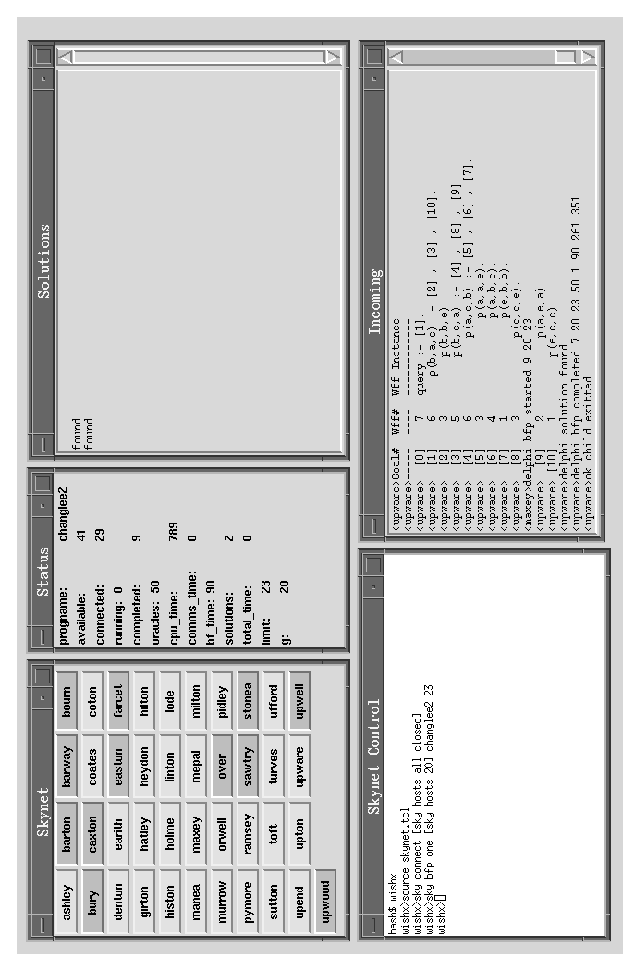
\psfig{file={system/ps/skynet_half_grey.ps}} \hfill}
\caption{Skynet control processor user interface.}
\vspace{5mm}
\label{skynet_half_grey}
\end{figure}

The window labelled ``Skynet Control'' is the command-line interface to skynet,
providing commands such as \texttt{sky\_{}connect} to establish connection with a
\texttt{ppc} daemon, and \texttt{sky\_{}bfp} to initiate the breadth-first
partitioning strategy on all the selected path processors.

The window labelled ``Status'' accumulates runtime information as the
distributed execution of the user program progresses.  In particular, the
\texttt{running} field indicates the number of path processors currently 
executing the user program, and \texttt{completed} shows the number of
path processors which have completed their search and become idle.

The ``Solutions'' window simply displays solutions as they are returned from the
path processors.  The ``Incoming'' window displays the complete log of all communications
from all the path processors.  In the example shown, the solution returned by the
user program is the atom \texttt{found}, to reduce the volume of information
accumulated in the ``Solutions'' window.  The voluminous solution is recorded in
the ``Incoming'' log.

The ``Skynet'' window is a graphical display of the status of each of the
available path processors.  Each button is displayed in one of four colours:
\begin{description}
\item[Grey: ]{Path processor not yet contacted.  A user click on the button will
    cause \texttt{skynet} to connect to the path processor \texttt{ppc} and change
    the button to yellow, or red if the connection fails.}
\item[Yellow: ]{\texttt{skynet} connected to \texttt{ppc}.  A user click will
    disconnect \texttt{skynet} from the path processor \texttt{ppc} and change the
    button back to grey.}
\item[Green: ]{Path processor is currently busy with user process.  A user click
    will send a command to the path processor \texttt{ppc} to
    \textit{kill} the user process.  The button will change back to yellow when
    confirmation of the child exit is received.}
\item[Red: ]{Path processor unavailable.}
\end{description}
When the user issues the \texttt{sky\_{}bfp} command or the \texttt{sky\_{}bfp\_{}one}
command in the ``Skynet Control'' window, the buttons of the selected path
processors will change from yellow to green and the user processes start
execution.  The buttons return to yellow as the path processors complete their
assigned work.

The process \texttt{skyhub} provides a transparent multiplexing function between
\texttt{skynet} and the many \texttt{ppc} daemons.  The primary requirement for
the \texttt{skyhub} process was to overcome the 64 socket-connection limit of
the DECstation 3100's used for the research, although in fact never more than
42 were available.  The \texttt{skyhub} process has facilities for the local
storage and manipulation of variables by the controlling \texttt{skynet}, for
a possible future hierarchical implementation of a partitioning strategy.


\chapter{Benchmarks}
\label{benchmarks}

\section{Queens}

\section{Pentominoes}

\section{Prolog Technology Theorem Prover}

\section{Chang and Lee Example 2}

\section{Overbeek Example 4}

\chapter[Source code for \texttt{kappa}]{Source code for the parallelisation primitive}
\label{kappa_macro}

This appendix gives the source code for the simple parallelisation primitive
supporting oracles and kappa.

To embed the parallelisation support, each user clause is modified to include
a special goal \texttt{o\_{}kbuild(N)} where \texttt{N} is the index of the clause in
the current procedure.  This example program is transformed as
follows:
\begin{verbatim}
a(X) :- b(X), c(X).
a(X) :- d(X).
a(z).

b(X) :- c(X).
b(b).

c(z).
\end{verbatim}
This program becomes:
\begin{verbatim}
a(X) :- o_kbuild(1),b(X), c(X).
a(X) :- o_kbuild(2),d(X).
a(z) :- o_kbuild(3).

b(X) :- o_kbuild(1),c(X).
b(b) :- o_kbuild(2).

c(z) :- o_kbuild(1).
\end{verbatim}

The primitive \texttt{o\_{}kbuild} is implemented as a 'C' macro and treated as
a goal by a stub Prolog procedure:
\begin{verbatim}
o_kbuild(N) :- pragma_c(o_kbuild1).
o_kbuild(_) :- pragma_c(o_kbuild2).
\end{verbatim}

The 'C' macros defining \texttt{o\_{}kbuild1} and \texttt{o\_{}kbuild2} are
as follows:
\begin{verbatim}
#define MAXORC  10000     /* maximum length of oracle            */

static int defer = 0;     /* flag to defer interrupt handling    */
static int skip = 0;      /* flag to skip prev port on interrupt */

static int orc[MAXORC];   /* array to hold orc as it is built    */

static int b_depth;       /* current BUILD or-depth              */

static int orc_l0;        /* depth limit L0                      */
static int orc_l;         /* depth limit L                       */
static int orc_g;         /* group count G                       */
static int orc_n;         /* unique processor number N           */
static int orc_s;         /* count of ports S                    */
static int orc_length;    /* length of oracle to follow          */

#define o_kbuild1      
    { int index;       
      ++b_depth;       
      Deref(A(0),word,tag,adr) 
      index = UnTag_INT(word);  /* index := argument to o_kbuild */
      if (b_depth <= orc_l0) { if (index != orc[b_depth]) fail;}
      else { if (b_depth <= orc_length) 
               { if (index < orc[b_depth]) fail;
                 if (index > orc[b_depth]) orc_length = 0;
               }                               
             orc[b_depth] = index;             
             if (b_depth == orc_l) /* if at partitioning depth...*/
               { if (skip) { skip = 0; fail; } 
                 orc_s++;                      
                 if (orc_s % orc_g != orc_n) fail;
                 if (defer) { defer = 0; send_oracle(); fail; }  
               }                      
           }                          
    }

#define o_kbuild2     /* called on backtracking through o_kbuild */
    {                                 
      b_depth--;                      
      fail;                           
    }
\end{verbatim}

Similar parallelisation primitives which exploit more complex transformations of the
user program are possible (for example see Chapter \ref{bfp_depth}).  Also the
primitive described above could equally be implemented wholly as a 'C' macro without
the use of the stub Prolog procedure.  The most efficient implementation might use
a modified abstract machine. However, the implementation described above
is portable to any Prolog compiler supporting embedded 'C' code, and the simple
definition seems to produce an acceptable overhead of approximately 10\%.

\bibliography{../ijl20}


\end{document}
